\chapter{Исследование суб- и мезомасштабной динамики Океана по оптическим и радиолокационным изображениям} \label{chap:3}



Спутниковые наблюдения Океана в оптическом диапазоне обеспечивают регулярные измерения параметров цвета Океана и поверхностной температуры (ТПО), в полях которых проявляются удивительно красивые пространственные текстуры с масштабами от 1 до 100\textit{км}. Эти текстуры демонстрируют многообразие мезомасштабной динамики верхнего слоя Океана и её взаимосвязь с биологическими процессами.

Наблюдения с помощью радиолокаторов с синтезированной апертурой (РСА), так же очень часто демонстрируют эффектные поверхностные проявления мезо-масштабных и суб-мезомасштабных явлений в Океане, хотя и основаны на других физических принципах. В этом случае поверхностные проявления ассоциируются с контрастами ``шероховатости'' поверхности Океана, вызванные взаимодействием волн с течениями, переменным ветром и влиянием поверхностно-активных веществ (см. например \citep{Marmorino1994, Johannessen1996, Jansen1998, Kudryavtsev2005, Johannessen2005}). Для интерпретации проявлений океанических течений на РСА изображениях был предложен ряд физических моделей (\citep{Alpers1984, Romeiser1997, Kudryavtsev2005}). Не смотря на то, что возможность регистрации океанических явлений радиолокационными методами из Космоса ограничена ``благоприятными'' условиями (малые и умеренные скорости ветра), РСА, благодаря их высокому пространственному разрешению и широкой полосе наблюдения, представляют на данный момент ``мощный'' инструмент для исследования широкого круга океанических явлений, включающих внутренние волны, мезомасштабные особенности течений (включая филаменты), меандрирующие фронты, а так же биологические и нефтяные слики (см. например \citep{Gasparovic1988, Lyzenga1988, Johannessen1996, Beal1997, Espedal1998, Gade1998, Gade1998b}).

В предыдущих главах было показано, что вариации СКН линейно связаны с вариациям яркости морской поверхности через передаточную функцию. Если предположить, что вариации СКН вызваны трансформацией ветровых волн на поверхностных течениях, то динамику Океана можно исследовать по изображениям солнечного блика. В этой главе рассматриваются примеры наблюдения суб- и мезомасштабной изменчивости Океана по данным спутниковых оптических и радиолокационных сенсоров.



\section{Внутренние волны} \label{sec:3.1}


В качестве иллюстрации, разработанный алгоритм применяется к спутниковым оптическим изображениям внутренних волн (ВВ), -- как простейшем типе течений. В качестве примера рассматривается район западно-экваториальной Атлантики, напротив устья реки Амазонки, который является областью регулярного возникновения очень мощных внутренних волн (ВВ), формируемых полусуточными приливными волнами (см. например, \citep{Ivanov1993}). Экспериментальные исследования ВВ и их влияния на обрушения ветровых волн, проведенные в этом районе, представлены в работе \citep{1986}. В этих экспериментах было обнаружено, что интенсивность ВВ коррелировала с фазами Луны, т.е. генерация ВВ имела явно приливное происхождение. В периоды интенсификации ВВ, амплитуды ВВ достигали 100\textit{м}, а при прохождении ВВ (в направлении на Северо-восток, противоположному ветру) на поверхности возникали коррелированные со смещениями термоклина области сильной интенсификации обрушения ветровых волн. Усиление обрушений (в несколько раз по отношению к фоновым значениям) возникало при заглублении термоклина, и почти исчезало при поднятии термоклина, т.е. усиление/подавление обрушений ветровых волн происходило в зонах конвергенции/дивергенции течений индуцированных ВВ на морской поверхности. 

Исходное изображение MODIS/Aqua этого района, полученное 26 апреля 2009, 16:20 показано на Рисунке~\ref{fig:3.1a}.

Несмотря на то, что наблюдаемая область частично покрыта облаками, на снимке легко различимы солнечный блик и вариации яркости внутри блика, связанные с поверхностными проявления ВВ. Также, на Рисунке~\ref{fig:3.1} приводятся поля относительных вариаций яркости $\widetilde{B}/\overline{B}$ (Рисунок~\ref{fig:3.1b}) и передаточная функция $T$ (Рисунок~\ref{fig:3.1c}). Очевидно, что поле относительных вариаций яркости уже содержит признаки ВВ в солнечном блике. Но, в отличие от примера с нефтяным разливом в Мексиканском заливе, в данном случае передаточная функция не имеет зоны инверсии контрастов. Поэтому, как следует из уравнения \eqref{eq:1.7} знак $\widetilde{B}/\overline{B}$ противоположен знаку контрастов СКН.

На Рисунке~\ref{fig:3.1c} приводятся контрасты СКН, отражающие поверхностные проявления ВВ. Поле ВВ имеет характер чередующихся цугов ВВ, распространяющихся в северо-восточном направлении. В начале каждого из цугов идет уединенная волна (солитон).

Расстояние между ведущими солитонами в цугах примерно равно 130-150\textit{км}. Следом за ведущими солитонами распространяются пакеты более коротких ВВ с длинами волн порядка 1\textit{км}. Поскольку предполагается, что источником генерации ВВ в данном районе являются полусуточные приливные волны, по расстоянию между цугами легко оценить фазовую скорость ВВ, которая составляет примерно 3,5\textit{м/c}.



\begin{figure}[H]
   	\centering
	\begin{minipage}{.47\textwidth}
	    \subcaptionbox{\label{fig:3.1a}}
		{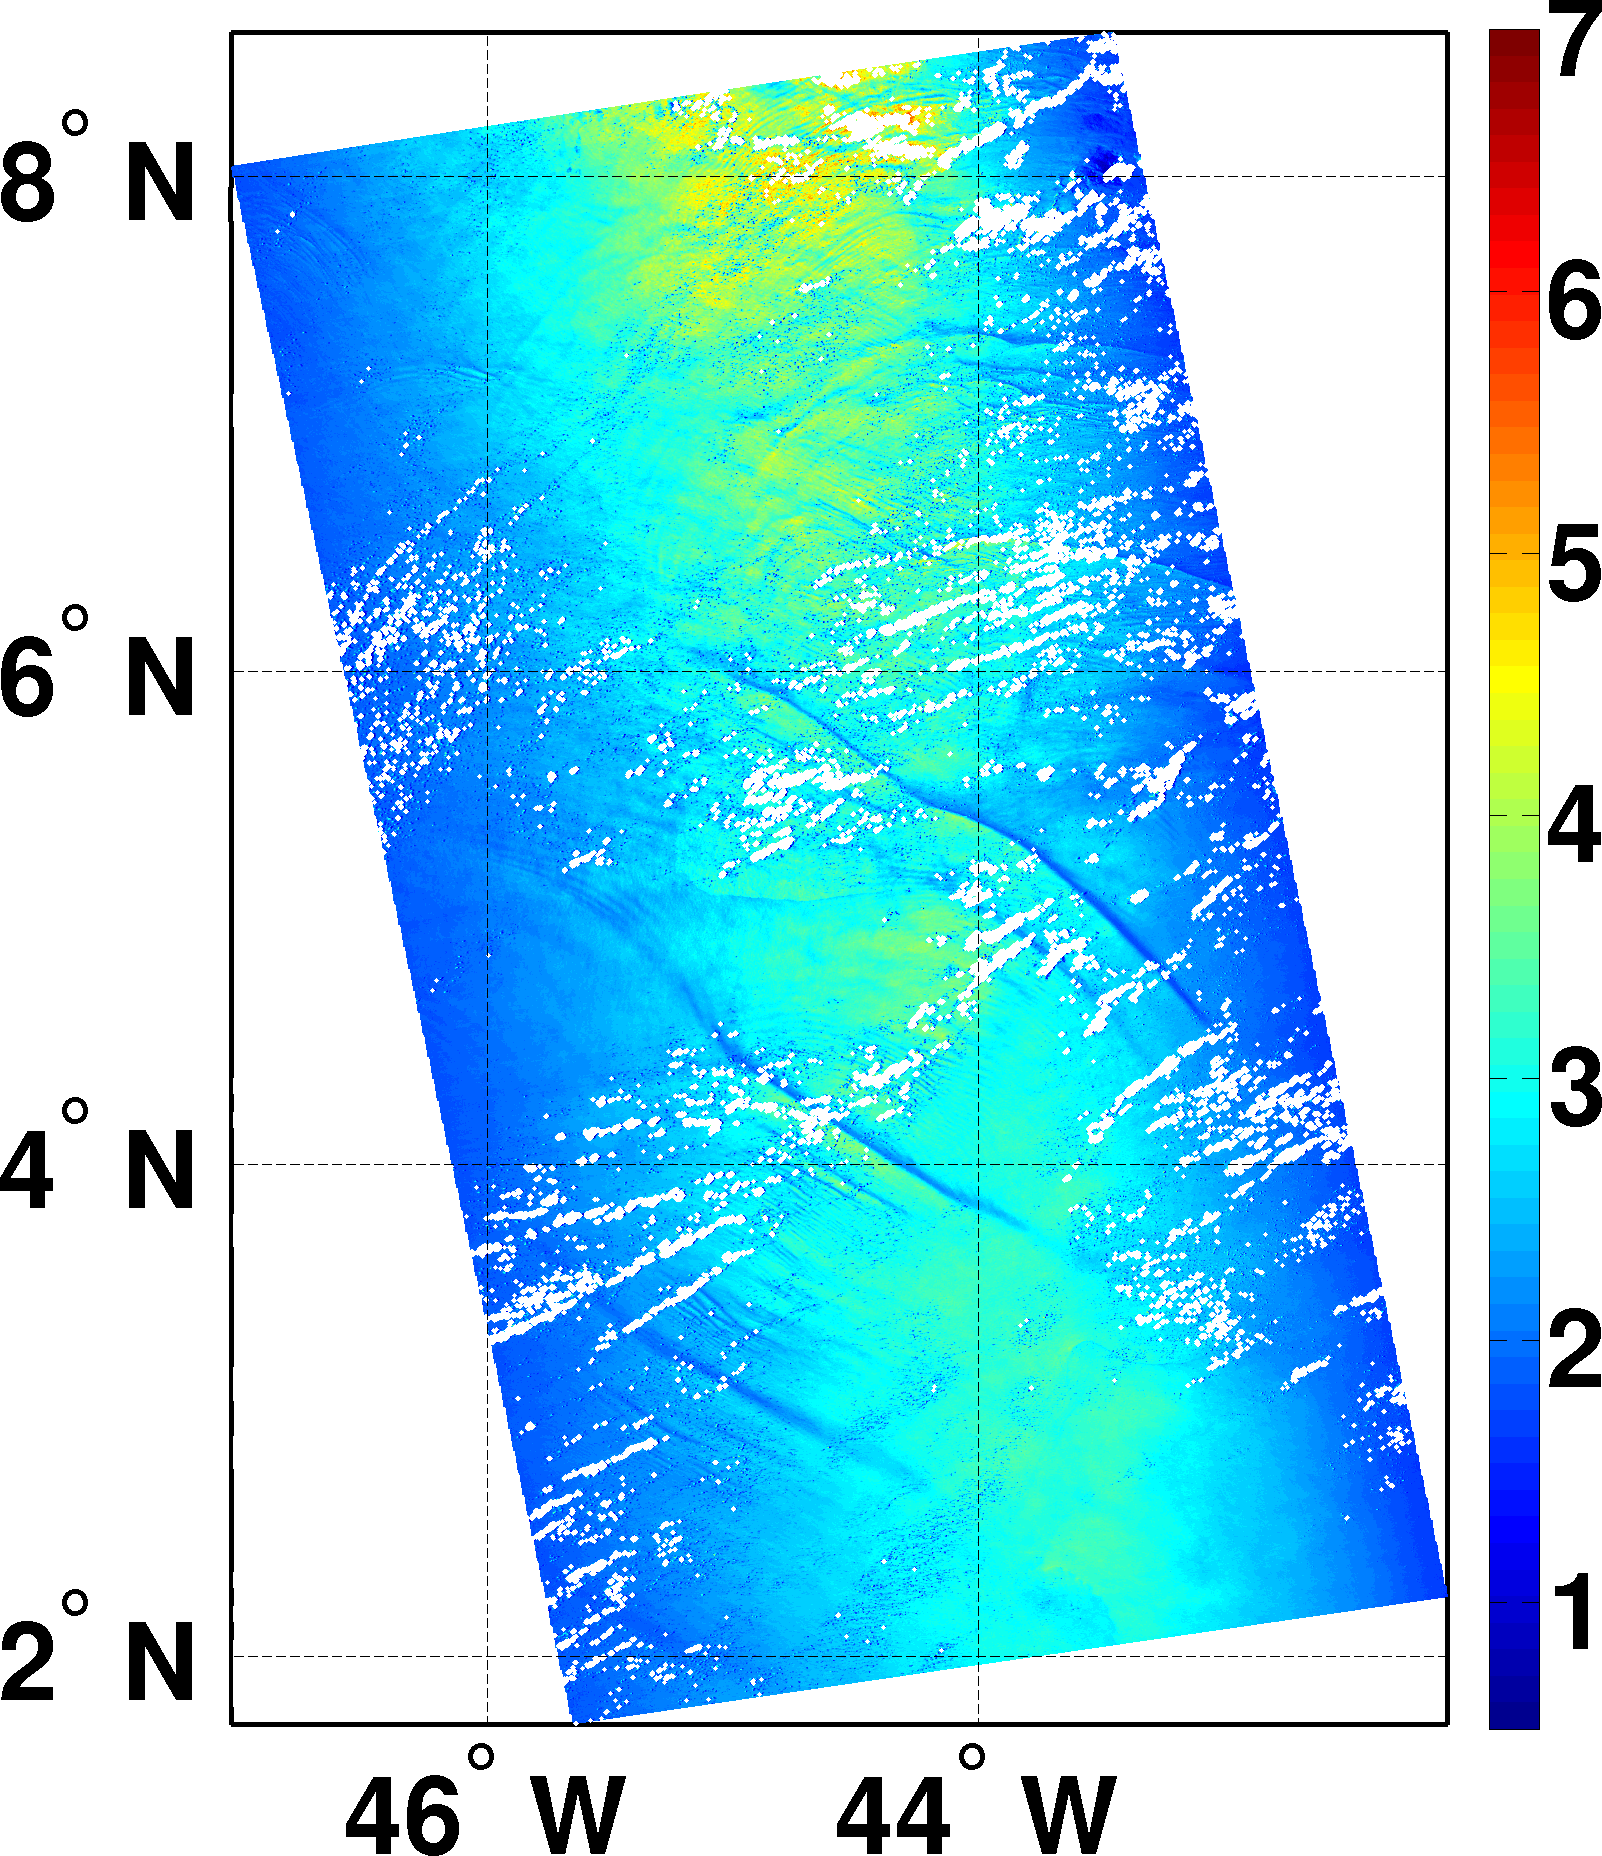
\includegraphics[width=1\linewidth]{fig3_1a}}
	\end{minipage}
	\hfill
	\begin{minipage}{.47\textwidth}
	    \subcaptionbox{\label{fig:3.1b}}
		{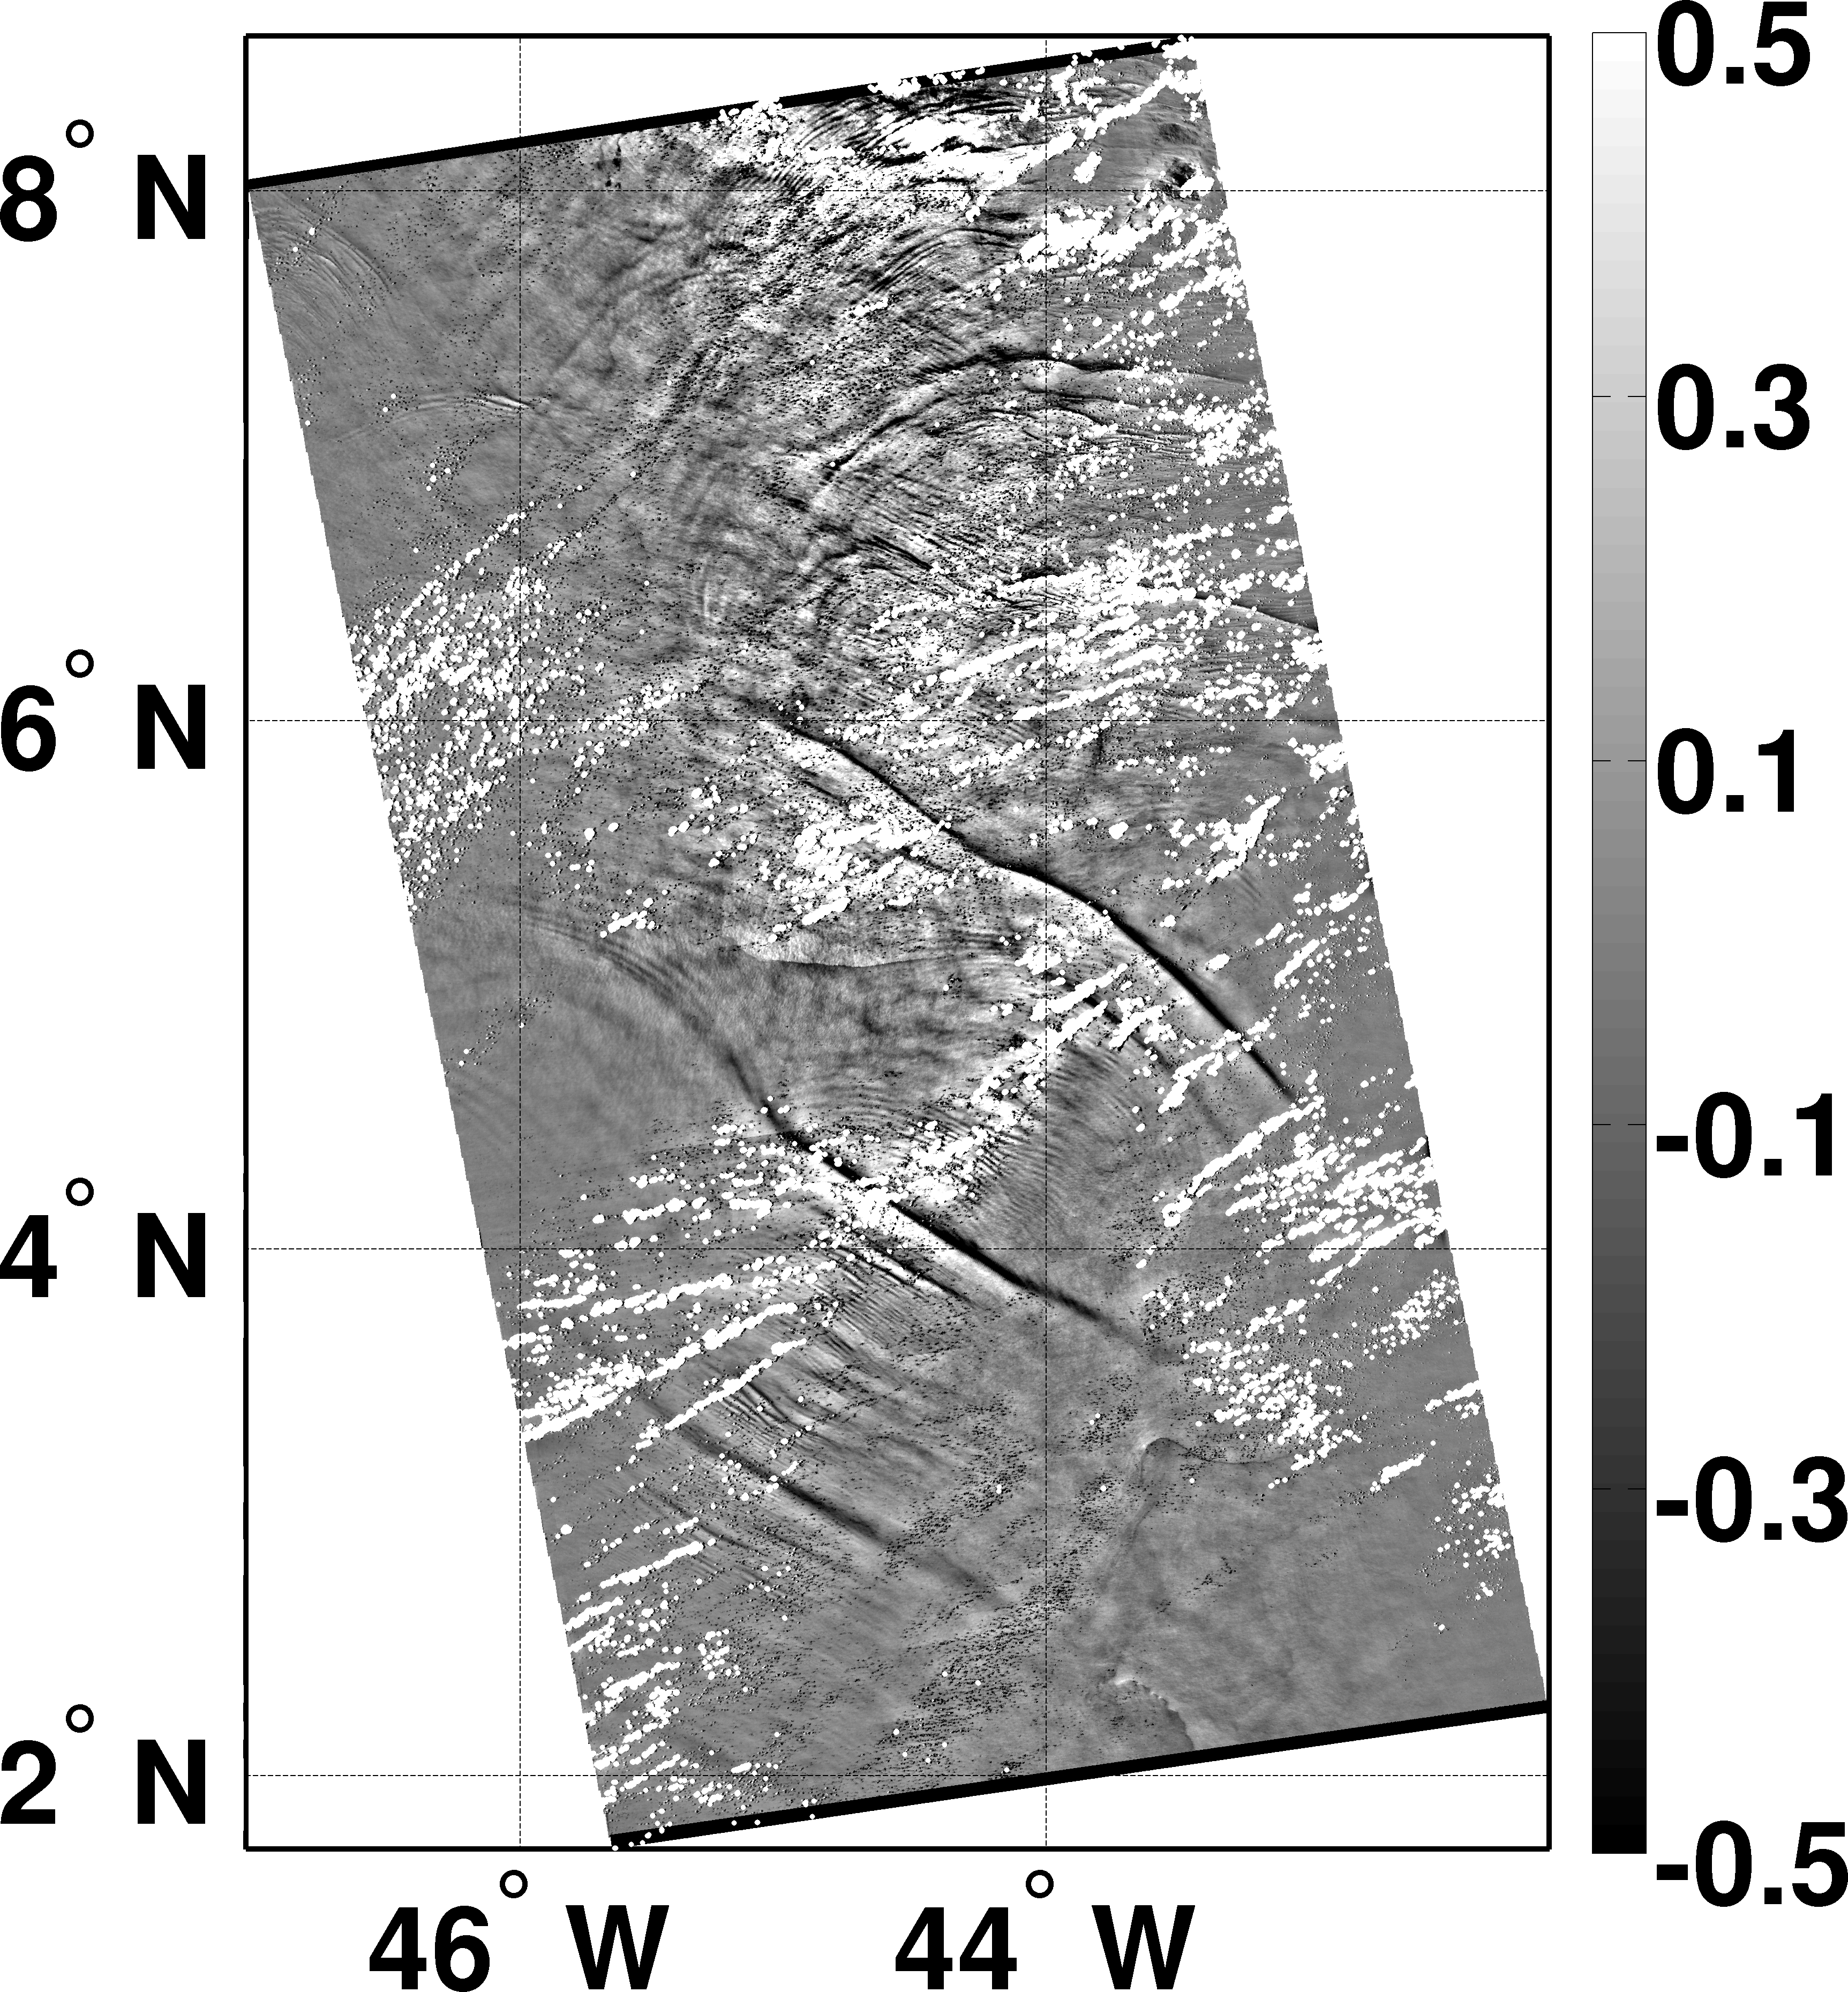
\includegraphics[width=1\linewidth]{fig3_1b}}
	\end{minipage}
	\\
	\begin{minipage}{.47\textwidth}
	    \subcaptionbox{\label{fig:3.1c}}
		{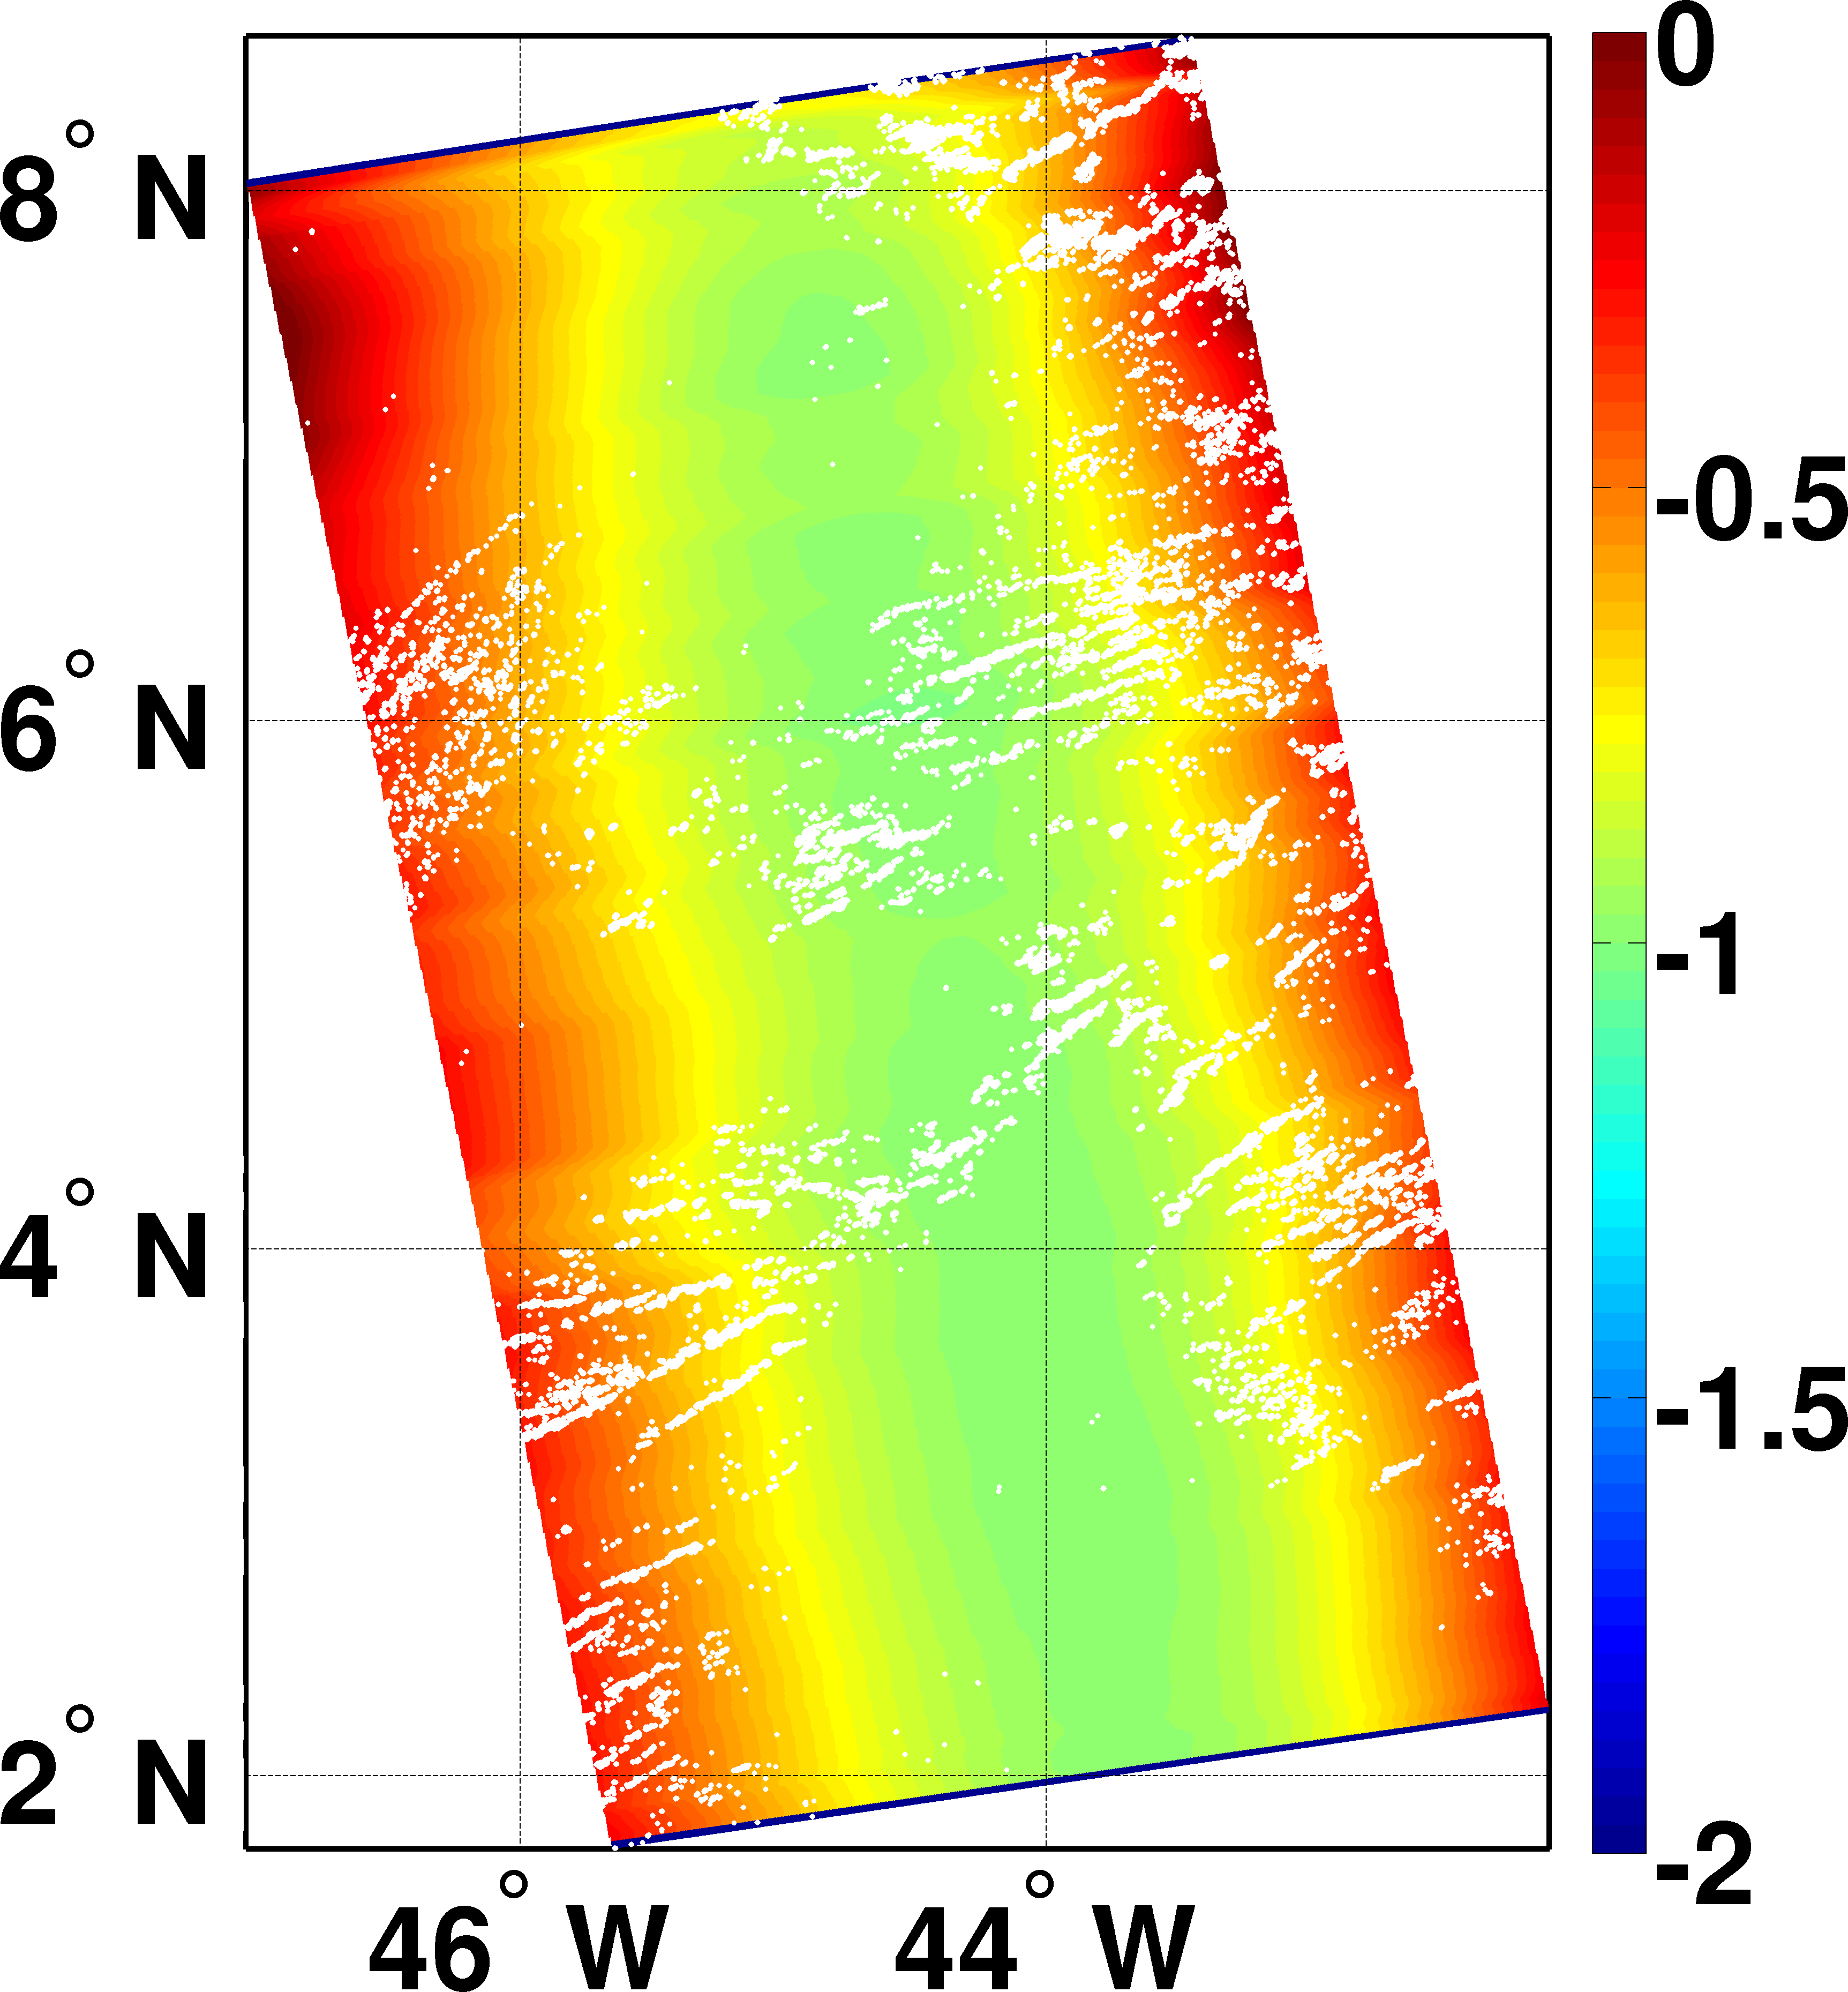
\includegraphics[width=1\linewidth]{fig3_1c}}
	\end{minipage}
	\hfill
	\begin{minipage}{.47\textwidth}
	    \subcaptionbox{\label{fig:3.1d}}
		{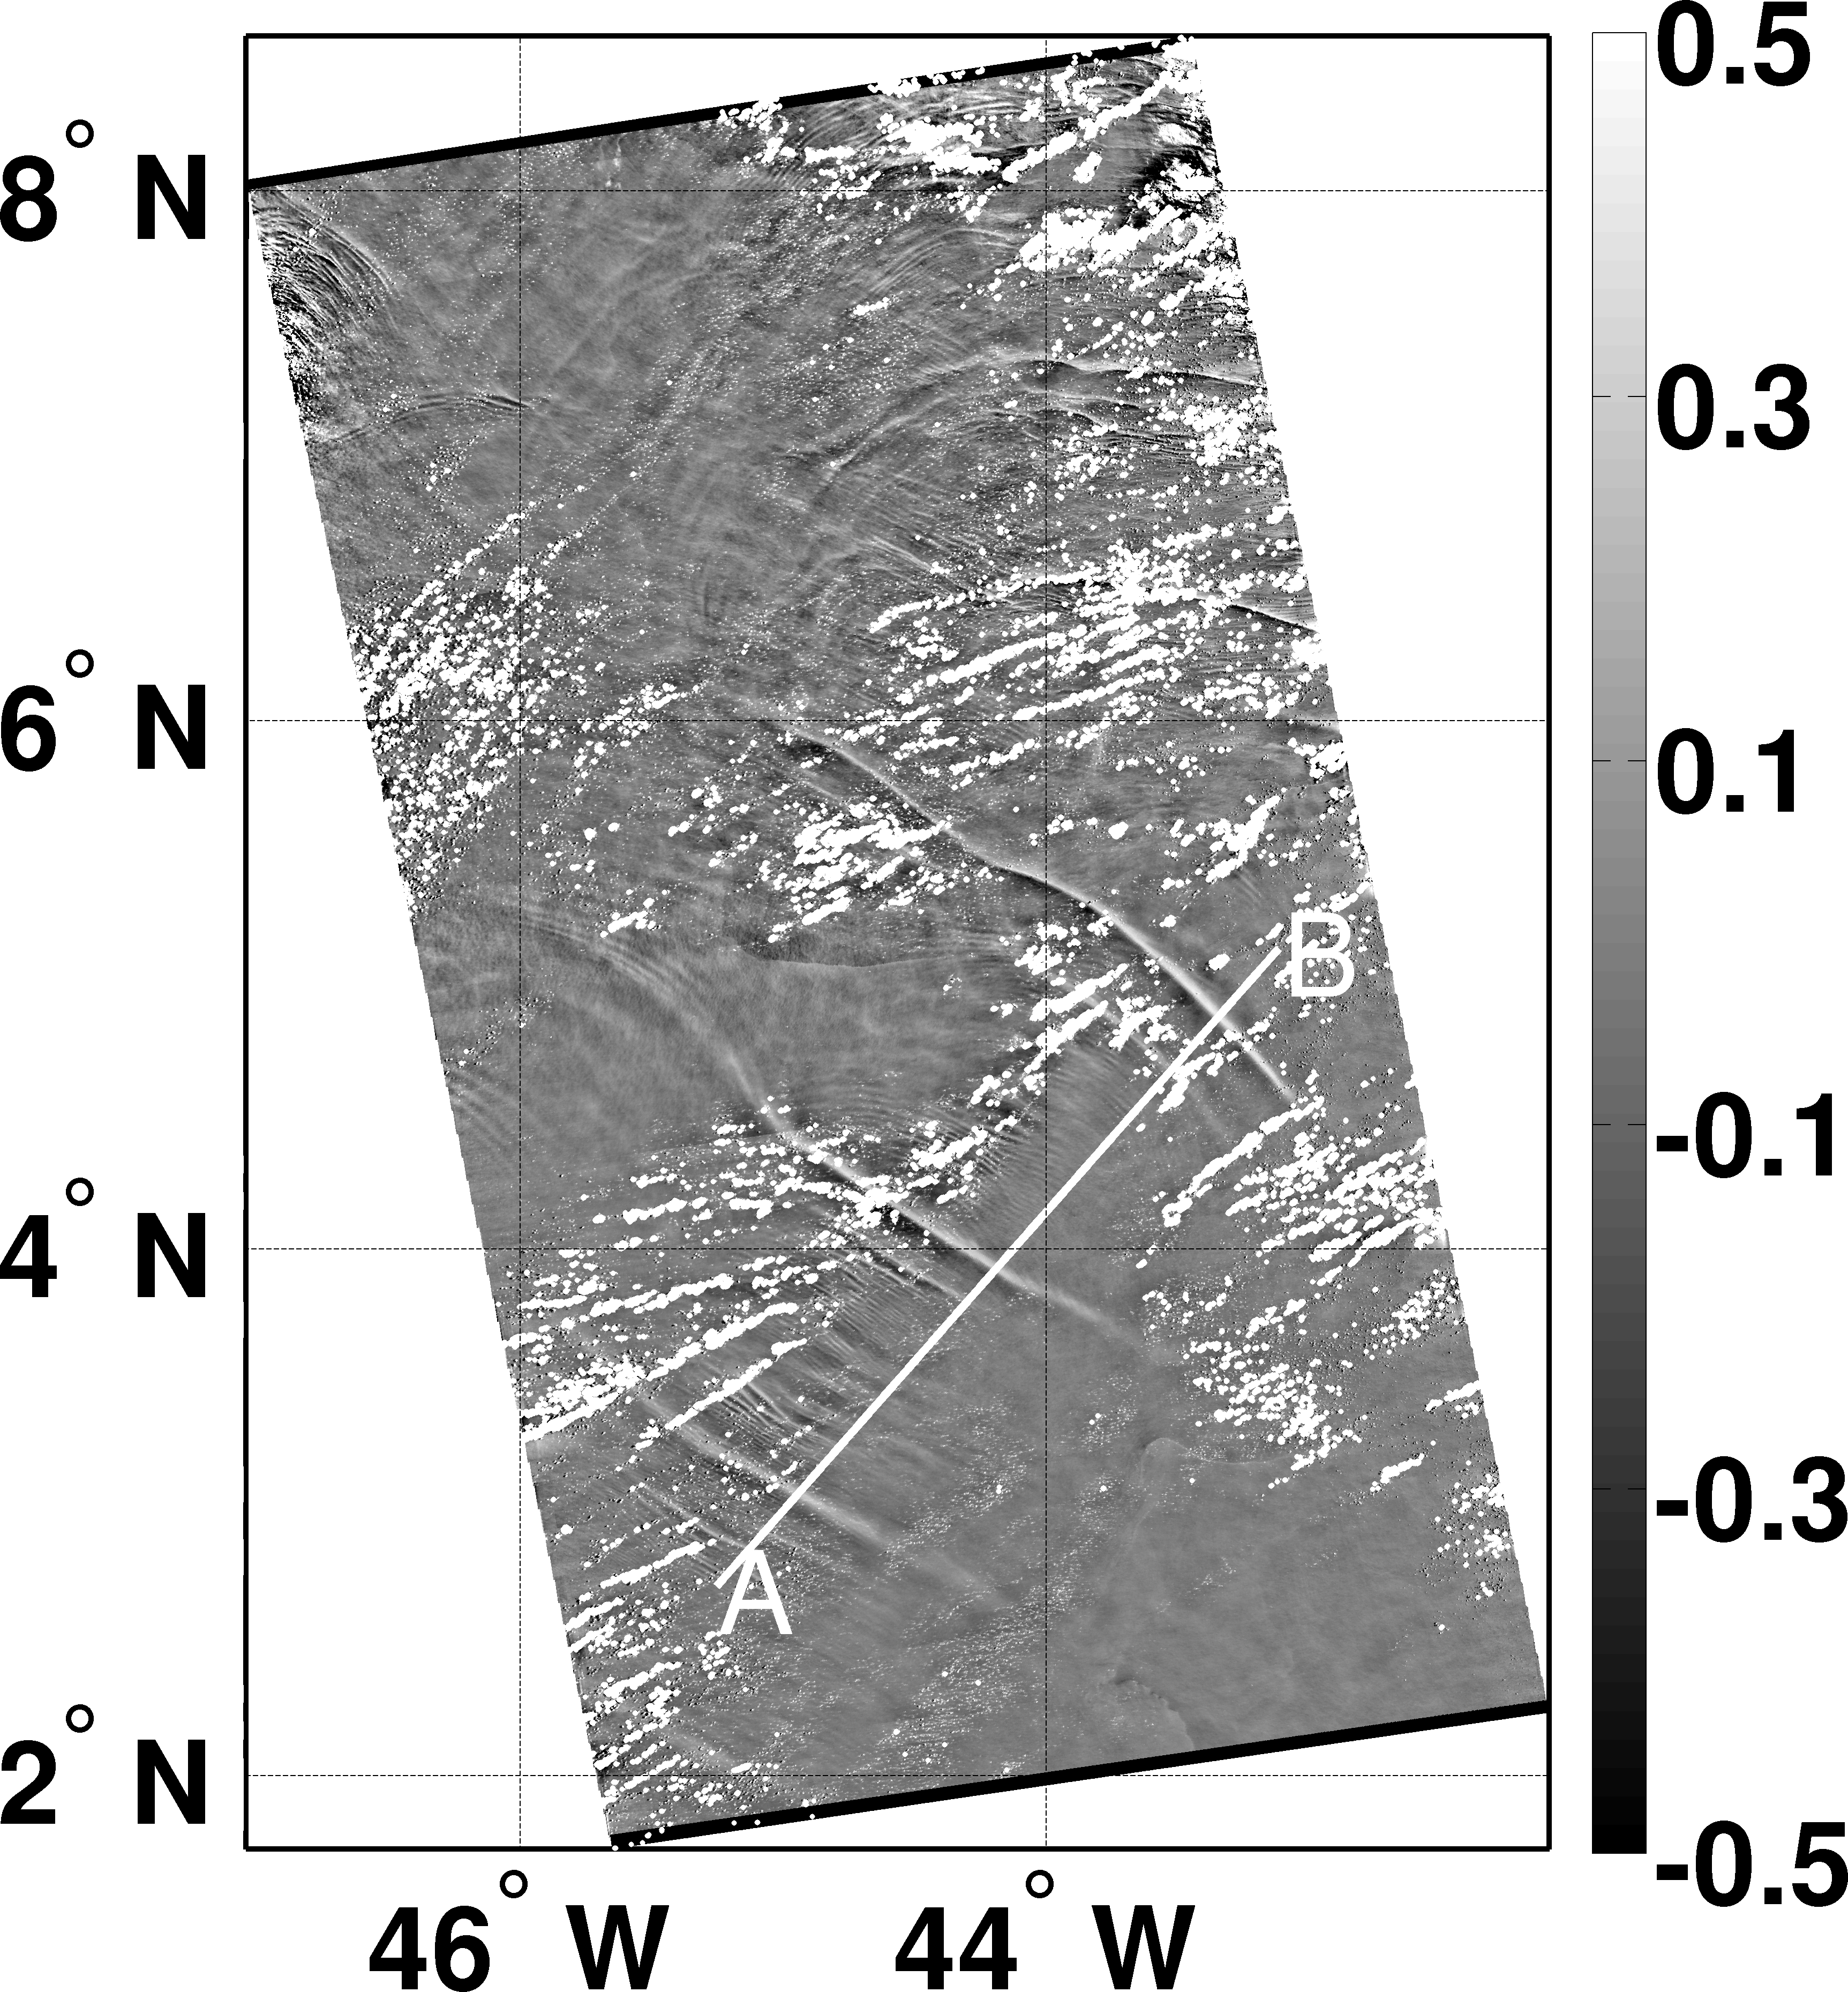
\includegraphics[width=1\linewidth]{fig3_1d}}
	\end{minipage}
    \\
    \floattitle{(а) Фрагмент исходного изображения MODIS/Aqua (26 апреля 2009, 16:20) в красном канале (645~нм) района устья реки Амазонки с признаками ВВ. (б) Контрасты яркости $\widetilde{B}/\overline{B}$. (в) Передаточная функция $T$, заданная уравнениями \eqref{eq:1.7}, \eqref{eq:1.8} и \eqref{eq:1.9}. (г) Контрасты СКН ${\widetilde{s^{2} }\mathord{\left/ {\vphantom {\widetilde{s^{2} } s^{2} }} \right. \kern-\nulldelimiterspace} s^{2} } $. Белые области на изображениях -- маска облаков. Линия A-B обозначает положение сечения, показанного на Рисунке~\ref{fig:3.2}}
    \caption{Фрагмент исходного изображения MODIS/Aqua, обработанный с помощью алгоритма, предложенного в Главе~\ref{chap:1}}
    \label{fig:3.1}
\end{figure}


Профиль вариаций СКН вдоль сечения A-B (отмеченного на Рисунке~\ref{fig:3.1c}) представлен на Рисунке~\ref{fig:3.2},~вверху. Проявление солитонов ВВ в вариациях СКН имеет ``биполярную'' форму, с положительными и отрицательными аномалиями СКН. Исходя из формы солитона ВВ, можно заключить, что повышение/уменьшение СКН имеет место в зонах конвергенции/дивергенции поверхностных течений, вызванных ВВ. Поведение контрастов СКН очень схоже с пространственными вариациями обрушений ветровых волн вызванных ВВ, которые были проанализированы в работе \citep{1986}.



\begin{figure}[H]
    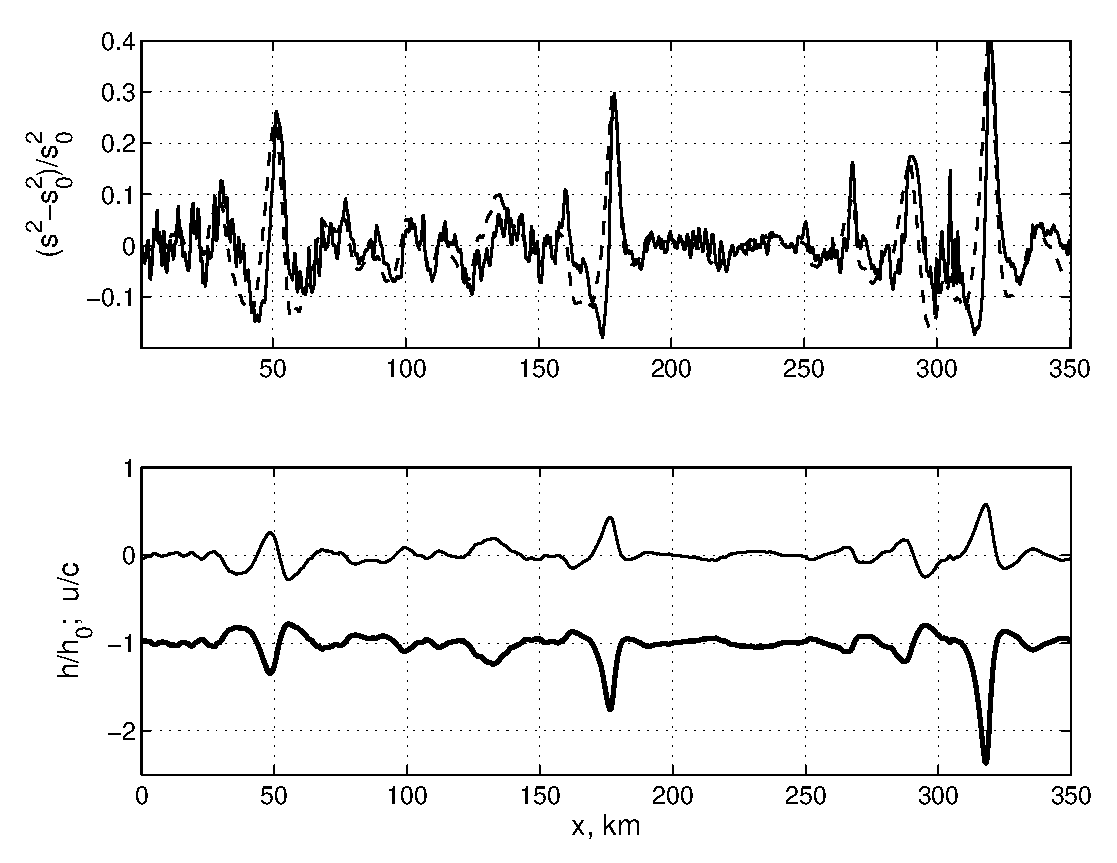
\includegraphics[width=\linewidth]{fig3_2}
    \floattitle{(вверху) Профиль контрастов СКН (сплошная линия) вдоль сечения A-B, показанного на Рисунке~\ref{fig:3.1c}. Пунктирная линия отражает RIM моделирование. (внизу) Смещение термоклина ВВ-ой (жирная линия) и скорость течения на поверхности, вызванное ВВ (тонкая линия)}
    \caption{Профиль контрастов СКН и RIM моделирование сечения, проходящего через ВВ на Рисунке~\ref{fig:3.1c}}
    \label{fig:3.2}
\end{figure}


Для анализа наблюдаемых вариаций СКН нами были проведены модельные расчёты с использованием модели формирования радиолокационных изображений (RIM), предложенной в работе \citep{Kudryavtsev2005}. (см. Приложение~\ref{AppendixA} с описанием модели) В качестве первого предположения можно положить, что наблюдаемое увеличение/уменьшение СКН морской поверхности однозначно связано с конвергенцией/дивергенцией поверхностных течений, вызванных ВВ, т.е. $K_{s} \equiv \tilde{s}^{2} /s_{0}^{2} \propto \partial u/\partial x$. Коэффициент пропорциональности в этом уравнении есть функция скорости ветра и параметров ВВ. Для заданных условий, его можно задать подгоночной константой $c_{u} $, которая определяется сравнением наблюдаемым и модельным СКН. Тогда, поверхностная скорость определяется как



\begin{equation} \label{eq:3.1} u(x)=c_{u} \int _{0}^{x}\left(K_{s} -\left\langle K_{s} \right\rangle \right)dx ,  \end{equation} 



\noindent где $\left\langle K_{s} \right\rangle $ - ``низкочастотные'' колебания СКН (вызванные, например, вариациями скорости ветра), которые не видны на представленных данных, но, приводящие к ``искусственному'' вкладу в $u(x)$, благодаря кумулятивному интегрированию. Эти ``низкочастотные'' осцилляции были вычтены из исходных данных СКН.

Далее, поверхностная скорость течений, определенная соотношением \eqref{eq:3.1}, задавалась в качестве входного параметра для модельных расчетов поверхностных проявлений ВВ по модели RIM. В этих расчетах средняя скорость ветра принята равной 7\textit{м/с}, направление ветра -- противоположным направлению распространения ВВ, а фазовая скорость ВВ задана как c=3.5\textit{м/с}. Значение постоянной $c_{u} $ выбиралась таким образом, чтобы значения вариаций СКН в пиках (над солитонами ВВ) соответствовало бы наблюдаемым значениям. Модельные контрасты СКН показаны на Рисунке~\ref{fig:3.2},~верхний график. Как следует из этого рисунка (Рисунок~\ref{fig:3.2}), профиль модельных контрастов согласуется с наблюдаемым полем вариаций СКН. Это факт позволяет заключить, что наблюдаемые модуляции СКН, в действительности, определяются конвергенцией и дивергенцией течений, индуцируемой ВВ на поверхности. образованных ВВ.

Поле поверхностной скорости $u(x)$, индуцируемое ВВ, а так же как соответствующая глубина залегания термоклина $h(x)$ (рассчитанная с использованием формулы $u/c=(h-h_{0} )/h$, где $h_{0} $ - невозмущённая глубина) приведены на Рисунке~\ref{fig:3.2},~нижний график. Полагая h0=100\textit{м}, амплитуды смещения термоклина $h-h_{0} $ для двух ведущих солитонов составляют 120\textit{м} и 80\textit{м}, что согласуется с данными измерений (Dulov et al., 1986) в этом районе.



\section{Мезомасштабные течения} \label{sec:3.2}



\subsection{Наблюдения} \label{sec:3.2.1}


Данное исследование основано на синергетическом анализе изображений MODIS и ASAR района течения мыса Игольный (Рисунок~\ref{fig:3.3}). Этот район характеризуется интенсивным переносом водных масс, который обеспечивает многообразие мезомасштабной динамики (вихри, грибовидные структуры, температурные фронты, внутренние волны, зыбь и многие другие явления проявления океанической динамики).

Данные ASAR и MODIS/Aqua в районе исследования были получены 18 ноября 2007~г., в 7 ч.~24 мин. и 12 ч.~05 мин., соответственно. На Рисунке~\ref{fig:3.3} приводятся два основных продукта ASAR и MODIS -- поле ветра, полученное по изображению ASAR WS, с использованием алгоритма CMOD4, и поле температуры поверхности Океана (ТПО), полученное по данным MODIS \citep{Brown1999}.

Поле ТПО раскрывает разнообразие мезо- и крупномасштабных особенностей на поверхности основного течения мыса Игольный. Аналогичные особенности можно наблюдать и в поле концентрации хлорофилла, полученного по данным MODIS (здесь не приводится). Поле приводного ветра в данном районе сильно изменчиво, скорость ветра варьируется от 4\textit{м/с} до 13\textit{м/с}, что очевидно отображается на РСА изображении. С другой стороны на данных поля ветра ASAR легко различимы квазилинейные структуры (между 34 и 36 градусом южной широты и 26 и 30 градусом восточной долготы), которые можно трактовать как особенности проявления океанического течения. Далее приводится более детальный анализ описанных особенностей.

На исходном изображении MODIS/Aqua района мыса Игольный в красном канале (850\textit{нм}) разрешением 250\textit{м}, приведённом на Рисунке~\ref{fig:3.4a}, легко различимы облака и солнечный блик. К особенностям этого изображения стоит отнести полосчатую структуру изображения в области солнечного блика, присущую изображениям MODIS. Особенностях формирования изображений MODIS, приводящие к подобной структуре изображения, обсуждались в разделе~\ref{sec:1.4}, а также в статьях~\citep{Myasoedov2010a, Myasoedov2010}. Стоит так же обратить внимание на правый край солнечного блика, где различима особенность, напоминающая океанический вихрь.



\begin{figure}[H]
   	\centering
	\begin{minipage}{.47\textwidth}
	    \subcaptionbox{\label{fig:3.3a}}
		{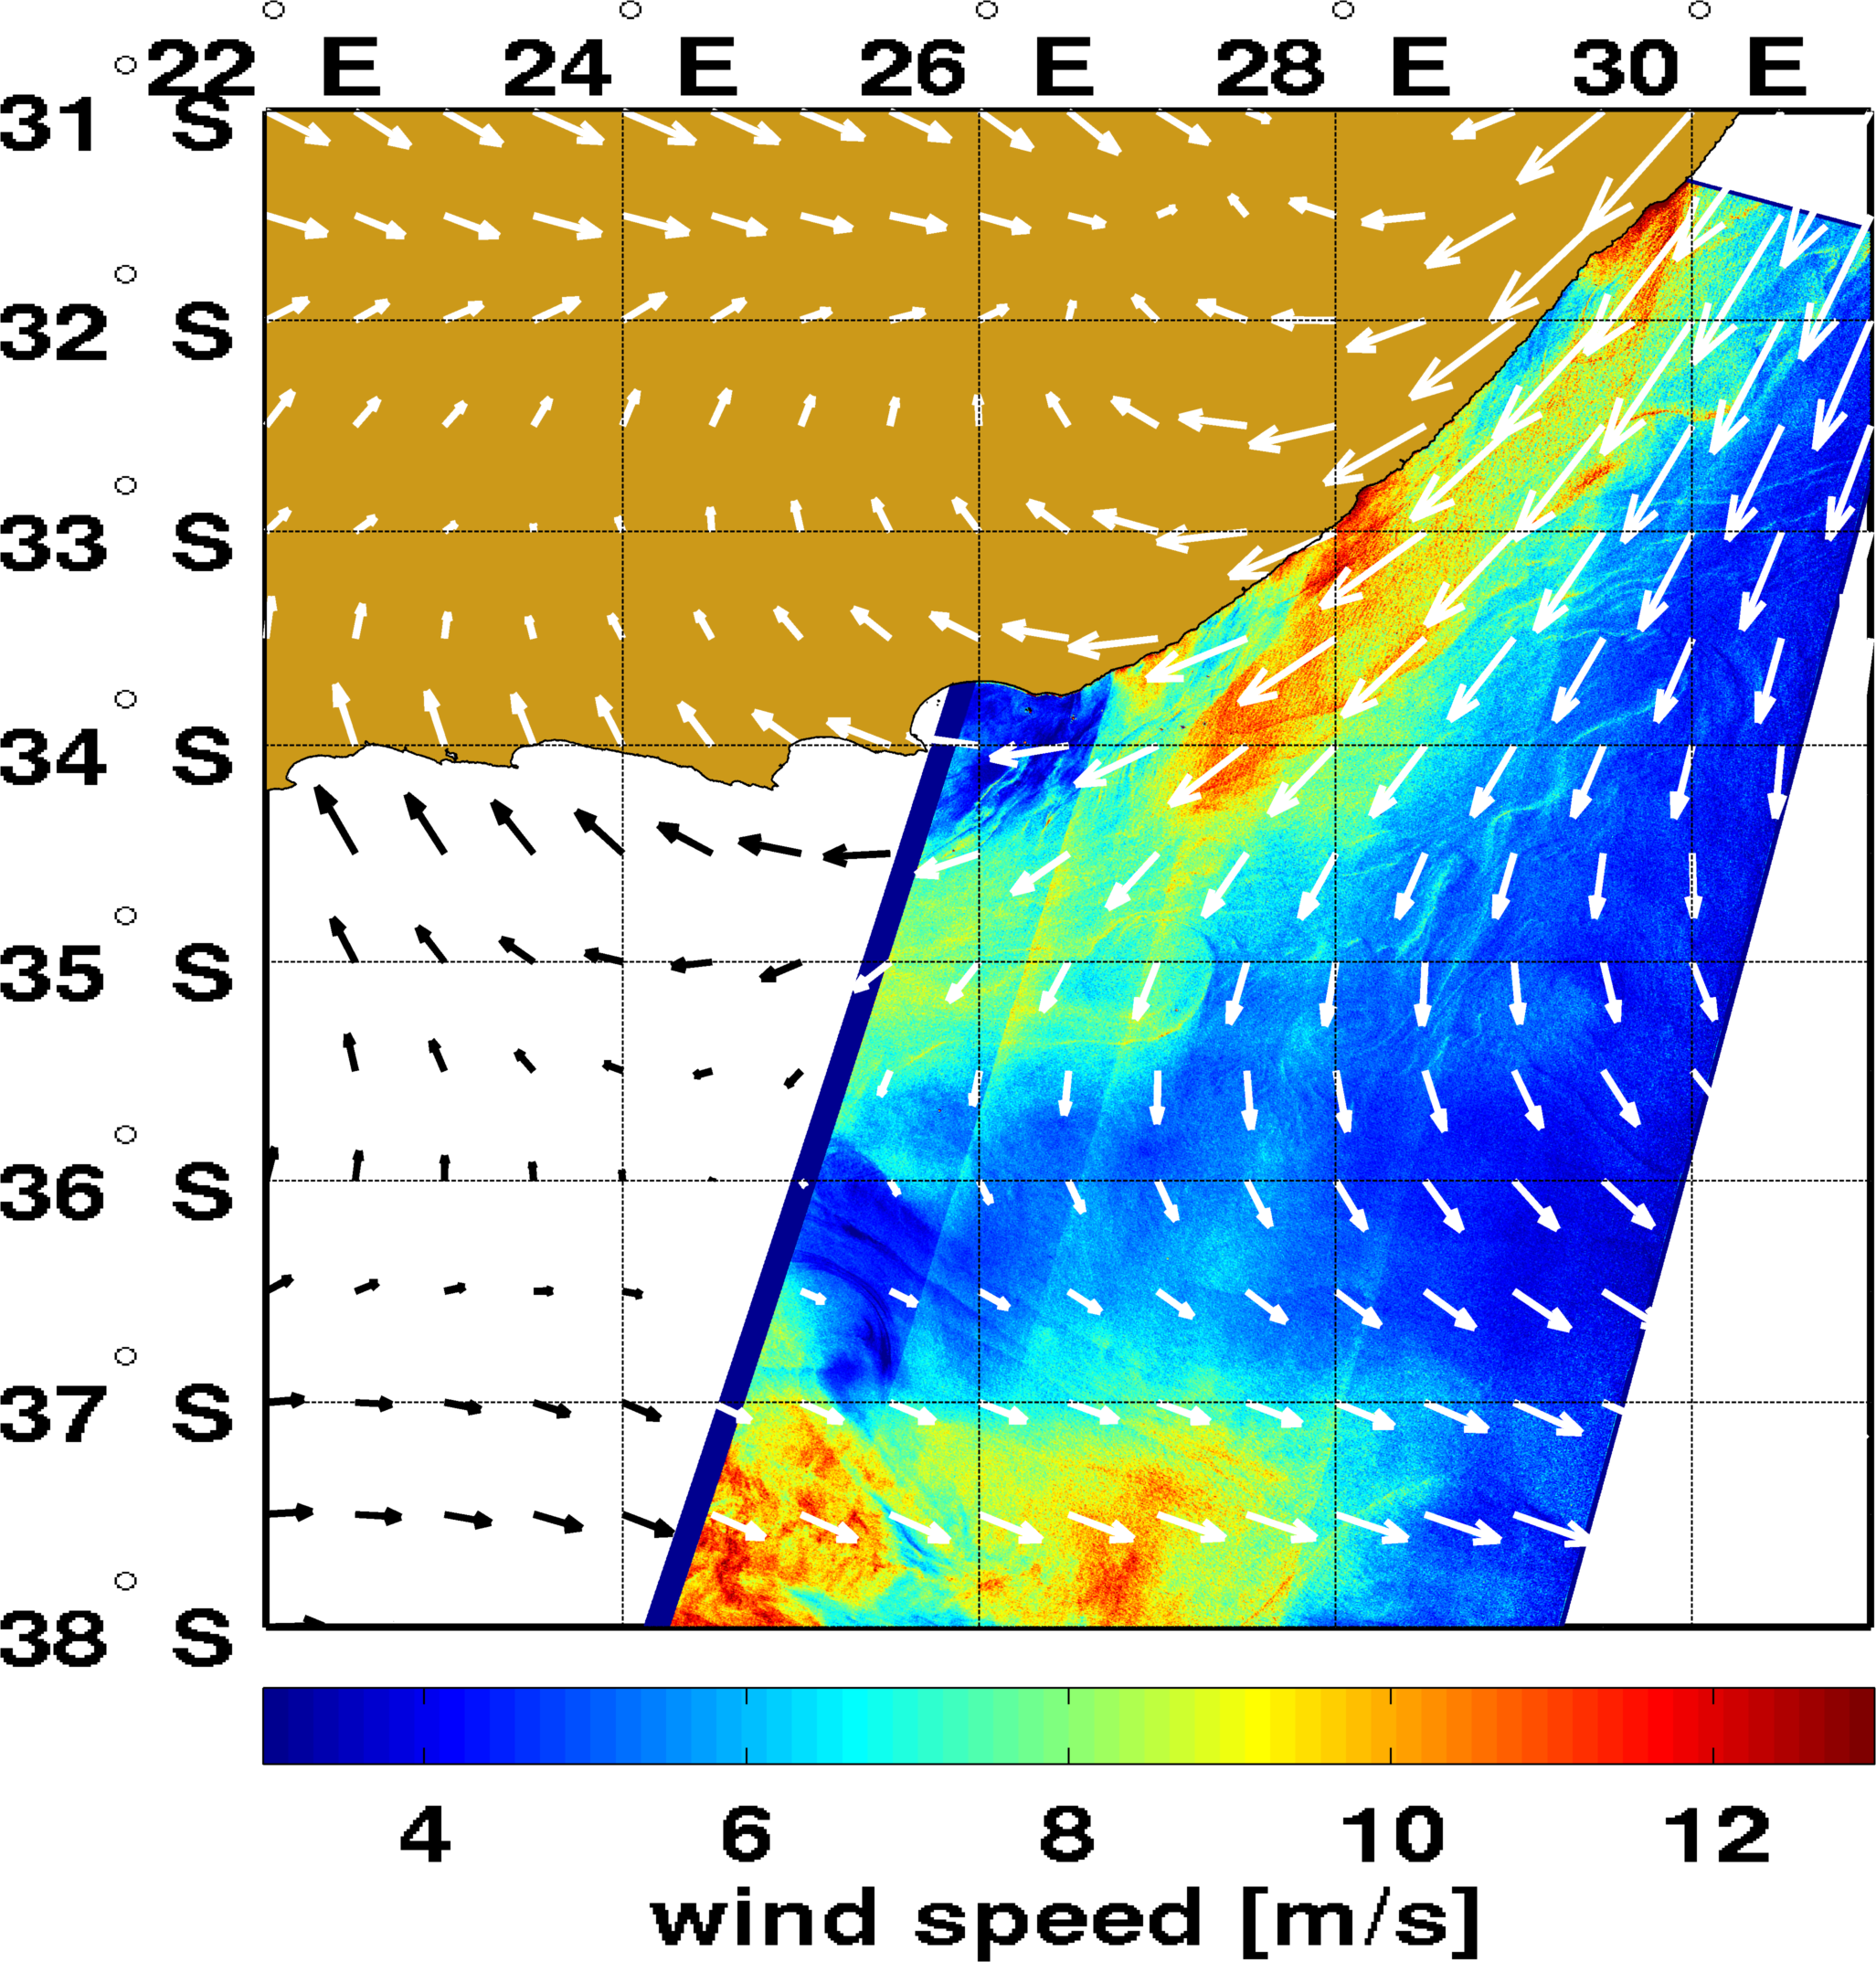
\includegraphics[width=1\linewidth]{fig3_3a}}
	\end{minipage}
	\hfill
	\begin{minipage}{.47\textwidth}
	    \subcaptionbox{\label{fig:3.3b}}
		{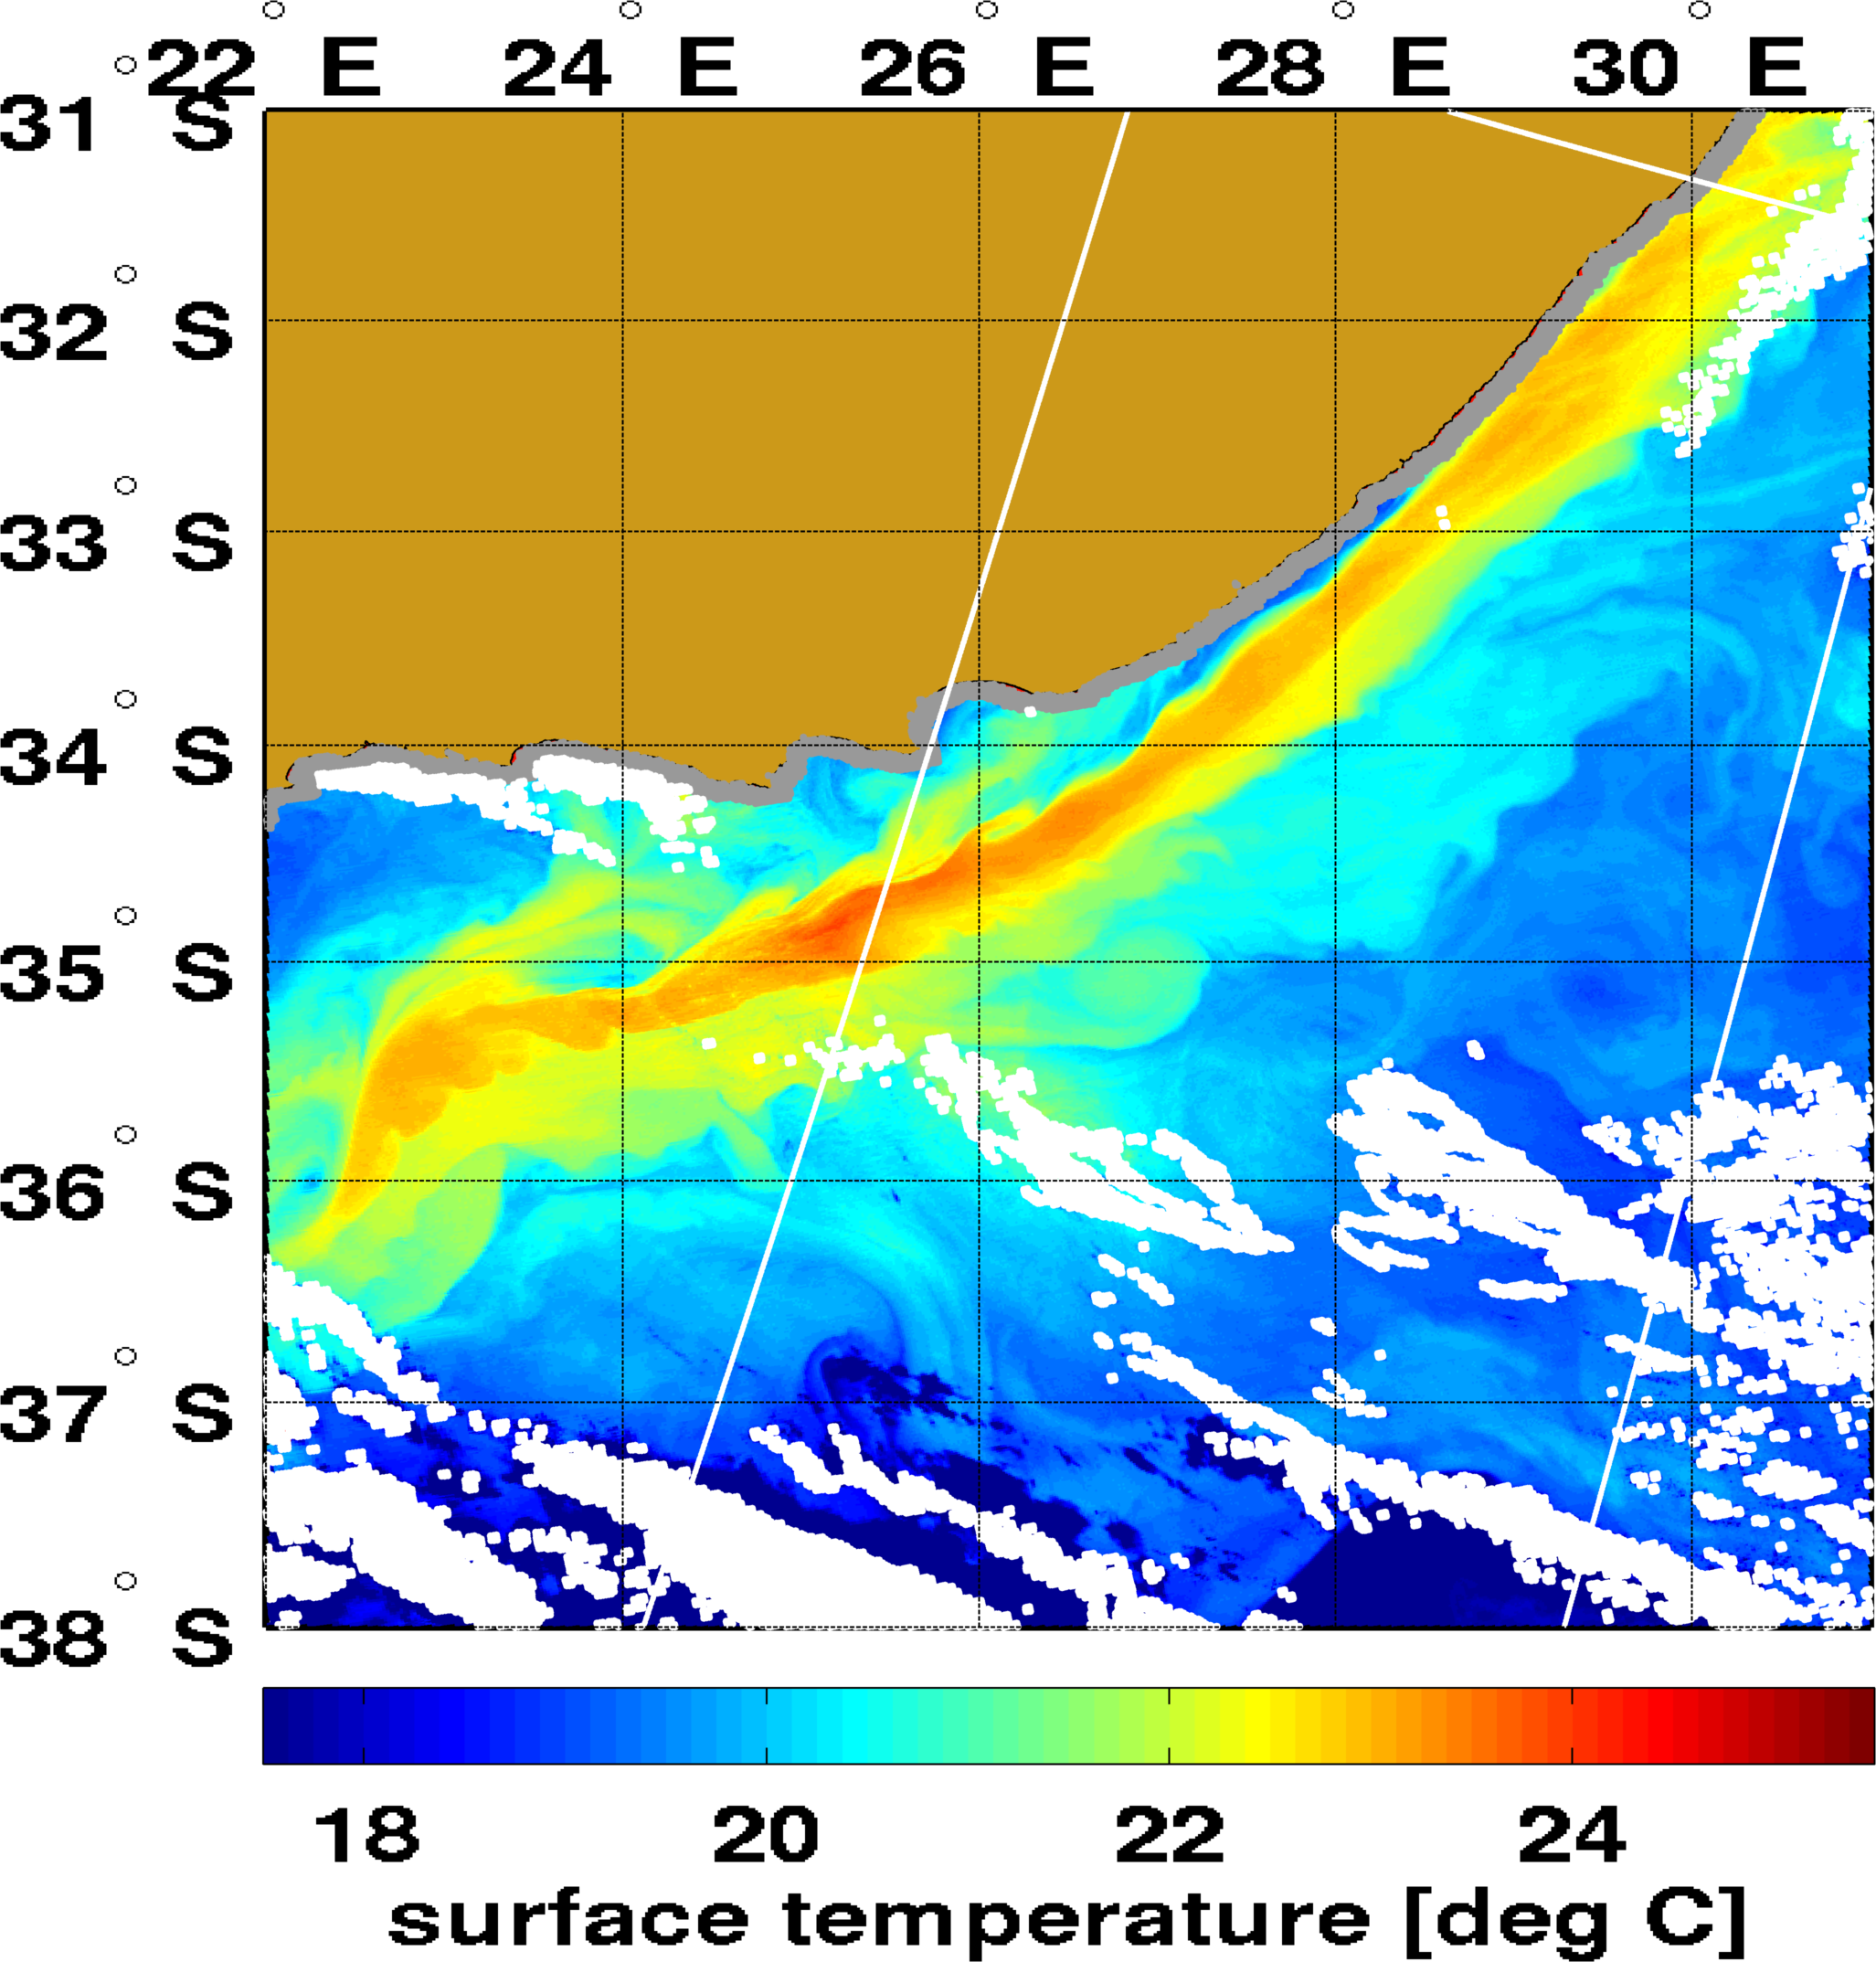
\includegraphics[width=1\linewidth]{fig3_3b}}
	\end{minipage}
    \\
    \floattitle{(а) Поле ветра, восстановленное по данным ASAR WS, с использованием алгоритма CMOD4. Направление ветра взято из модели NCEP. (б) поле поверхностной температуры Океана, полученное по данным MODIS. Белые области - маска облаков. Юг Африканского континента выделен коричневым цветом}
    \caption{Поле ветра и поле поверхностной температуры Океана}
    \label{fig:3.3}
\end{figure}


Используя алгоритм представленный в Главе~\ref{chap:1}и опубликованный в \citep{Kudryavtsev2010,Myasoedov2010a,Myasoedov2010}, исходное изображение раскладывается на составляющие: усреднённые яркости $\bar{B}$ (масштаб осреднения 30x30\textit{км${}^2$}) и их вариации $\tilde{B}$. Последние приведены на Рисунке~\ref{fig:3.4b}. Здесь и далее мы опускаем детали восстановления СКН, отметим, что данные MODIS и MERIS обрабатывались в соответствии с методом, описанным в разделе~\ref{sec:1.3} Главы~\ref{chap:1}.



\begin{figure}[H]
   	\centering
	\begin{minipage}{.47\textwidth}
	    \subcaptionbox{\label{fig:3.4a}}
		{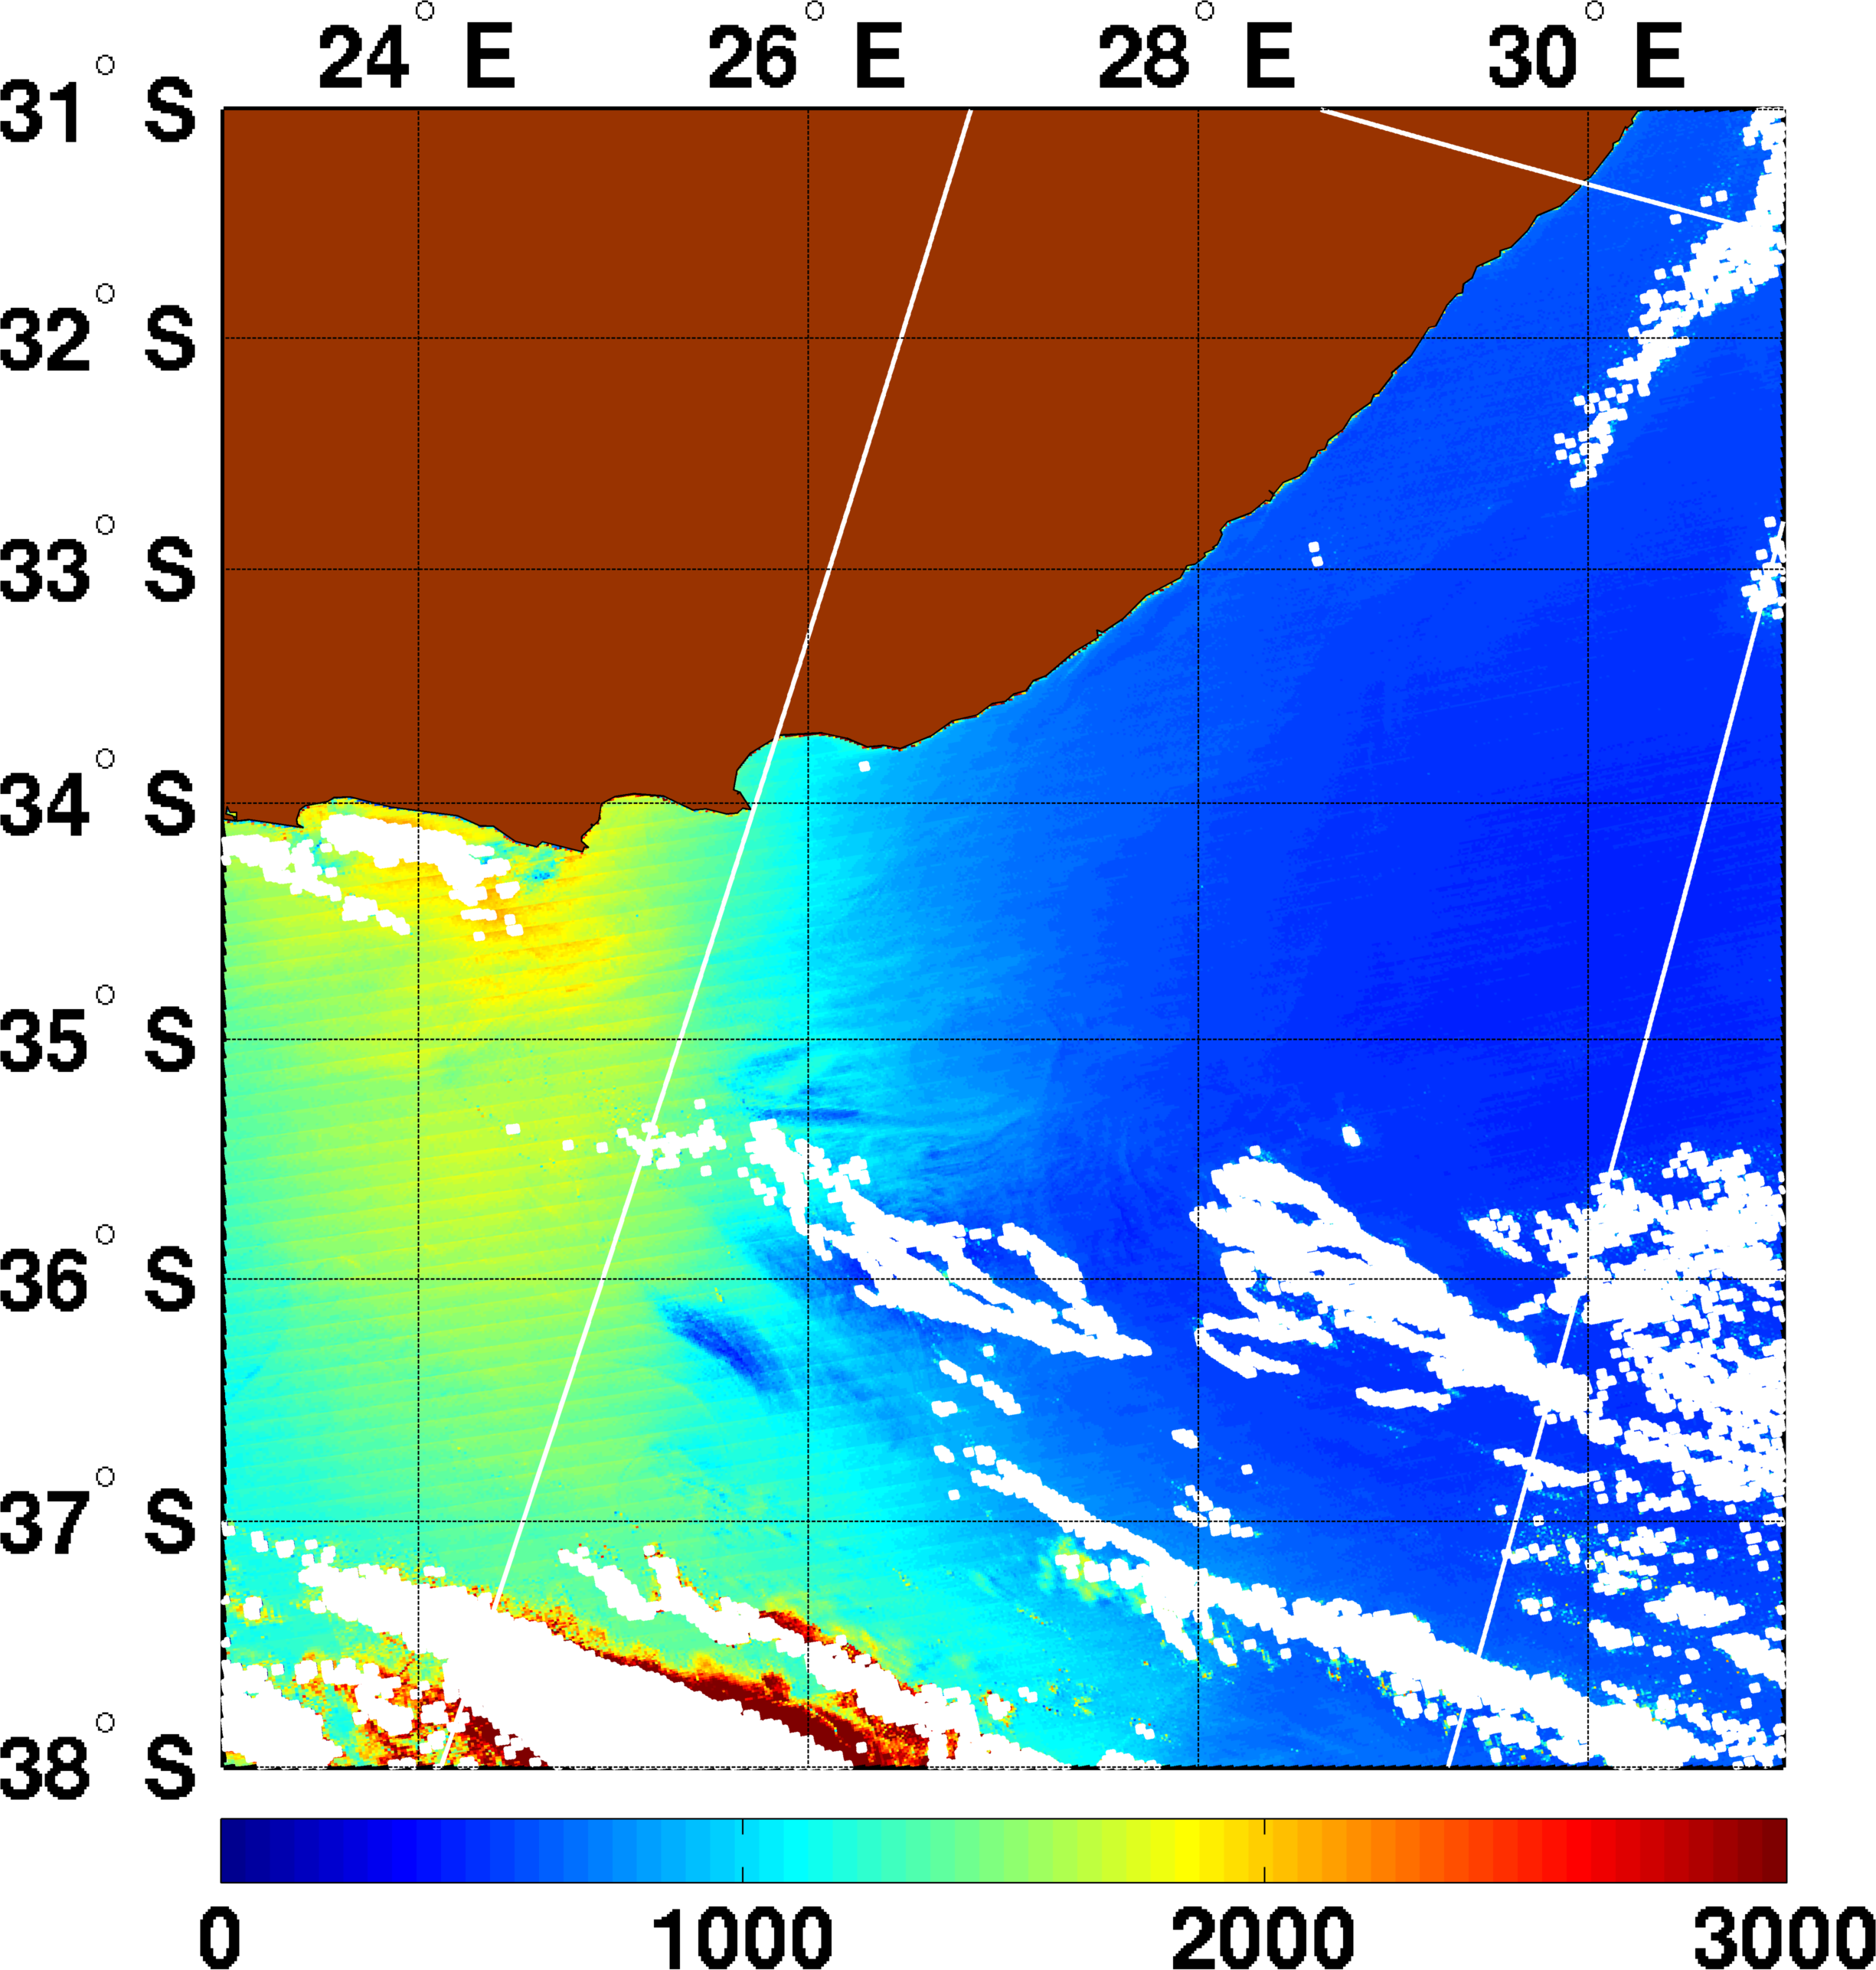
\includegraphics[width=1\linewidth]{fig3_4a}}
	\end{minipage}
	\hfill
	\begin{minipage}{.47\textwidth}
	    \subcaptionbox{\label{fig:3.4b}}
		{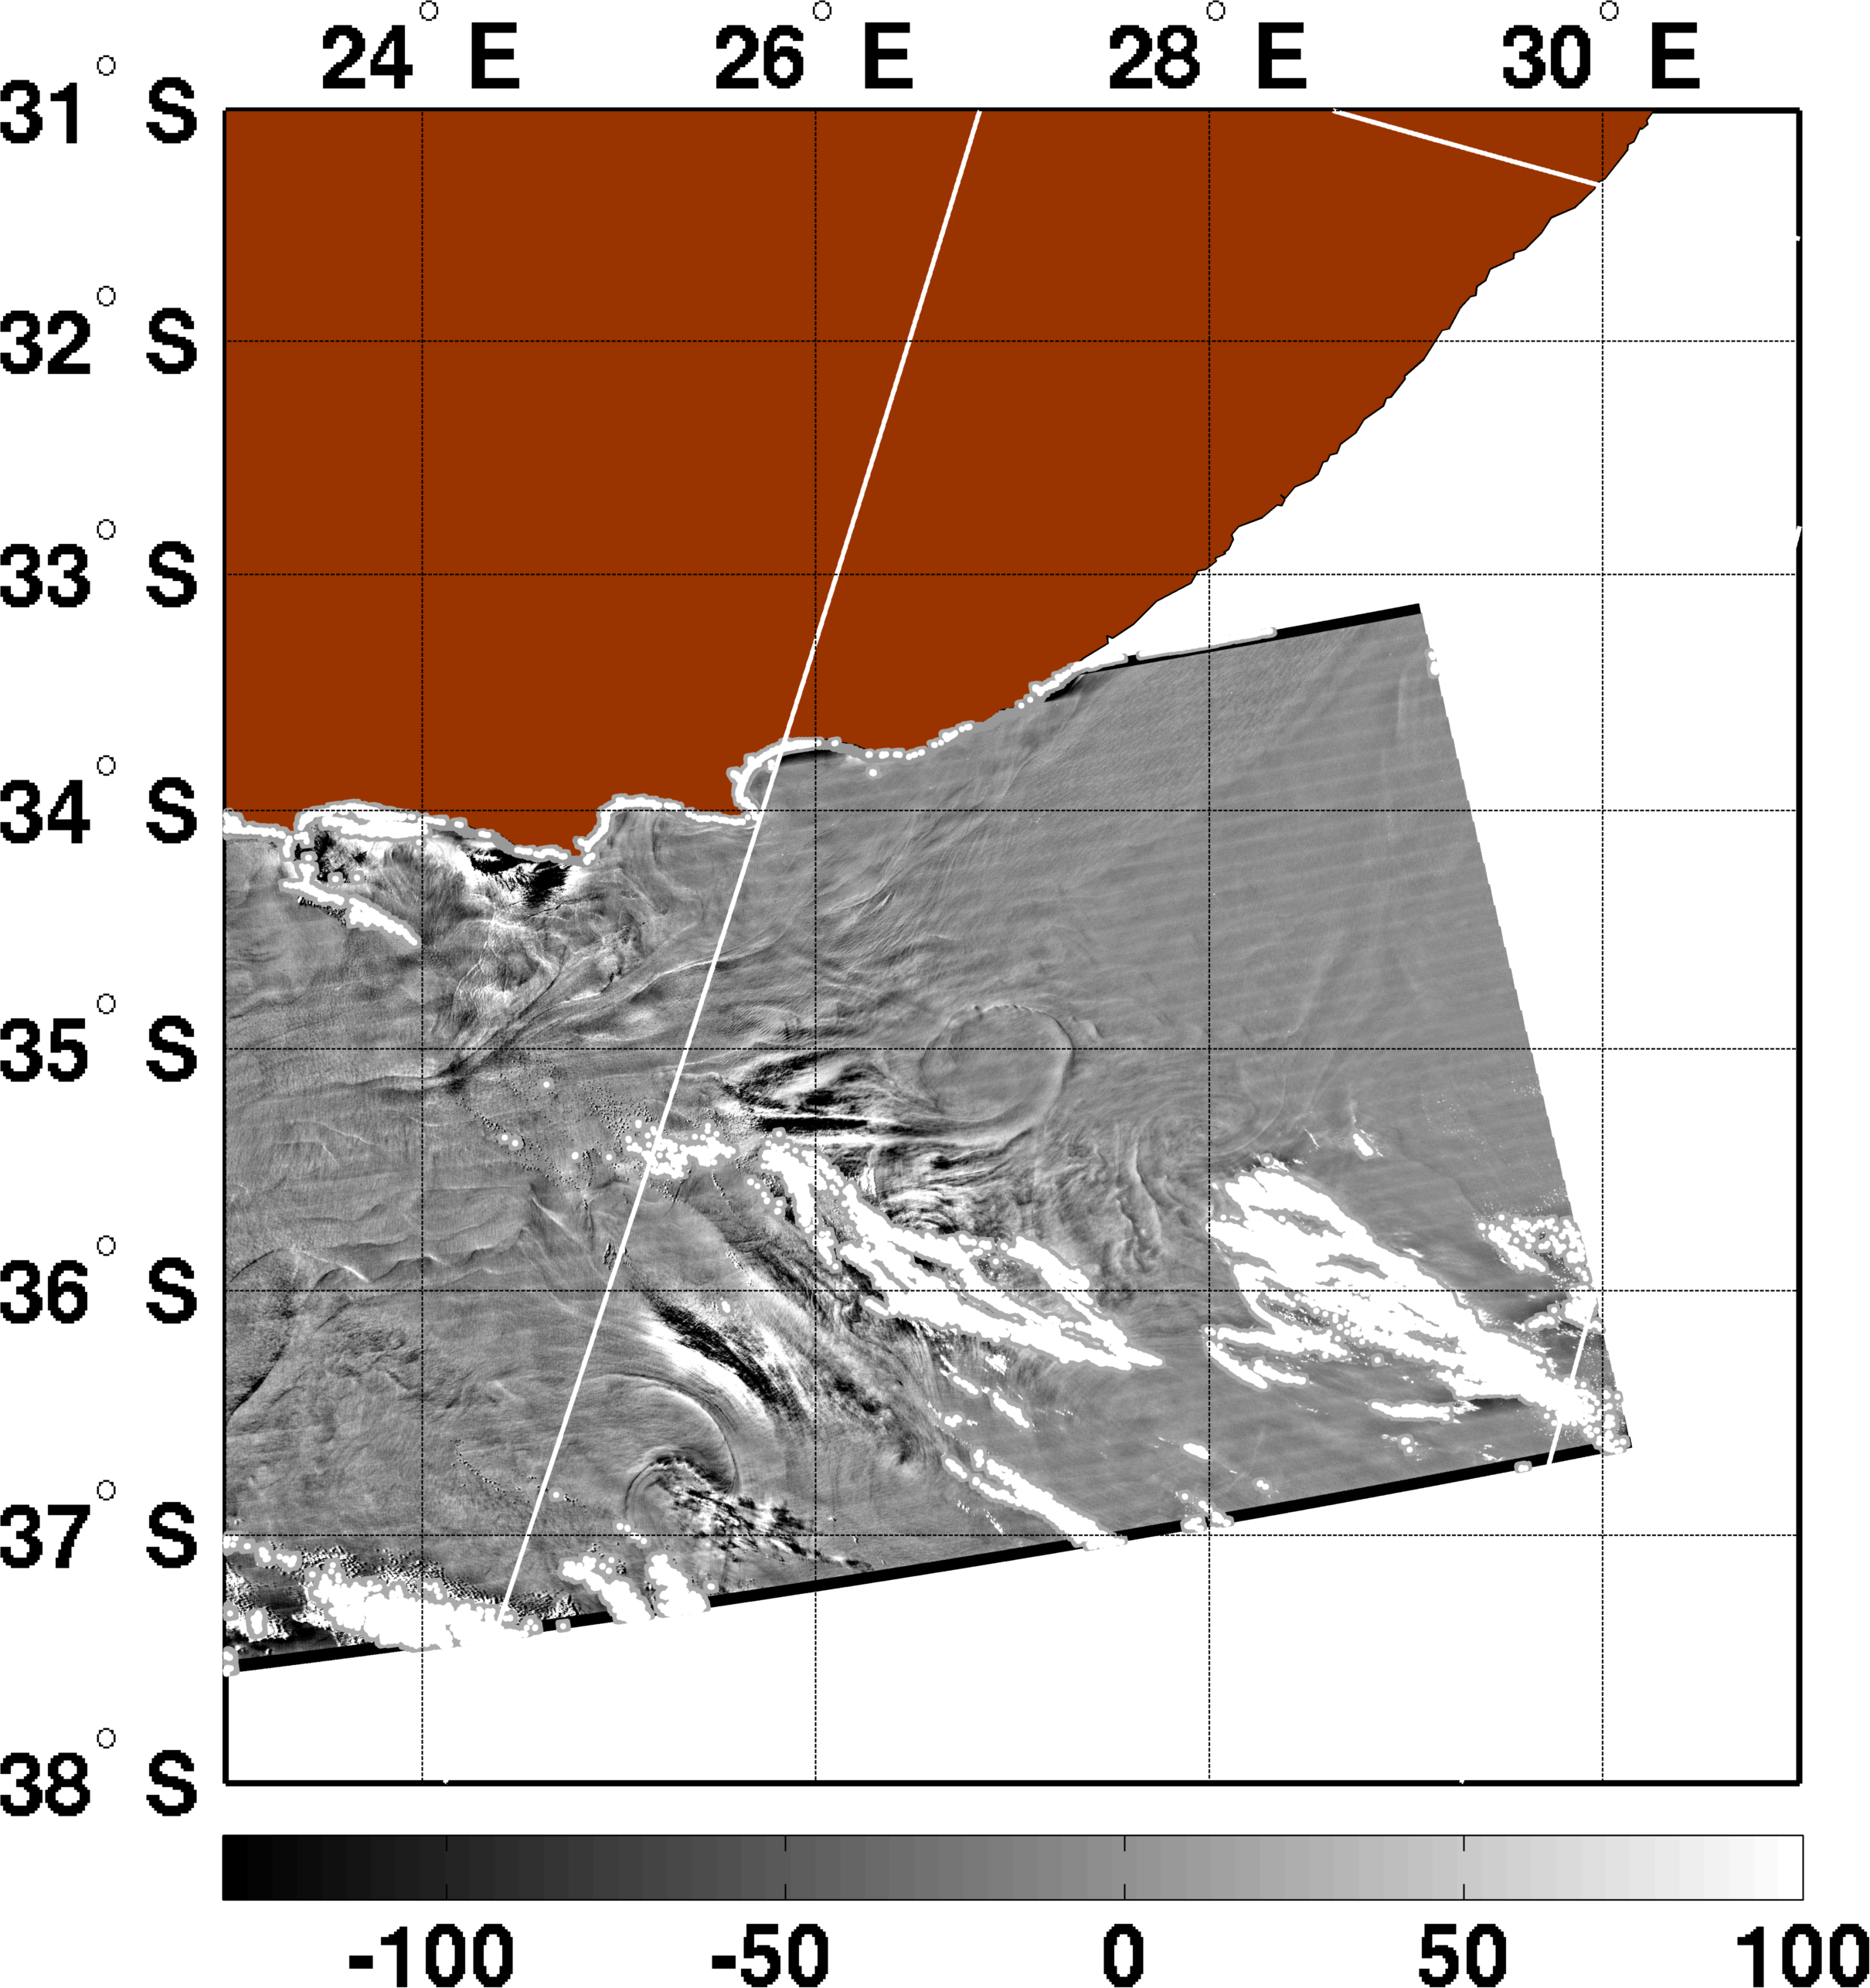
\includegraphics[width=1\linewidth]{fig3_4b}}
	\end{minipage}
    \\
    \floattitle{(а) Исходное изображение MODIS/Aqua района мыса Игольный, красный канал разрешением 250\textit{м}, полученное 18 Ноября 2007г., 12ч. 05мин. и вариации яркости (б). Обратите внимание на полосчатую структуру изображения MODIS, присущую снимкам областей солнечного блика, и особенно заметную на исходном изображении. Белые области -- маска облаков}
    \caption{Исходное изображение MODIS/Aqua района мыса Игольный и восстановленные контрасты СКН}
    \label{fig:3.4}
\end{figure}


На Рисунке~\ref{fig:3.5a} представлены контрасты СКН, полученные из вариаций яркости, приведённых на Рисунке~\ref{fig:3.4b}, с использованием передаточной функции \eqref{eq:1.7}. В поле СКН можно идентифицировать проявления фронтов, меандров и вихрей. Типичные значения амплитуды контрастов СКН, наблюдаемые на изображении, около 20-30\% с масштабами проявления структур от 1 до 10\textit{км}.



\begin{figure}[H]
   	\centering
	\begin{minipage}{.47\textwidth}
	    \subcaptionbox{\label{fig:3.5a}}
		{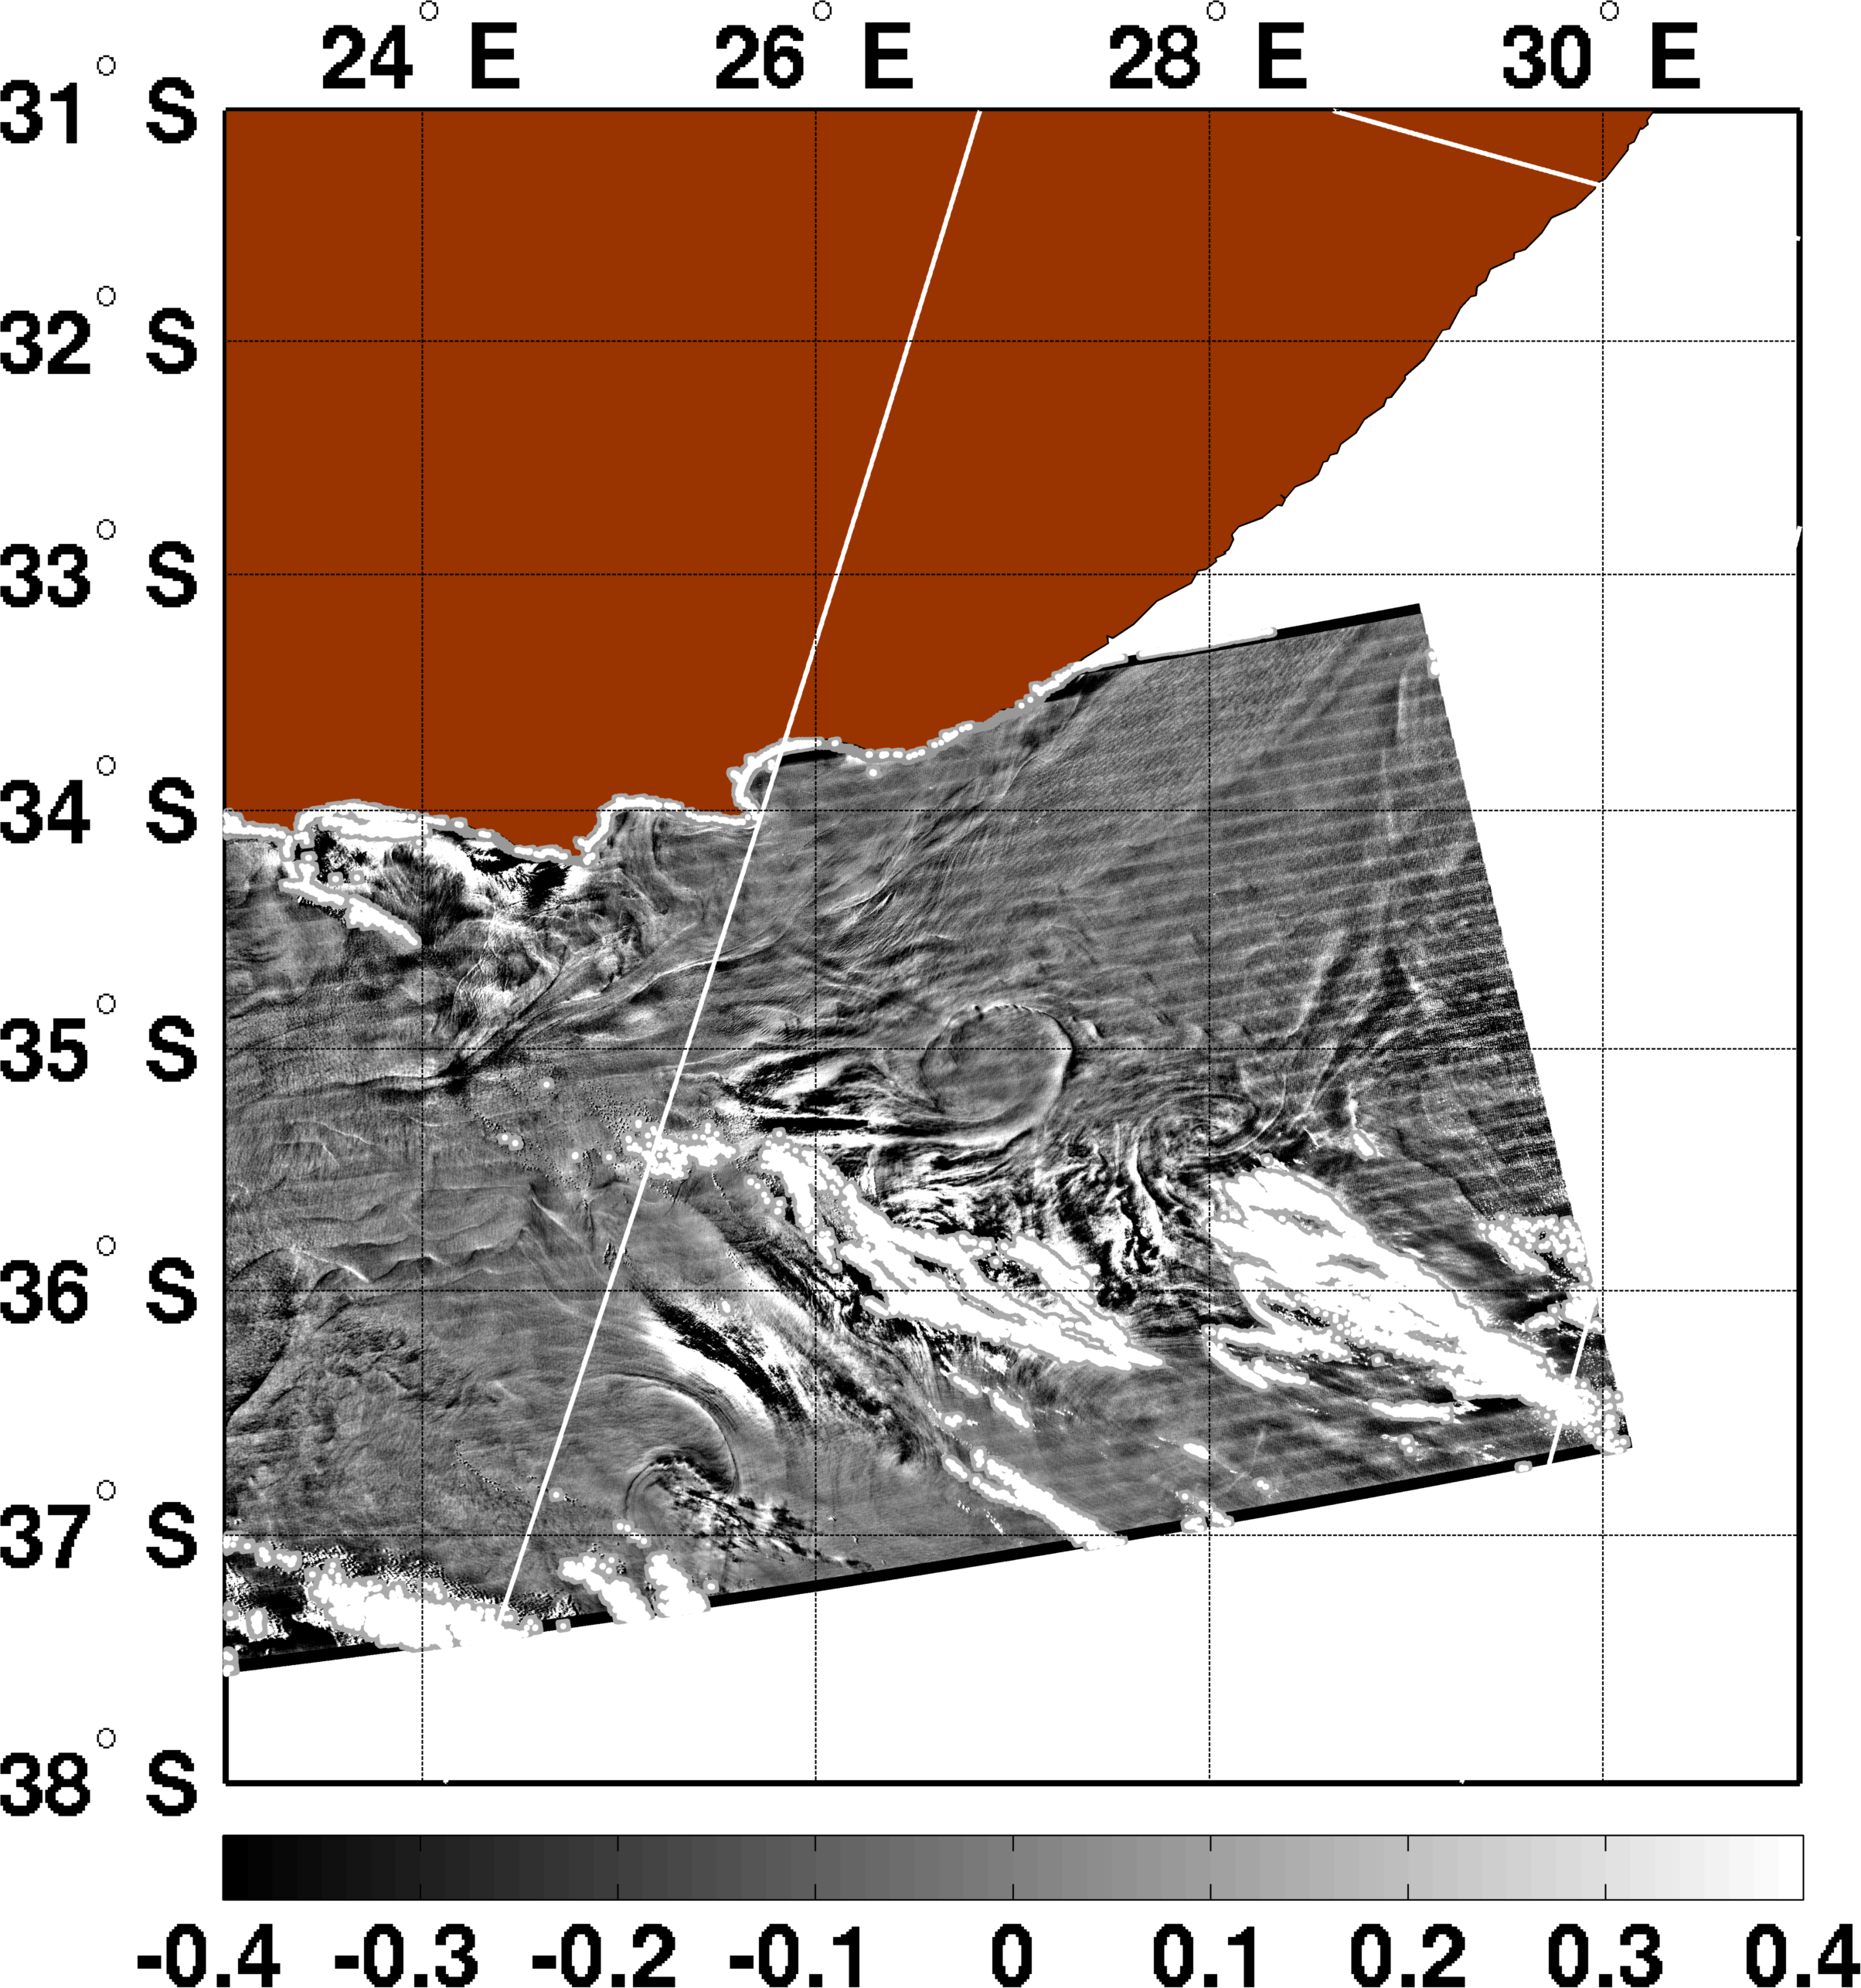
\includegraphics[width=1\linewidth]{fig3_5a}}
	\end{minipage}
	\hfill
	\begin{minipage}{.47\textwidth}
	    \subcaptionbox{\label{fig:3.5b}}
		{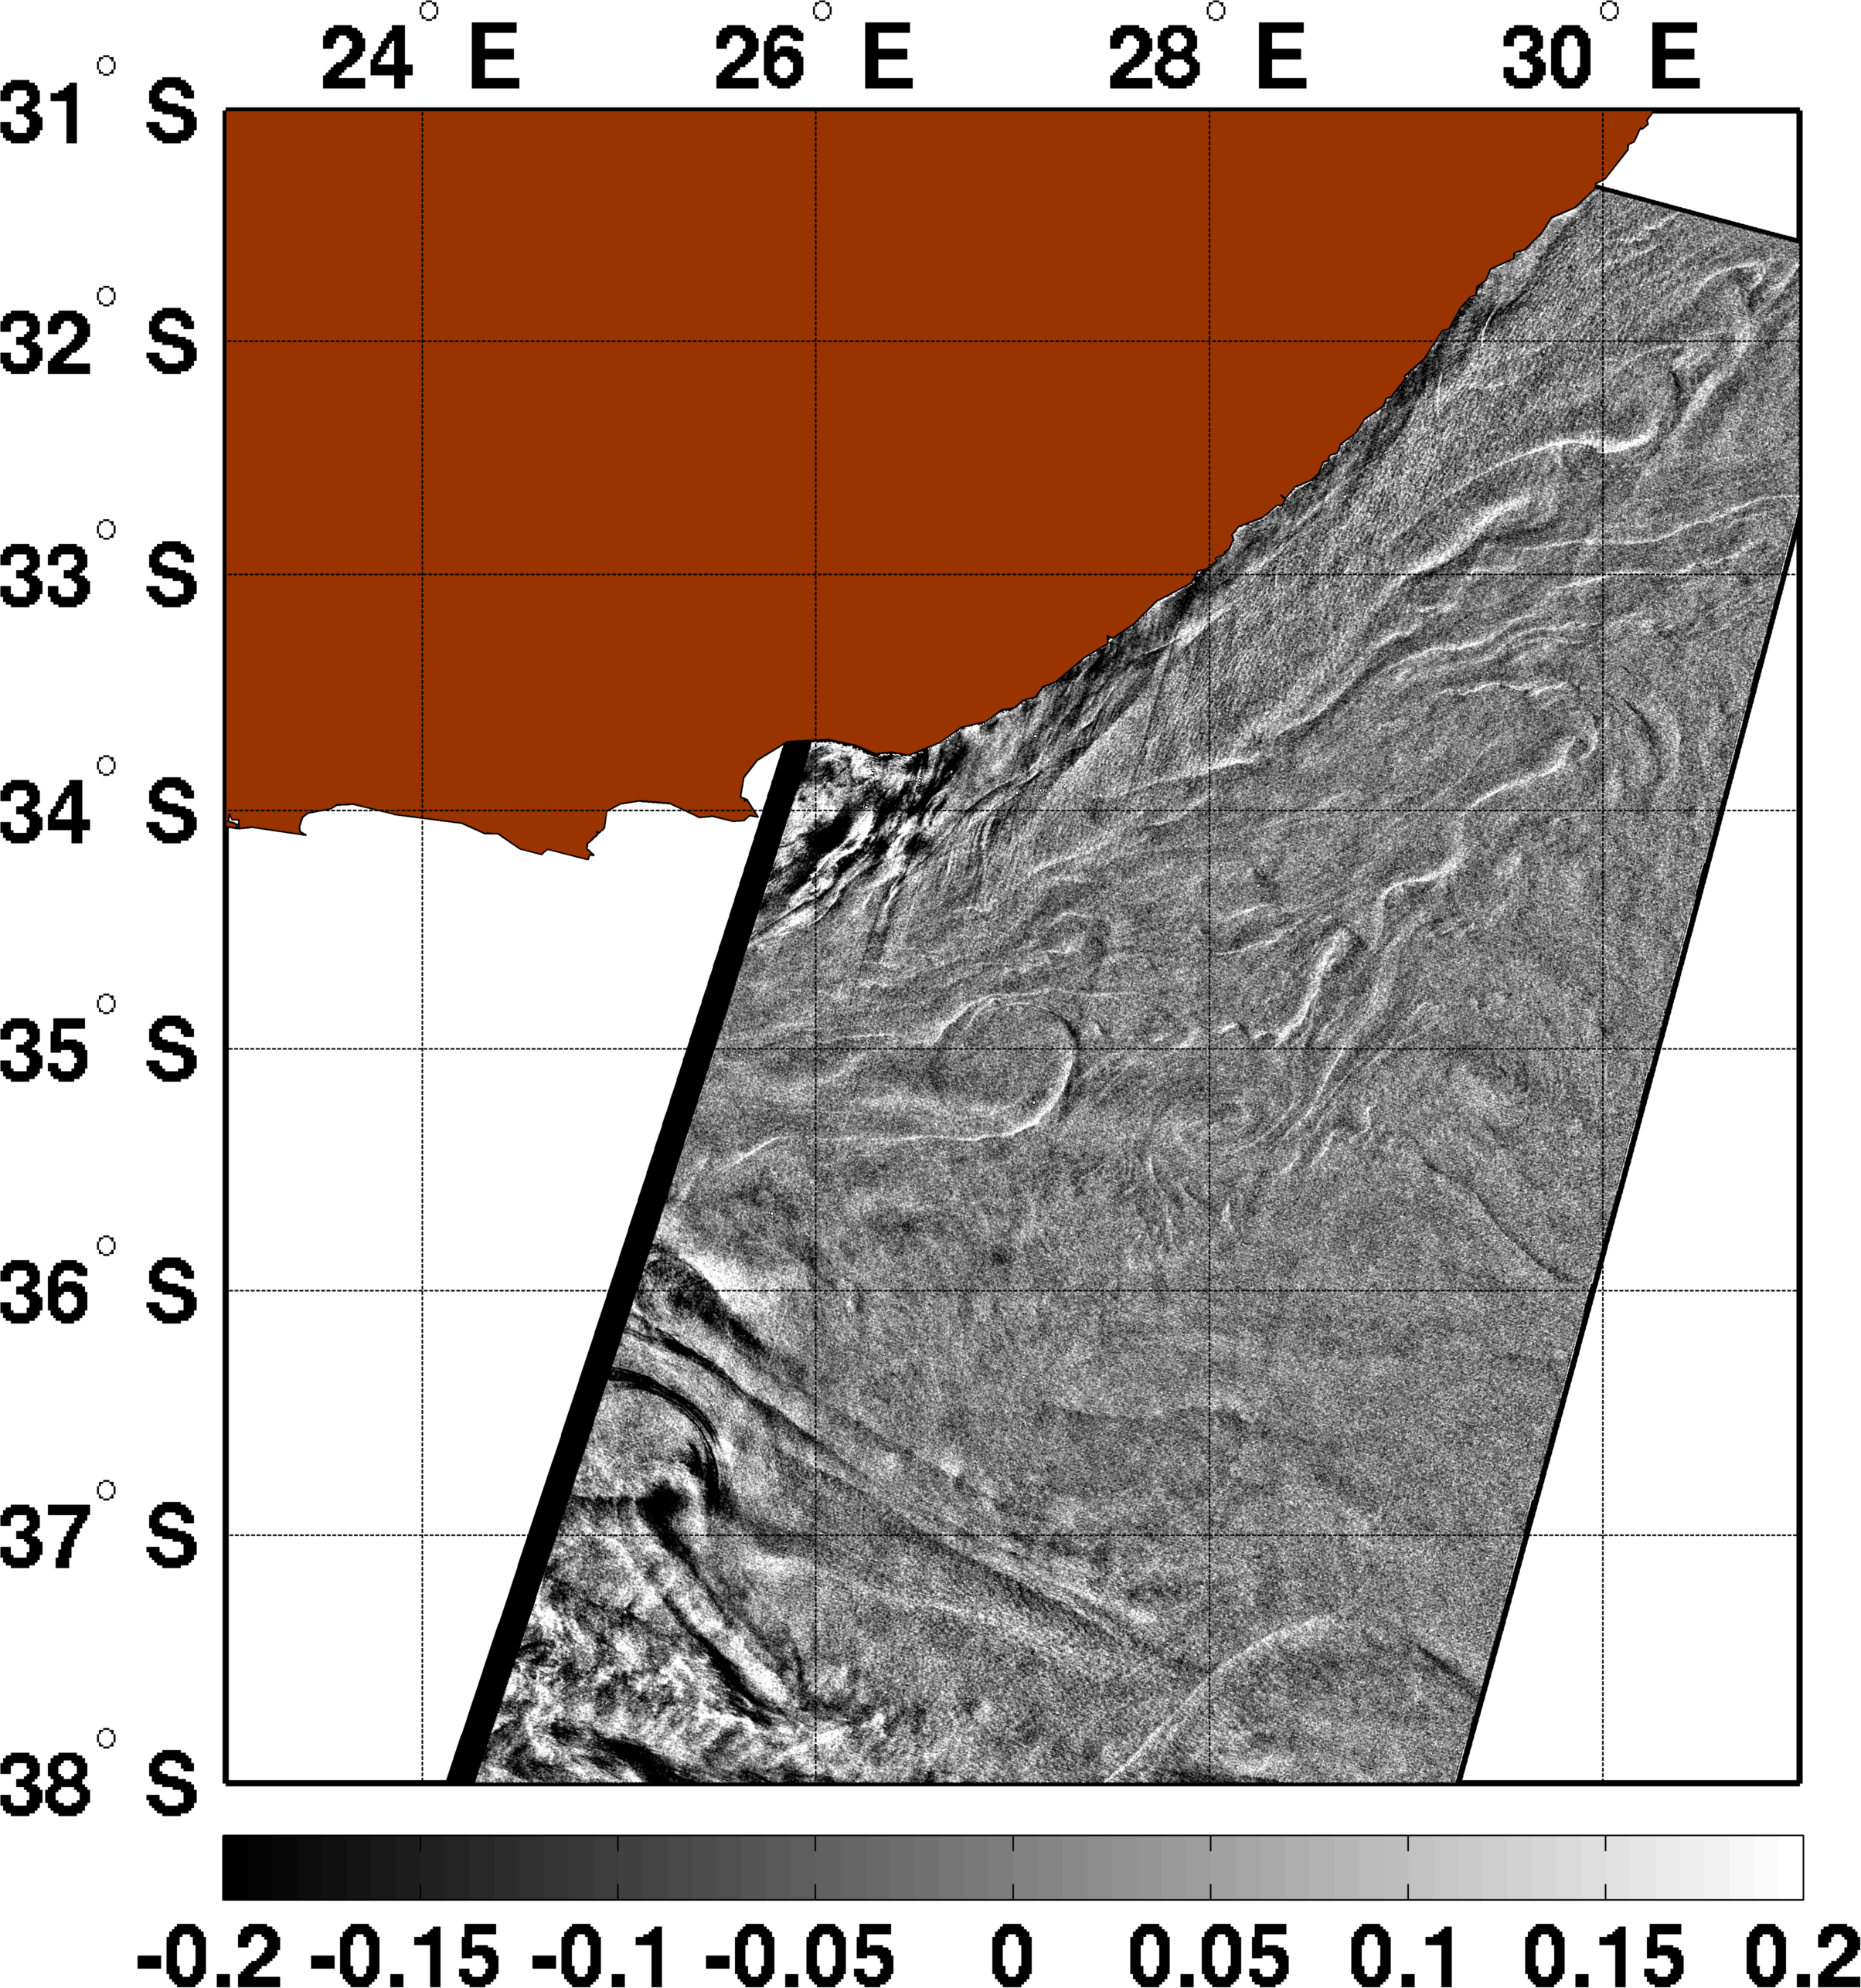
\includegraphics[width=1\linewidth]{fig3_5b}}
	\end{minipage}
    \\
    \caption{(а) Поле контрастов СКН, полученное из поля вариаций яркости, представленных на Рисунке~\ref{fig:3.4b} и поле контрастов УЭПР РСА (б)}
    \label{fig:3.5}
\end{figure}


Поле контрастов УЭПР РСА (Рисунок~\ref{fig:3.5b}), представлено как отношение разности исходного и усреднённого к среднему полю вариаций УЭПР, $K_{\sigma _{0} } =(\sigma _{0} -\overline{\sigma _{0} })/\overline{\sigma _{0} }$. Осреднение производилось скользящим средним с пространственным разрешением скользящего окна 30x30\textit{км${}^2$}. При сравнении поля контрастов СКН и поля контрастов УЭПР РСА можно заметить соответствие между двумя изображениями. В работе \citep{Johannessen2005} показано, что контрасты УЭПР на изображениях РСА отображают поле дивергенции поверхностного течения. Таким образом, подобие полей контрастов СКН и УЭПР РСА, позволяет утверждать, что поле контрастов СКН также отслеживает поле дивергенции поверхностного течения.



\subsection{Процедура реконструкции квазигеострофической и агеострофической циркуляции по ТПО} \label{sec:3.2.2}


Взаимодействие Экмановского потока с геострофическим течением является основным механизмом генерации вторичной агеострофической циркуляции (ВАЦ) в окрестности океанических фронтов \citep{Klein1990,Garrett1981,Thompson2000,Nagai2006}. Применим этот механизм для интерпретации проявлений температурных фронтов в шероховатости морской поверхности. Мы предполагаем, что полное поле океанического течения можно представить в виде суммы квазигеострофического течения (КГТ) ${\it U}$, ветрового течения ${\it u}^{e} $ (которое также может включать инерционное течение), и ВАЦ ${\it u}^{a} $, в результате взаимодействия Экмановского течения с КГТ и диабатического перемешивания в слое Экмана. Тогда уравнение для полного поля течения выражается как ${\it u=U+u}^{e} {\it +u}^{a} $.

В первом приближении по числу Россби, основные уравнения, описывающие динамику течения ВАЦ (подробнее см. \citep{Klein1990,Garrett1981,Thompson2000,Nagai2006}) представляются в виде:



\begin{equation} \label{eq:3.2} \begin{array}{l} {u_{\beta }^{e} \partial U_{1} /\partial x_{\beta } -fu_{2}^{a} =\nu _{t} \partial ^{2} U_{1} /\partial x_{3}^{2} } \\ {u_{\beta }^{e} \partial U_{2} /\partial x_{\beta } +fu_{1}^{a} =\nu _{t} \partial ^{2} U_{2} /\partial x_{3}^{2} } \end{array},  \end{equation} 



\noindent где $\nu _{t} $ - турбулентная вязкость, предполагается постоянной с глубиной (в верхнем перемешенном слое Экмана), $f$ - параметр Кориолиса, и $\beta =1,2$. В уравнении \eqref{eq:3.2} предполагается, что пространственный масштаб изменчивости ветрового поля намного превышает поперечный масштаб океанического фронта. С учётом выражения для ``термического ветра'': $\partial U_{1} /\partial x_{3} =(g/f)\partial \rho /\partial x_{2} $, $\partial U_{2} /\partial x_{3} =-(g/f)\partial \rho /\partial x_{1} $, и уравнения состояния Океана $\rho =\rho _{0} (1-\alpha T)$, решение уравнения \eqref{eq:3.2} для агеострофической компоненты течения имеет следующий вид:



\begin{equation} \label{eq:3.3} \begin{array}{l} {u_{1}^{a} =-f^{-1} u_{\beta }^{e} \frac{\partial U_{2} }{\partial x_{\beta } } +(\nu _{t} g\alpha /f^{2} )\frac{\partial }{\partial x_{3} } \left(\frac{\partial T}{\partial x_{1}^{} } \right)} \\ {u_{2}^{a} =f^{-1} u_{\beta }^{e} \frac{\partial U_{1} }{\partial x_{\beta } } +(\nu _{t} g\alpha /f^{2} )\frac{\partial }{\partial x_{3} } \left(\frac{\partial T}{\partial x_{2}^{} } \right)} \end{array},  \end{equation} 



\noindent где $g$ - ускорение свободного падения, а $\alpha $ - коэффициент термического расширения. Первый член в уравнении \eqref{eq:3.3} описывает генерацию ВАЦ в результате адвективного взаимодействия Экмановского течения с КГТ (механизм предложен \citep{Klein1990}), в то время как второй член учитывает фрикционный эффект в Экмановском слое (механизм описан \citep{Garrett1981}). Оба этих механизма приводят к возникновению дивергенции в окрестности термического фронта, что напрямую следует из уравнения. \eqref{eq:3.3}:



\begin{equation} \label{eq:3.4} \nabla \cdot {\it u}=-f^{-1} u_{\beta }^{e} \frac{\partial }{\partial x_{\beta } } \Omega +(\nu _{t} g\alpha /f^{2} )\frac{\partial }{\partial x_{3} } \Delta T,  \end{equation} 



\noindent где $\Omega _{z} =\partial U_{2} /\partial x_{1} -\partial U_{1} /\partial x_{2} \equiv \Delta \psi $ - завихренность КГТ, $\psi $ - функция тока и $\Delta T$ - Лапласиан поля поверхностной температуры. Соотношение л.ч. уравнения \eqref{eq:3.4} с первым членом его п.ч. представляет решение, полученное в \citep{Klein1990} для Экмановского адвективного механизма, а уравнение со вторым членом п.ч. уравнения \eqref{eq:3.4} -- решение \citep{Garrett1981}. для диабатического механизма перемешивания при генерации ВАЦ. Таким образом, уравнение \eqref{eq:3.4}, можно рассматривать как обобщённое решение, объединяющее оба механизма генерации агеострофической циркуляции в результате взаимодействия КГТ со слоем Экмана.

Далее предполагается, что ветровое течение представляется в виде суммы классической скорости течения Экмана ${\it u}^{ek} {\it =}\left[\tau _{2} /(fh),-\tau _{1} /(fh)\right]$ и скорости инерционного течения ${\it u}^{i} (t)$:



\begin{equation} \label{eq:3.5} {\it u}^{e} {\it =}\left[\tau _{2} /(fh),-\tau _{1} /(fh)\right]+{\it u}^{i} (t),  \end{equation} 



\noindent где ${\it \tau }=v_{*}^{2} [\cos \phi _{w} ,\sin \phi _{w} ]$, $v_{*} $ - динамическая скорость в воде, $\phi _{w} $ - направление вектора скорости ветра, $h=(\nu _{t} /f)^{1/2} $ - толщина Экмановского слоя, а ${\it u}^{i} (t)$ - инерционная скорость, которая может быть описана, используя временную изменчивость скорости ветра. Для определения выражения турбулентной вязкости $\nu _{t} $ будем использовать подобие морского и атмосферного пограничных (планетарных) слоёв. Для устойчиво стратифицированного пограничного слоя турбулентная вязкость $\nu _{t} =\gamma \kappa v_{*}^{} L$, где $\gamma \approx 0.2$ - постоянная, $\kappa \approx 0.4$ - постоянная Кармана, а $L$ - масштаб длины Обухова (см., например, \citep{Brown1982}). Выражая $L$ через частоту Брента-Вяйсяля для верхнего слоя Океана как $L=v_{*}^{3} /(\kappa v_{t} N^{2} )$, получаем турбулентную вязкость:



\begin{equation} \label{eq:3.6} \nu _{t} =\gamma ^{1/2} v_{*}^{2} /N,  \end{equation}



\noindent тогда глубина слоя Экмана:



\begin{equation} \label{eq:3.7} h=\gamma ^{1/4} v_{*} /\sqrt{fN} .  \end{equation} 



Оценка $h$ для скорости ветра 10\textit{м/с} и $f=10^{-4} $: $h\approx 28$\textit{м}, если соотношение Прандтля $N/f=10$, и $h\approx 90$\textit{м}, если $N/f=1$.

Чтобы дать определение дивергенции поверхностного течения (вызванную ВАЦ, в соответствии с уравнением \eqref{eq:3.4}), необходимо ввести поле КГТ. На мезомасштабах (10-500\textit{км}) и субмезомасштабах (1-10\textit{км}) динамика Океана такова, что, зачастую, в равновесно-стратифицированном, быстро вращающемся потоке, горизонтальные скорости, в среднем, значительно больше вертикальных. Таким образом, такое движение можно рассматривать как квази-двумерное, и его изучение проводить в рамках некоторых приближений. Основываясь на поверхностной квазигеострофической (ПКГ, от англ. surface quasi-geostrophic - SQG) динамике \citep{Held1995,Lapeyre2006}, Изерн-Фонтанет с коллегами \citep{Isern-Fontanet2008} предложили практический подход для восстановления поля скорости течения на масштабах от 30 до 300\textit{км} по изображению ТПО. Рассматривая ПКГ, функция тока КГТ $\widehat{\psi }({\it k},z)$ и поле ТПО $\widehat{T}_{s} ({\it k})$ в пространстве Фурье связаны следующим соотношением:



\begin{equation} \label{eq:3.8} \widehat{\psi }({\it k},z)=\frac{g\alpha \widehat{T}_{s} ({\it k})}{fn_{b} k} \exp (n_{0} kz),  \end{equation} 



\noindent где $n=N/f$ отношение Прандтля для частот Брента-Вяйсяля $N_{0} $ и $N_{b} $, определяющих, соответственно, мезо- и субмезомасштабные свойства потока. Определим скорость КГТ через функцию тока $\widehat{\psi }$, как $\widehat{{\it U}}=(-ik_{y} \widehat{\psi },ik_{x} \widehat{\psi })$ в пространстве Фурье, или в физическом пространстве ${\it U}=(-\partial \psi /\partial x_{2} ,\partial \psi /\partial x_{1} )$. Тогда, используя уравнение \eqref{eq:3.3}, возможно определить поле ВАЦ. 

В пространстве Фурье компоненты ВАЦ, определённые уравнениями \eqref{eq:3.3} и \eqref{eq:3.8} и дополненные оценками глубины слоя Экмана из уравнения \eqref{eq:3.7} и коэффициентом турбулентной вязкости из уравнения \eqref{eq:3.6}, выражаются через ТПО как:



\begin{equation} \label{eq:3.9} \left(\widehat{u_{1}^{a} },\widehat{u_{2}^{a} }\right){\rm =}\frac{\alpha }{\gamma ^{1/4} n_{b}^{1/2} } \cdot \frac{gv_{*} }{f^{2} } \left[s\cdot \sin (\phi _{w} -\phi )+i\gamma ^{3/4} n_{b}^{1/2} \frac{v_{*} K}{\left|f\right|} \right]\left(K_{1} ,K_{2} \right)\widehat{T}_{s} ,  \end{equation} 



\noindent где $s={\rm sign}(f)$, $i$ - мнимая единица, $\phi $ - направление вектора волнового числа ${\it K}$, и $\gamma =0.2$. Второй член в квадратных скобках отражает отношение механизмов перемешивания и адвекции. Если предположить, что $n_{b} =10$ и $f=10^{-4} $\textit{сек}$^{-1}$, тогда это отношение будет приблизительно равно 0.1 для скорости ветра 10\textit{м/с} и $K=2\pi /10^{4} $\textit{рад/м}. Для сравнения, это отношение приближается к единице для меньших масштабов, например, $K=2\pi /10^{3} $\textit{рад/м}. Эффективность механизма перемешивания возрастает как при уменьшении масштабов КГТ, так и при увеличении скорости ветра. Таким образом, при малых и умеренных скоростях ветра и масштабах течения порядка $K\propto 10^{-3} $\textit{рад/м} и меньших, механизм Экмановского переноса (который в общем случае также включает инерционные течения) доминирует над генерацией ВАЦ. Из уравнения \eqref{eq:3.9}, получаем выражение для дивергенции поверхностного течения в пространстве Фурье $\widehat{\nabla \cdot {\it u}}=iK_{\beta } \widehat{u_{\beta }^{a} }$:



\begin{equation} \label{eq:3.10} \widehat{\nabla \cdot {\it u}}{\rm =}\frac{i\alpha }{\gamma ^{1/4} n_{b}^{1/2} } \cdot \frac{gv_{*} }{f^{2} } \left[s\cdot \sin (\phi _{w} -\phi )+i\gamma ^{3/4} n_{b}^{1/2} \frac{v_{*} K}{\left|f\right|} \right]K^{2} \widehat{T}_{s} .  \end{equation} 



В результате перед нами уравнение, напрямую связывающее дивергенцию поверхностного течения с полем ТПО.



\subsection{Особенности мезомасштабных течений, восстановленные по ТПО, и их связь с аномалиями РСА сигнала и СКН} \label{sec:3.2.3}
 

Сравним контрасты СКН и УЭПР РСА, показанные на Рисунке~\ref{fig:3.5}, с проявлениями различных океаническиз явлений в поле ТПО, представленном на Рисунке~\ref{fig:3.3}. Уже при беглом осмотре можно заметить поразительное соответствие этих полей. Изменения полей контрастов СКН и УЭПР совпадают с локальными изменениями в поле ТПО. В принципе, наблюдаемое соответствие дожны восхищать, но не должны удивлять, поскольку известно, что океанические фронтальные зоны характеризуются интенсивными перекрестными фронтальными и вертикальными движениями (апвеллинг/даунвеллинг). В этом контексте, может быть использована модель восстановления поля поверхностных течений по изображению поля ТПО, описанная в предыдущем разделе, в качестве экспериментального свидетельства связи аномалий шероховатости морской поверхности и полем дивергенции течения.

Поле ТПО, полученное по данным прибора MODIS (см. Рисунок~\ref{fig:3.3b} ) и поле, восстановленного по данным РСА, ветра (см. Рисунок~\ref{fig:3.3a} ) используются в качестве входных параметров для нахождения поля скорости поверхностного течения. Поскольку описанный в предыдущем разделе алгоритм воостановления поверхностного КГТ применим на масштабах 30-300\textit{км} спектральные компоненты с $K<2\pi /100$\textit{рад/км} были отсечены. Компоненты течения находятся из функции тока КГТ, определенного из уравнения \eqref{eq:3.8}. Чтобы получить низкое стандартное отклонение полученных скоростей КГТ (около 1\textit{м/с}) предполагалось, что $n_{b} =n_{0} =50$. Использование этих констант также помогает сравнивать полученные по РСА поверхностные скорости \citep{Chapron2005, Johannessen2008} с измерениями Доплеровских сдвигов по дальности (не показано здесь). Фоновое Экмановское течение (\eqref{eq:3.5}) и ВАЦ (\eqref{eq:3.3}), рассчитаны для усреднённого наблюдаемого ветра  7\textit{м/с} южного по направлению.

Завихренность поля КГТ и дивергенция поверхностного течения, восстановленные по наблюдаемому полю ТПО, показаны на Рисунке~\ref{fig:3.6}. Поле завихренности КГТ демонстрирует разнообразие мезомасштабных явлений на поверхности Океана (меандрирующие фронты, вихревые образования и прочее), а также наличие ``основной струи'', представляющей течение мыса Игольный. Если сравнить поле завихренности Рисунок~\ref{fig:3.6a} с дивергенцией поверхностного течения Рисунок~\ref{fig:3.6b}, видно, что области смены знака в поле конвергенции/дивергенции повторяют градиенты поля завихренности КГТ, которое, исходя из уравнения \eqref{eq:3.10}, связано с полем Лапласиана ТПО.



\begin{figure}[H]
   	\centering
	\begin{minipage}{.47\textwidth}
	    \subcaptionbox{\label{fig:3.6a}}
		{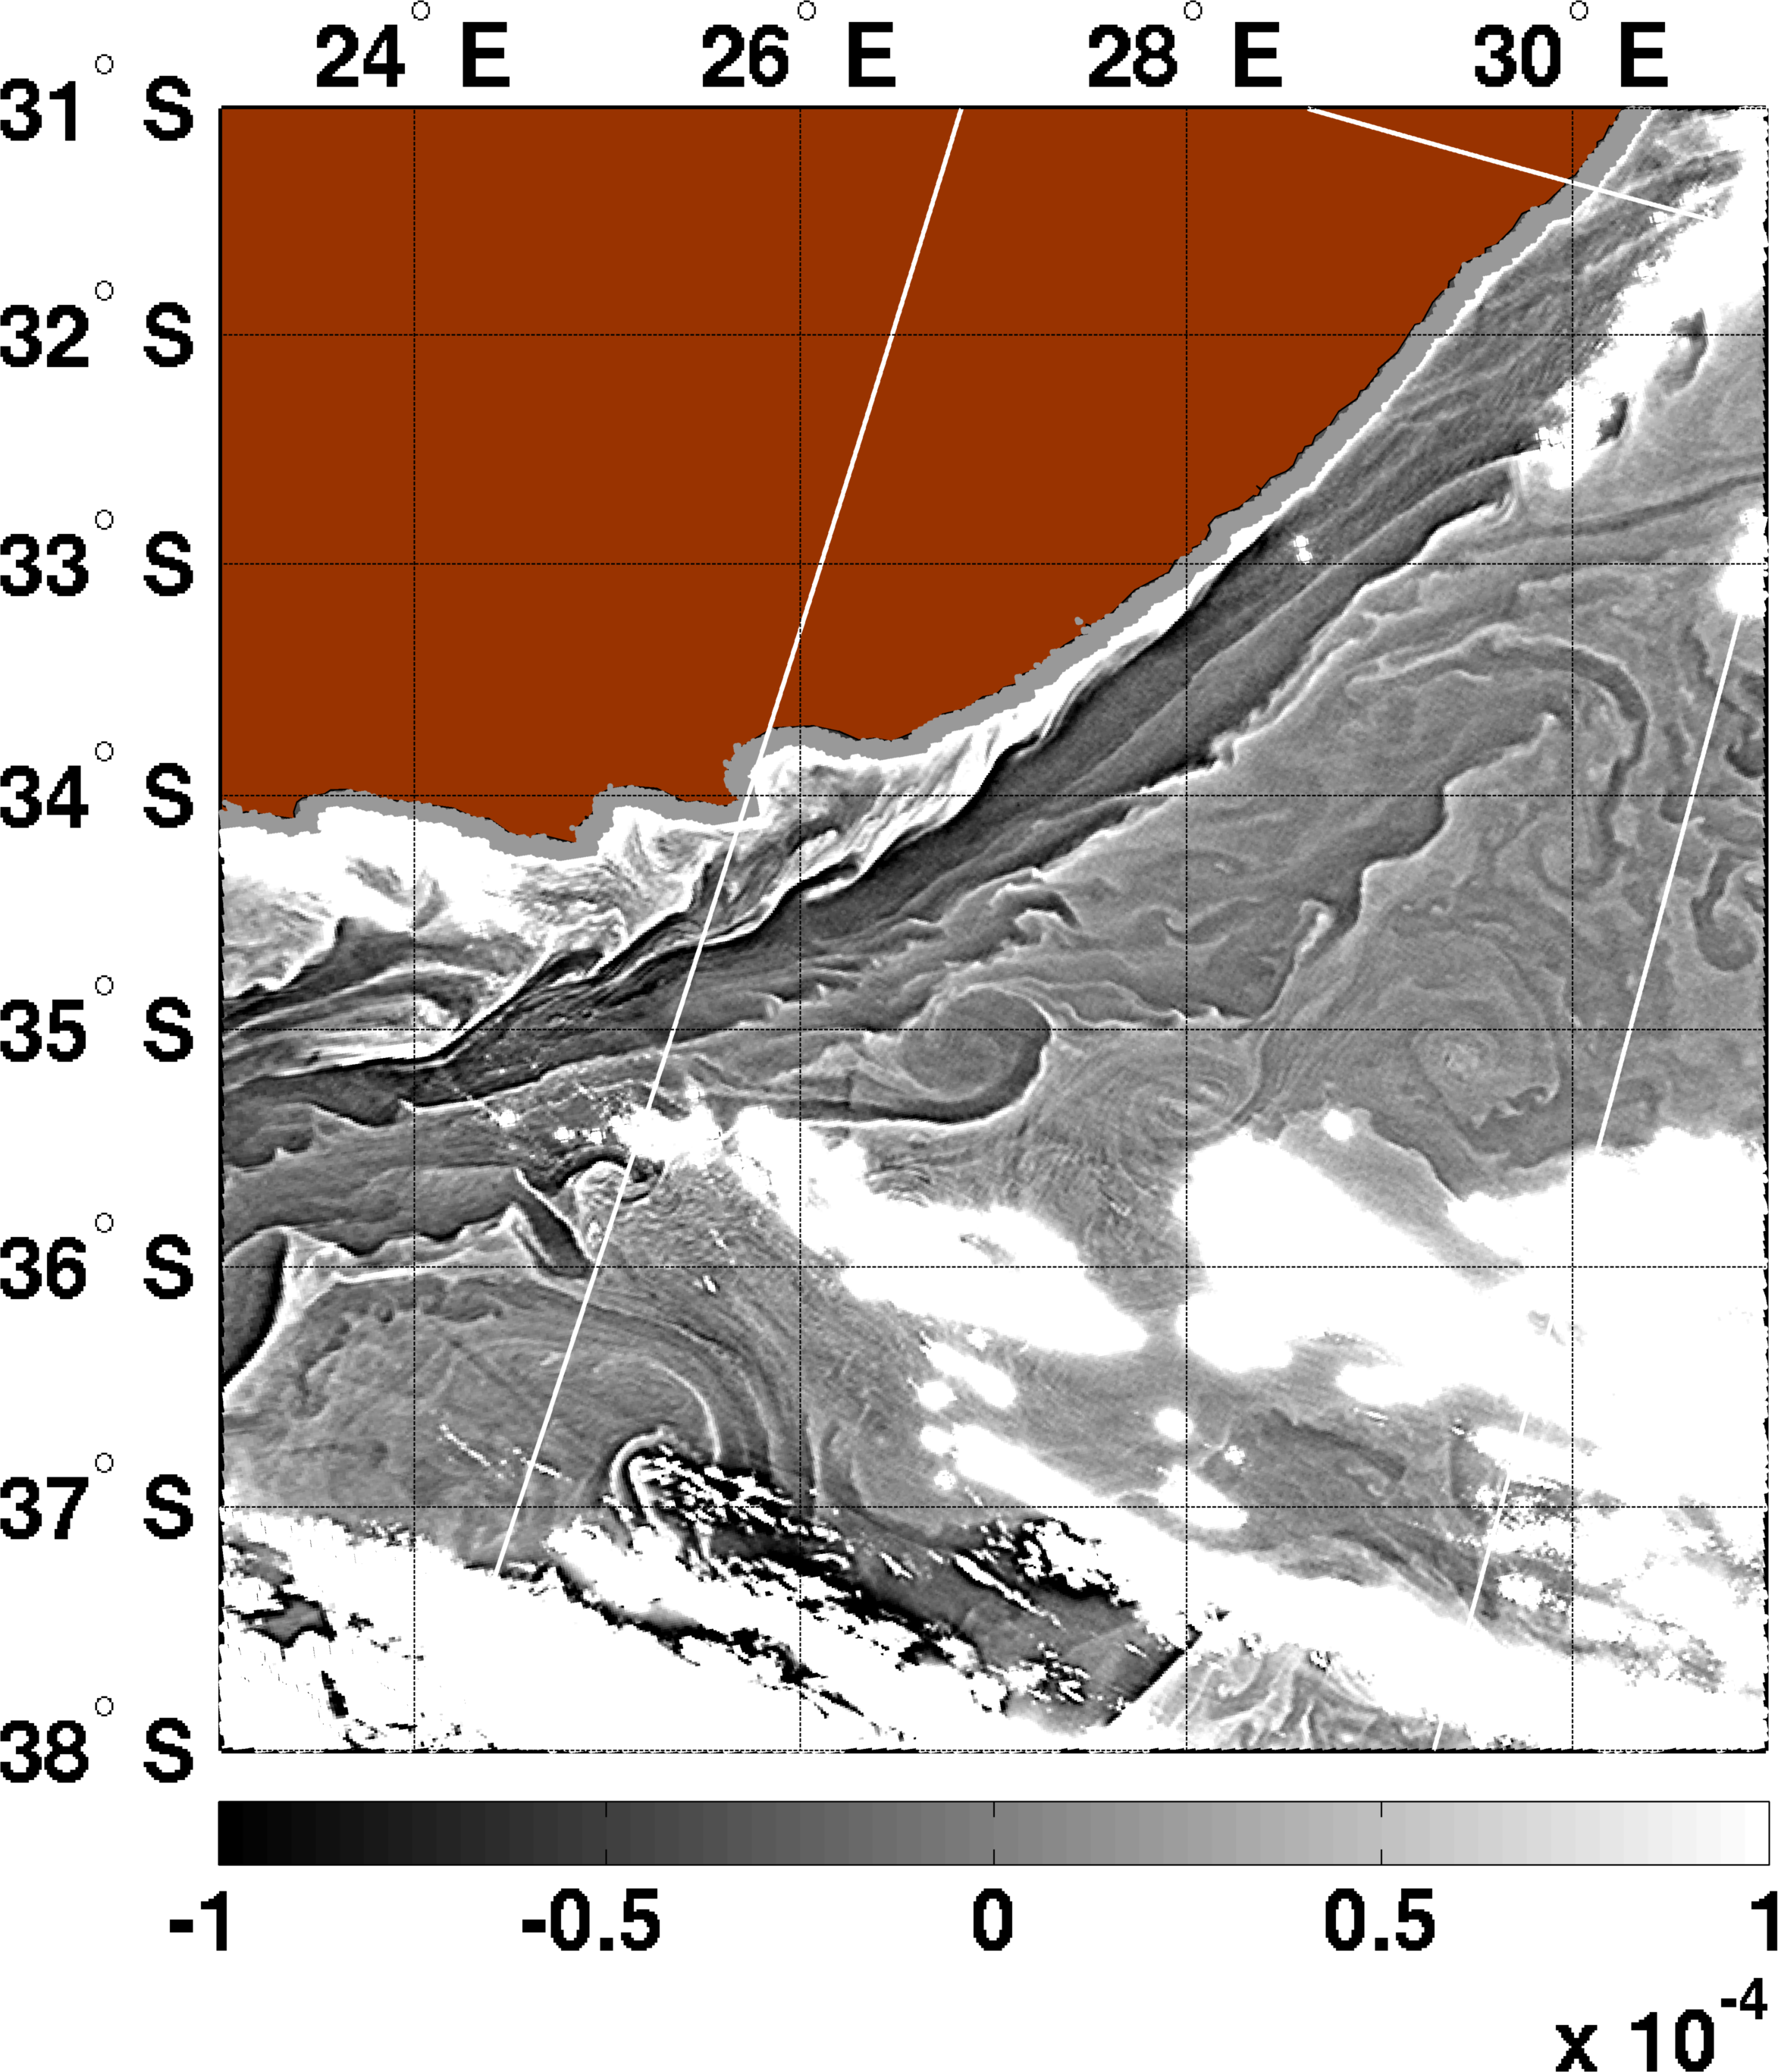
\includegraphics[width=1\linewidth]{fig3_6a}}
	\end{minipage}
	\hfill
	\begin{minipage}{.47\textwidth}
	    \subcaptionbox{\label{fig:3.6b}}
		{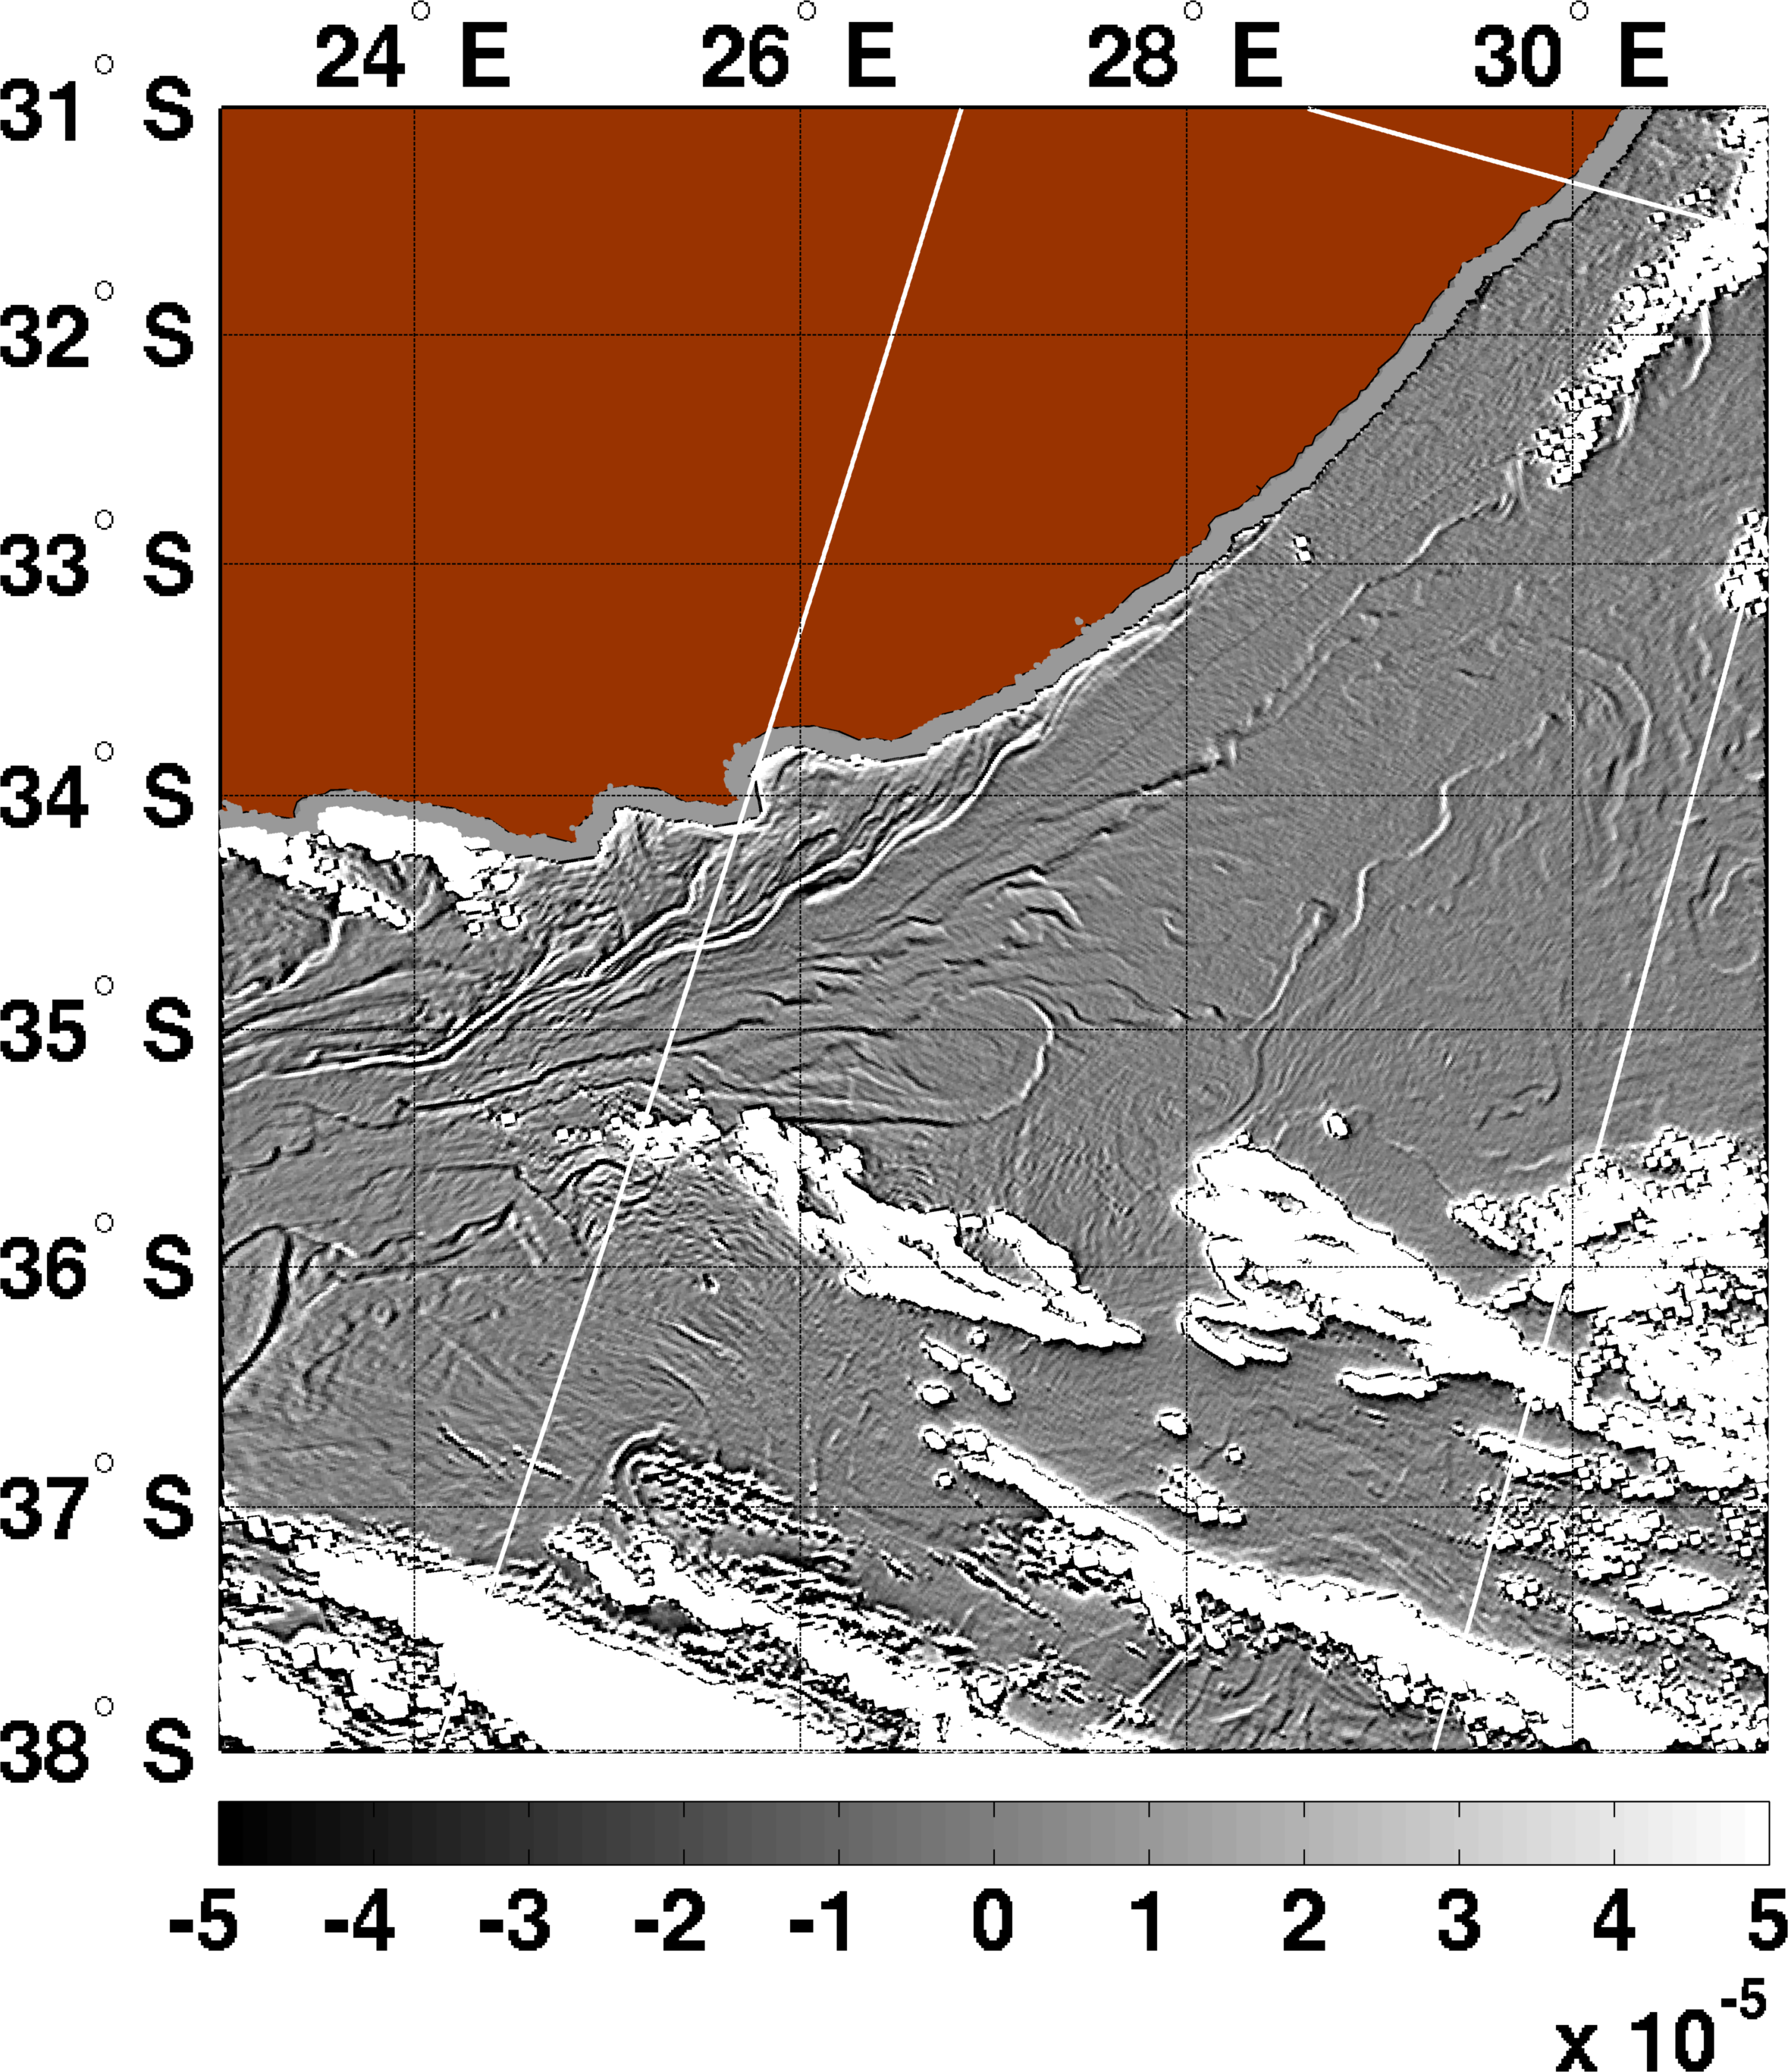
\includegraphics[width=1\linewidth]{fig3_6b}}
	\end{minipage}
    \\
    \floattitle{(а) Завихренность поверхностного квазигеострофического течения (КГТ), полученное по полю ТПО, показанному на Рисунке~\ref{fig:3.3b} , используя уравнение. (б) Поле поверхностной дивергенции, $\nabla \cdot {\it u}$, относящееся ко вторичной агеострофической циркуляции, образующейся в результате взаимодействия Экмановской накачки (адвективный и механизм перемешивания) с КГТ (см. уравнения \eqref{eq:3.4} и \eqref{eq:3.10}). Стоит отметить, что поле дивергенции инвертировано (показано поле $-\nabla \cdot {\it u}$). Таким образом, яркие объекты на изображении соответствуют зонам конвергенции, а тёмные -- зонам дивергенции}
    \caption{Завихренность поля КГТ и дивергенция поверхностного течения, восстановленные по наблюдаемому полю ТПО}
    \label{fig:3.6}
\end{figure}


На фрагменте РСА изображения (Рисунок~\ref{fig:3.7a}) наблюдаемые контрасты УЭПР РСА возможно являются поверхностными проявлениями мезомасштабной динамики Океана, поскольку поле ветра в этом районе однородно (см. Рисунок~\ref{fig:3.5}), т.е. нет вариаций ветра, способных привести к вариациям шероховатости морской поверхности. а следовательно и изменениям контрастов УЭПР. Соответствующее поле дивергенции поверхностного течения представлено на Рисунке~\ref{fig:3.7b}.



\begin{figure}[H]
   	\centering
	\begin{minipage}{.47\textwidth}
	    \subcaptionbox{\label{fig:3.7a}}
		{\includegraphics[width=1\linewidth]{fig3_7a}}
	\end{minipage}
	\hfill
	\begin{minipage}{.47\textwidth}
	    \subcaptionbox{\label{fig:3.7b}}
		{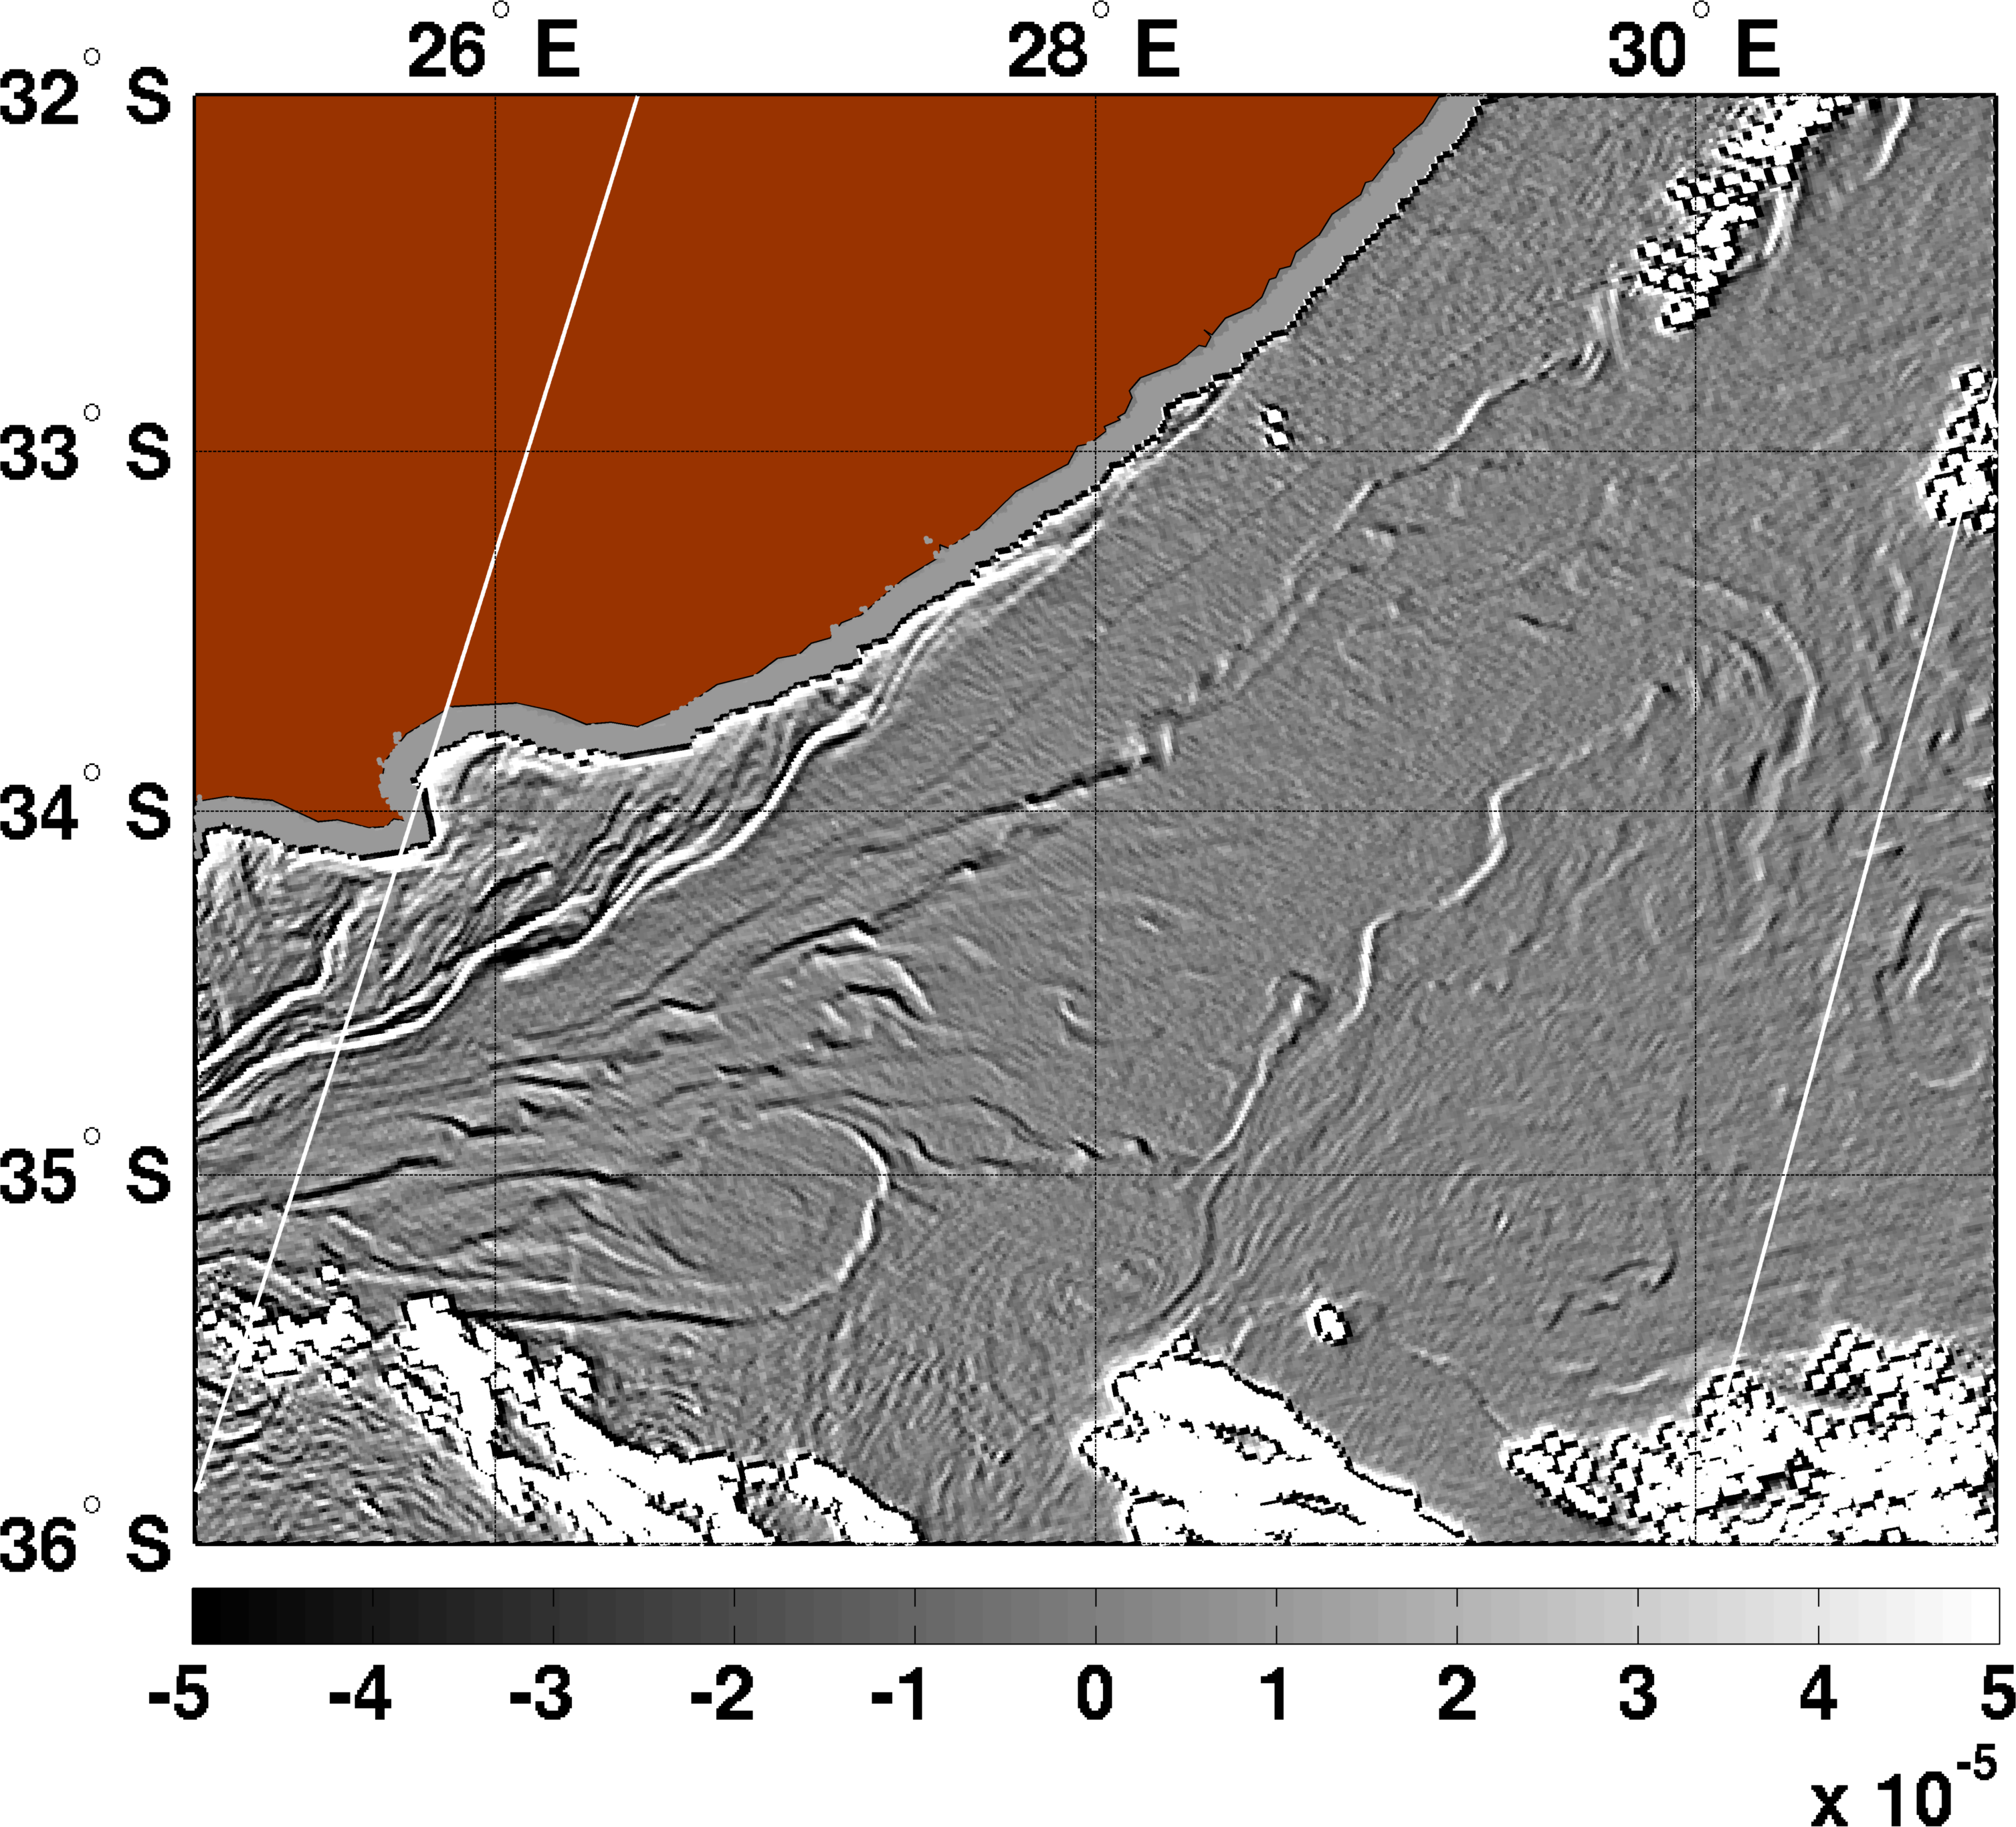
\includegraphics[width=1\linewidth]{fig3_7b}}
	\end{minipage}
    \\
    \floattitle{(а) Фрагмент поля УЭПР РСА, показанный ранее на Рисунке~\ref{fig:3.5}, и (б) соответствующий фрагмент поля дивергенции поверхностного течения, показанного на Рисунке~\ref{fig:3.6}. Яркие области на рисунке (б) соответствуют конвергенции течения, а тёмные -- дивергенции (детальнее см. подпись к Рисунку~\ref{fig:3.6})}
    \caption{Фрагменты поля УЭПР РСА и дивергенции поверхностного течения}
    \label{fig:3.7}
\end{figure}


При детальном рассмотрении Рисунка~\ref{fig:3.7} можно увидеть, что поля контрастов УЭПР и дивергенции имеют очень похожие текстуры. При этом не стоит забывать о 5-и часовой разнице при получении изображениями ASAR и MODIS. Из Рисунка~\ref{fig:3.7} следует, что яркие контрасты УЭПР соответствуют зонам конвергенции течения, в то время как тёмные контрасты представляют области дивергенции. Более того, это наблюдение можно рассматривать как экспериментальное подтверждение модельных открытий, представленных в работах \citep{Kudryavtsev2005,Johannessen2005}, и, упрощенных в уравнениях \eqref{eq:1.5}, \eqref{eq:1.7}, \eqref{eq:1.8} и \eqref{eq:1.9}. Также, если существует связь между аномалиями УЭПР и дивергенцией течения, то явное хорошее соответствие между отклонениями РСА контрастов и полем дивергенции поверхностного течения означает, что наш подход для восстановления КГТ и ВАЦ работает должным образом и дает правдоподобные оценки поля поверхностного течения.

Аналогичный вывод может быть сделан для фрагмента поля контрастов СКН, изображенного на Рисунке~\ref{fig:3.8a} (увеличенный фрагмент поля СКН, представленного на Рисунке~\ref{fig:3.5}). Поле дивергенции на Рисунке~\ref{fig:3.8b} восстановлено по ТПО для северного ветра, чтобы соответствовать контрастам СКН. Стоит отметить, что направление ветра для этого рисунка противоположно выбранному для расчётов поля дивергенции, показанного на Рисунке~\ref{fig:3.6b}. Исходя из уравнения \eqref{eq:3.10}, следует, что направление ветра влияет на знак $\nabla \cdot {\it u}$, что объясняет различие с соответствующим фрагментом, изображенным на Рисунке~\ref{fig:3.6b}.



\begin{figure}[H]
   	\centering
	\begin{minipage}{.47\textwidth}
	    \subcaptionbox{\label{fig:3.8a}}
		{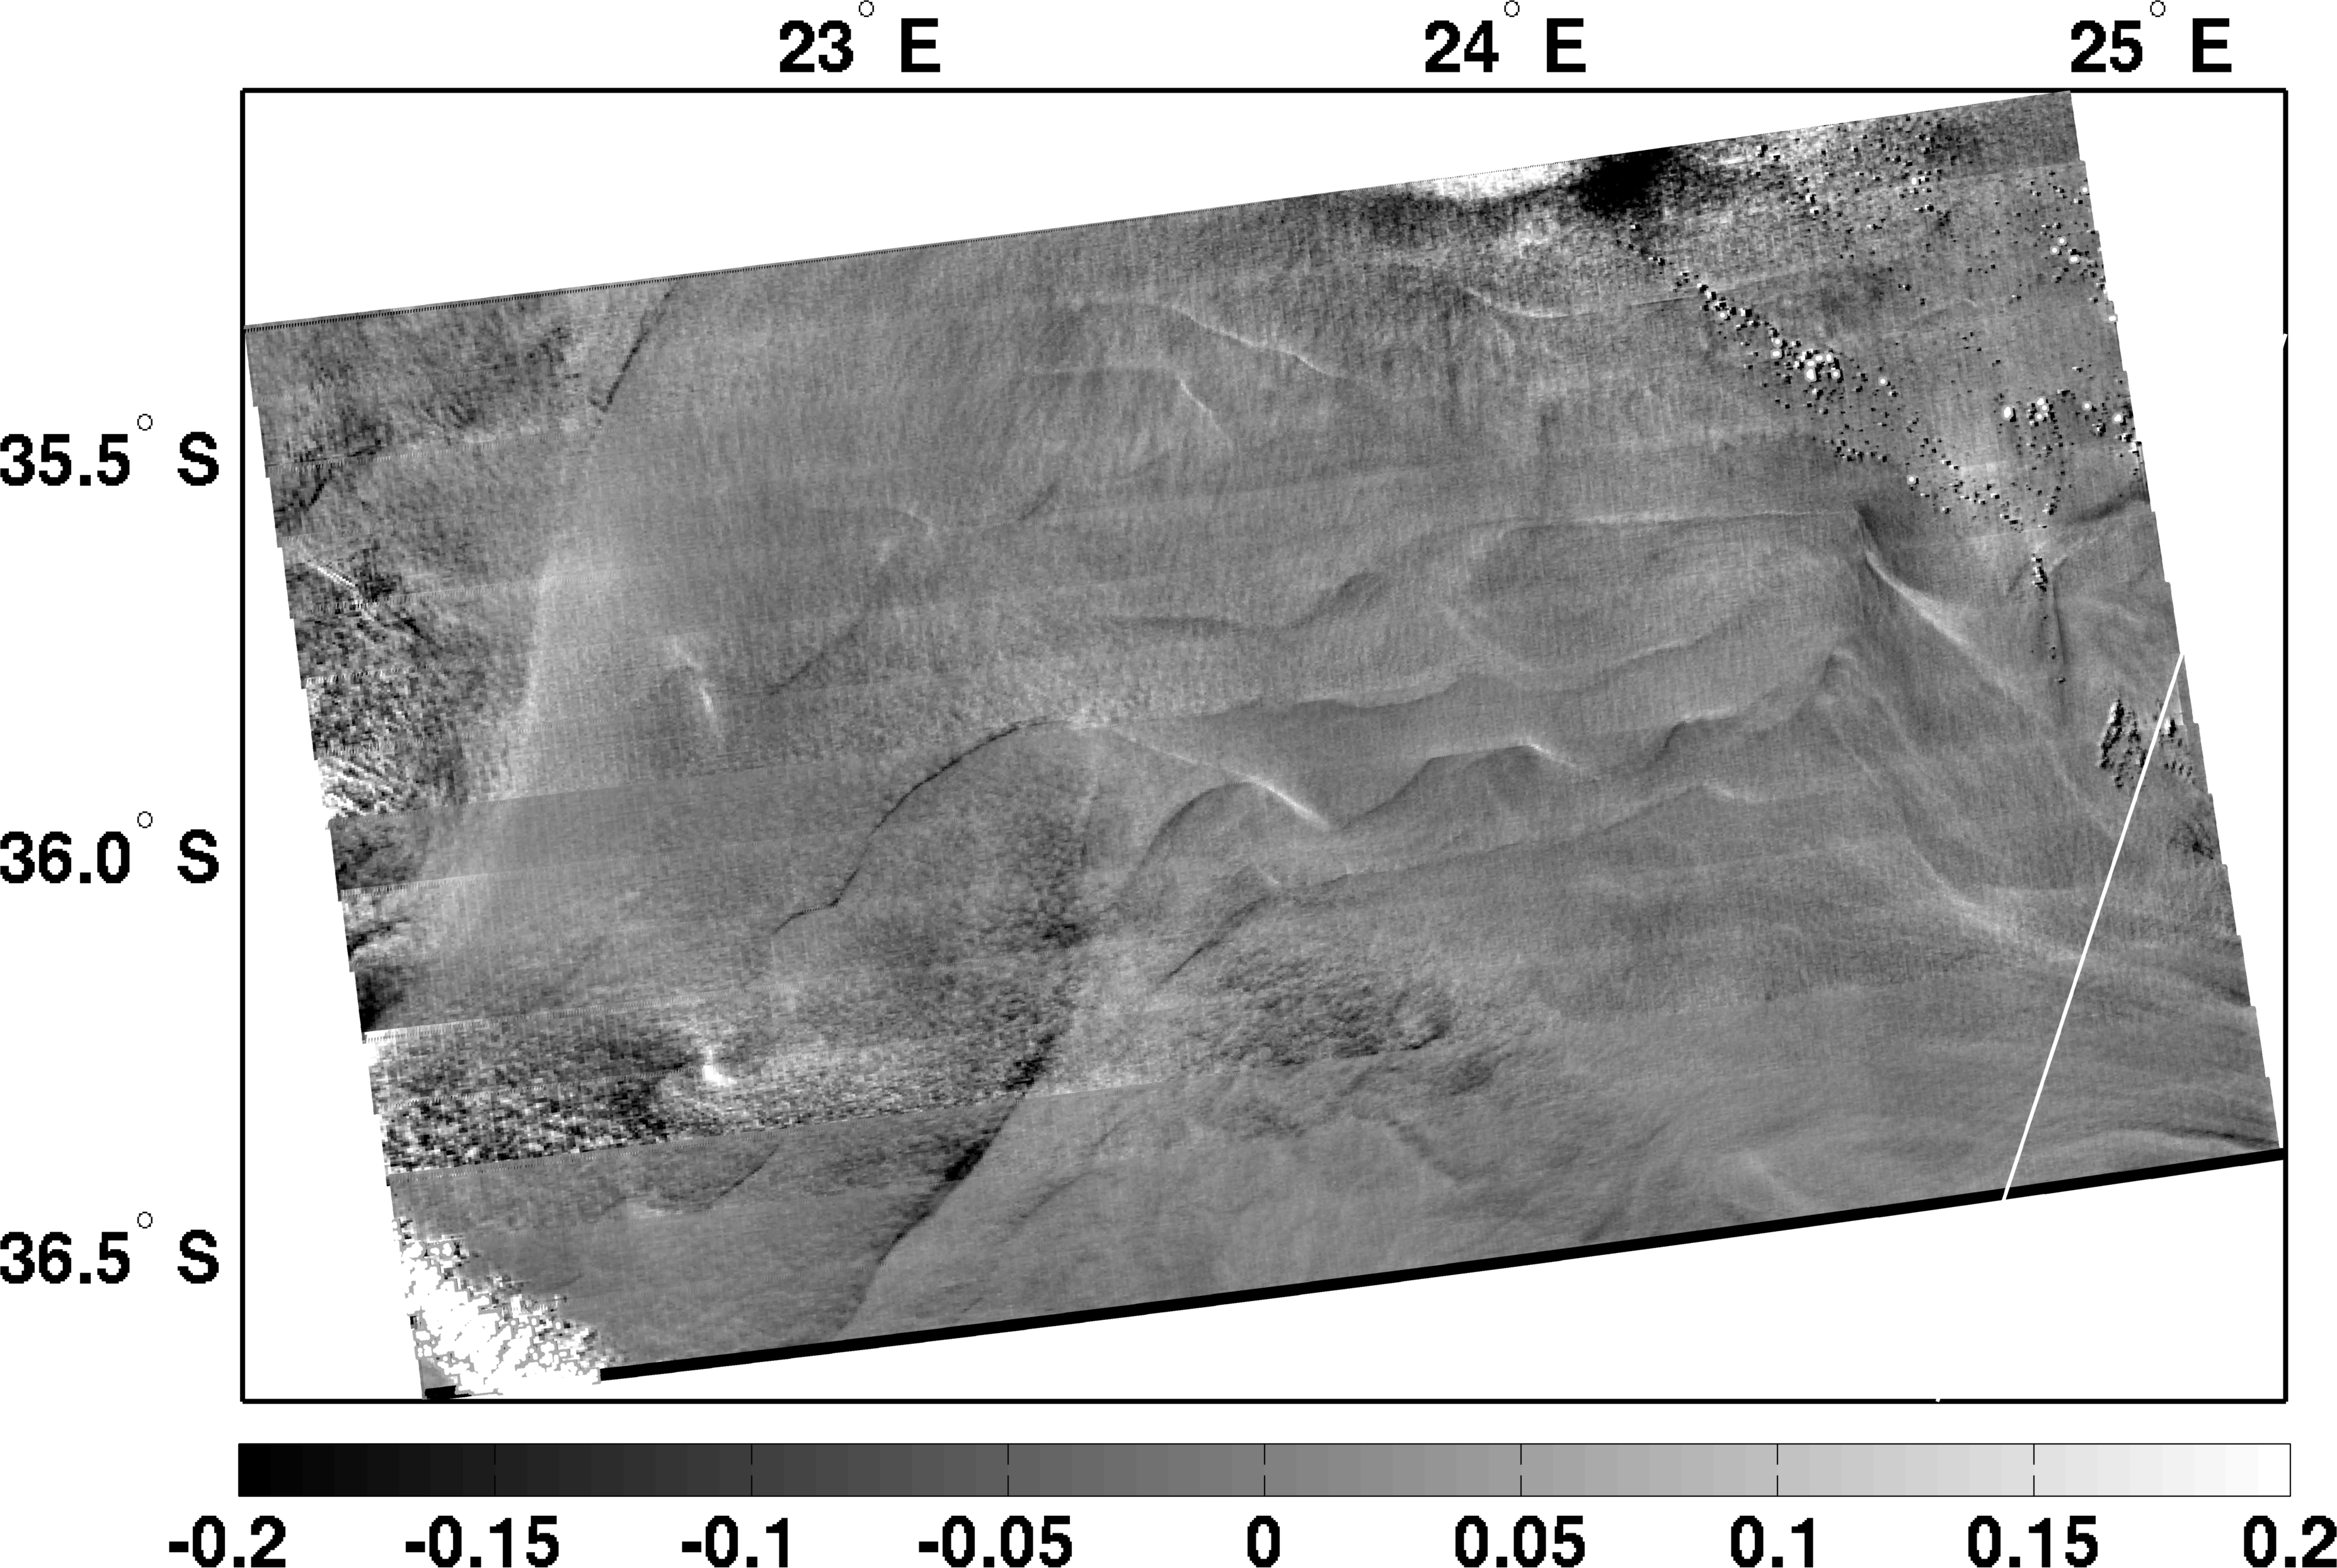
\includegraphics[width=1\linewidth]{fig3_8a}}
	\end{minipage}
	\hfill
	\begin{minipage}{.47\textwidth}
	    \subcaptionbox{\label{fig:3.8b}}
		{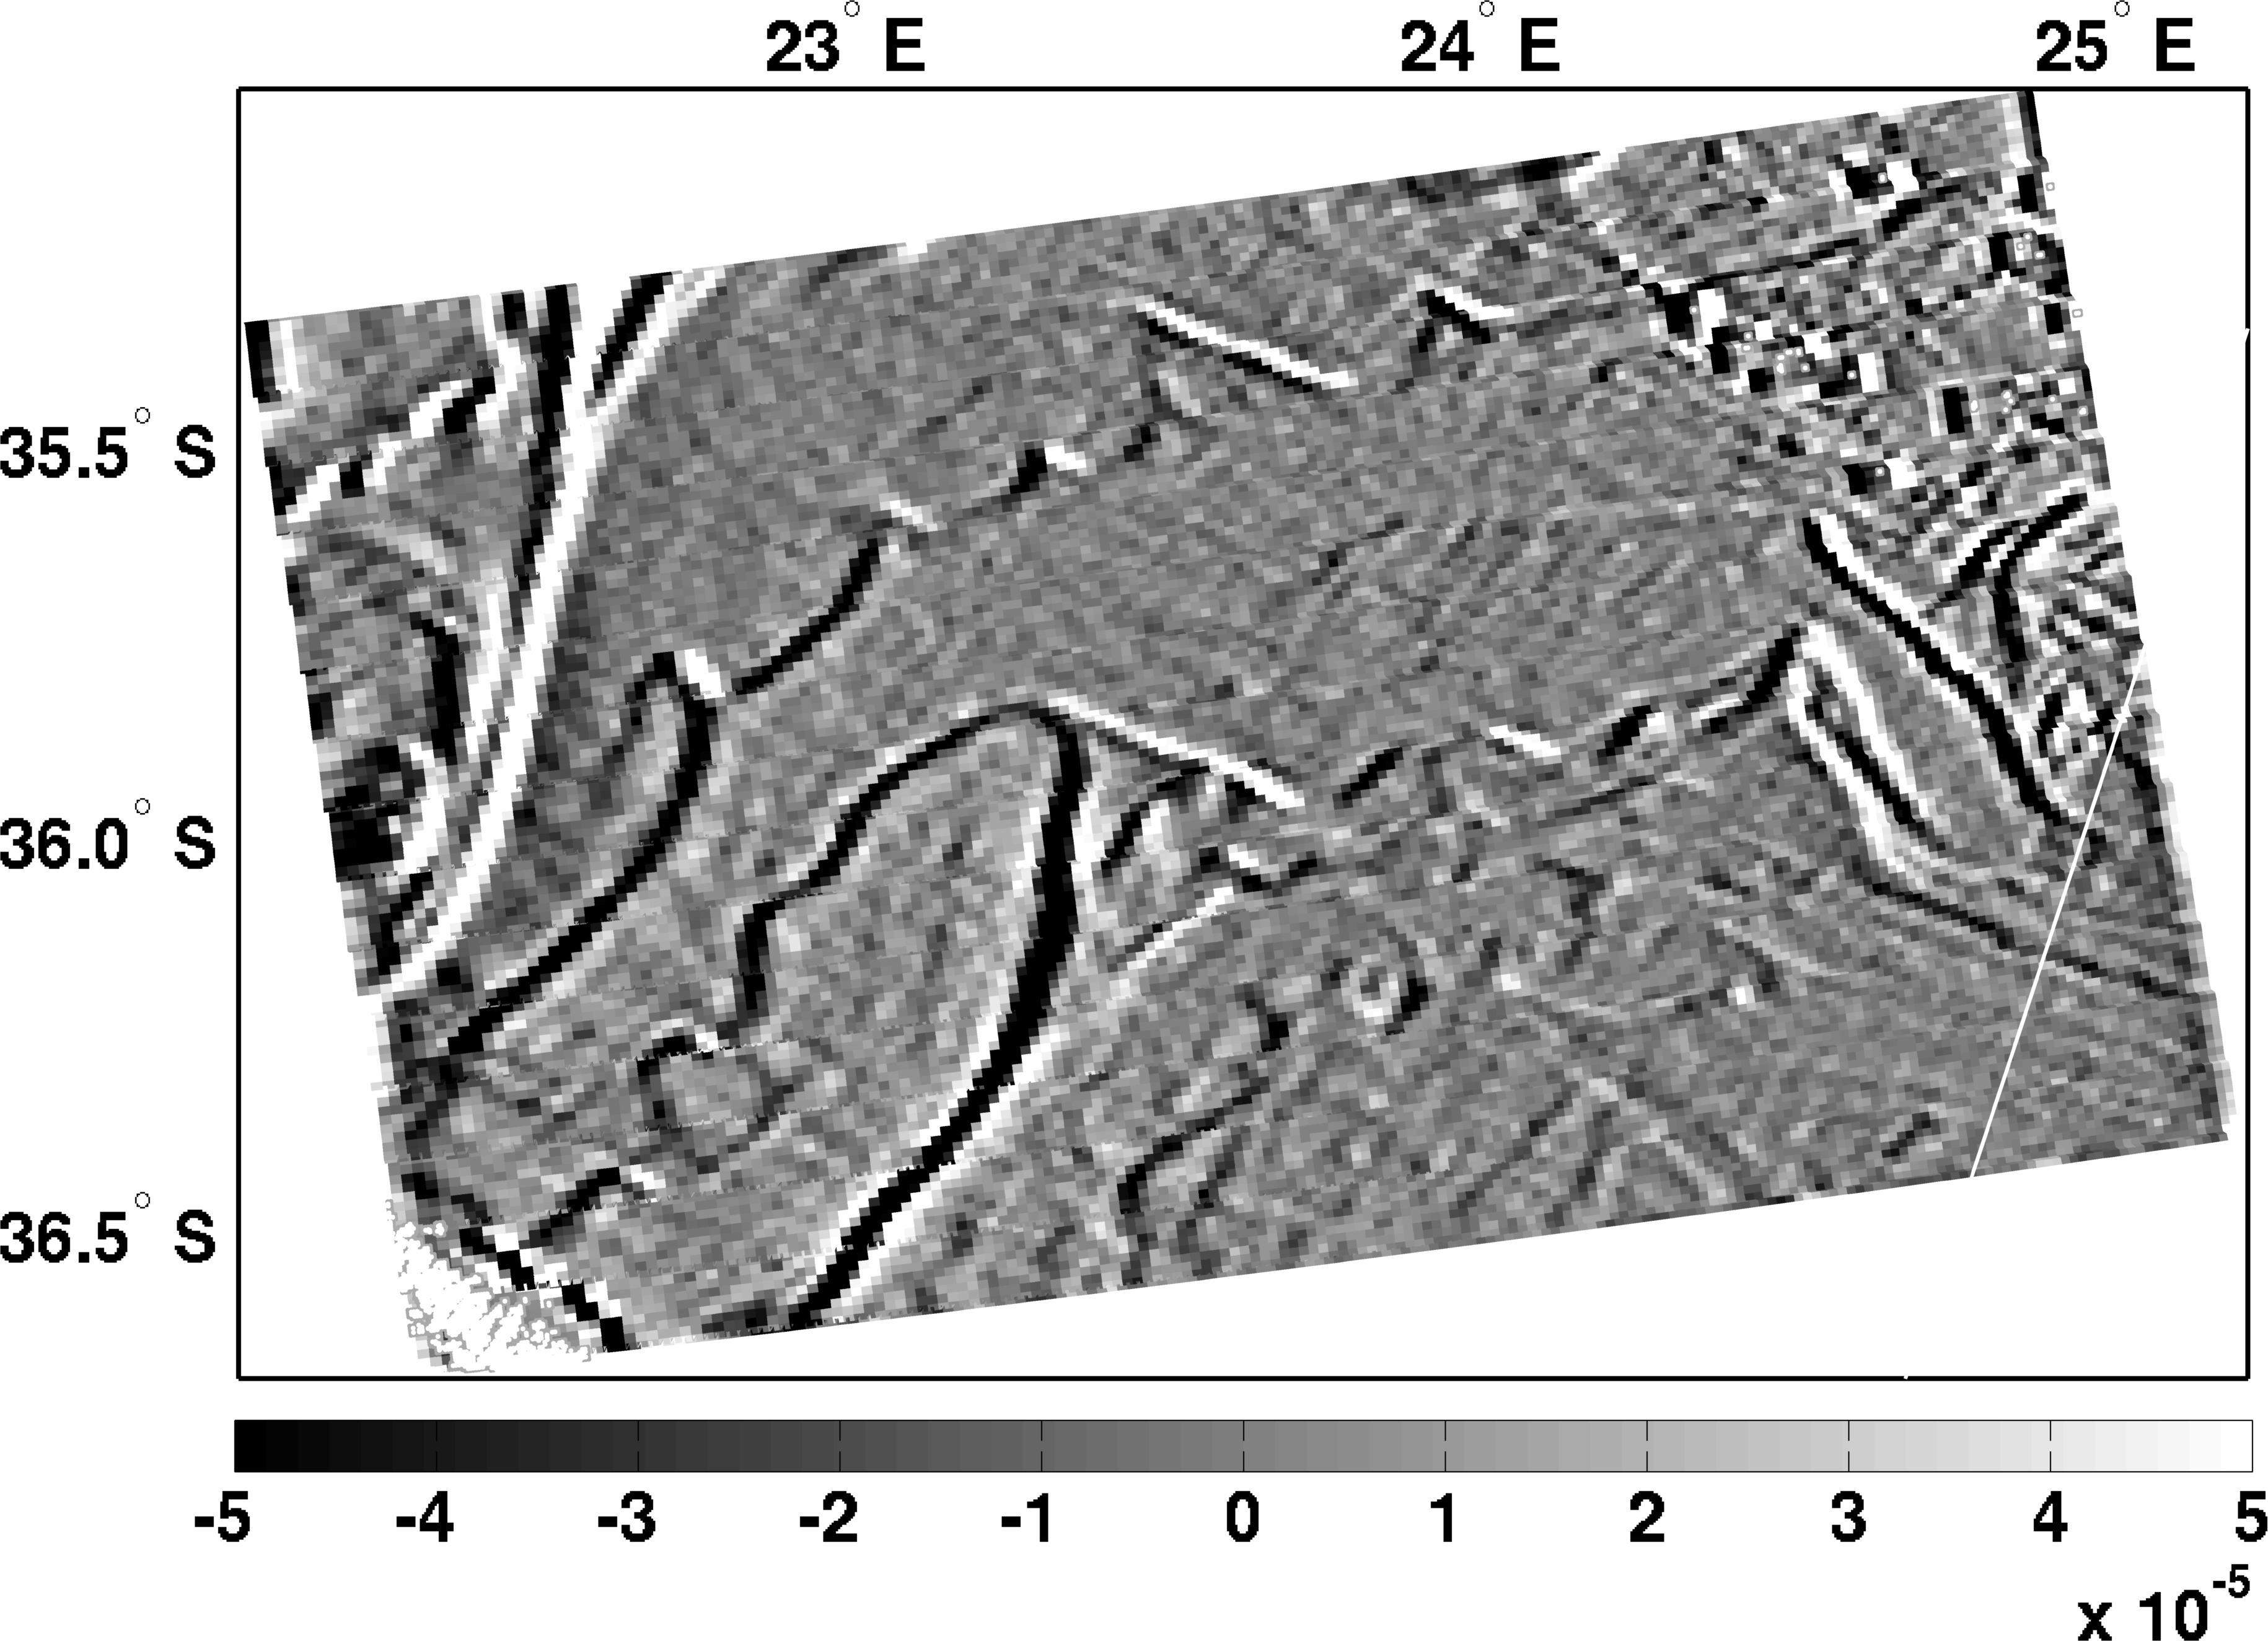
\includegraphics[width=1\linewidth]{fig3_8b}}
	\end{minipage}
    \\
    \floattitle{(а) Фрагмент поля контрастов СКН, показанный ранее на Рисунке~\ref{fig:3.5}. (б) Поле дивергенции поверхностного течения. Наблюдаемое различие между полями дивергенции поверхностного течения на Рисунке~\ref{fig:3.8b} и соответствующей областью на Рисунке~\ref{fig:3.6b}, объясняется тем, что $\nabla \cdot {\it u}$, показанная на данном рисунке, рассчитывалась для локального Северного ветра, в то время как $\nabla \cdot {\it u}$, показанная на Рисунке~\ref{fig:3.6b} в этом же районе, была рассчитана для Южного ветра (подробнее в тексте). Яркие области на рисунке (б) соответствуют конвергенции течения, а тёмные -- дивергенции (детальнее см. подпись к Рисунку~\ref{fig:3.6})}
    \caption{Фрагменты поля контрастов СКН и дивергенции поверхностного течения}
    \label{fig:3.8}
\end{figure}


На Рисунке~\ref{fig:3.9}, в поле ТПО (Рисунок~\ref{fig:3.9a}), а также в поле дивергенции поверхностного течения (Рисунок~\ref{fig:3.9b}), отчётливо видна пара вихрей, образующих грибовидную структуру. Вместе с соответствующими полем контрастов СКН (Рисунок~\ref{fig:3.9c}) и полем контрастов УЭПР РСА (Рисунок~\ref{fig:3.9d}), изображающими ту же пару вихрей, на рисунках видно поражающее сходство в геометрии поверхностных проявлений на всех четырёх изображениях, что ещё раз подчёркивает удивительные возможности совместного использования оптических и радиолокационных данных.



\begin{figure}[H]
   	\centering
	\begin{minipage}{.47\textwidth}
	    \subcaptionbox{\label{fig:3.9a}}
		{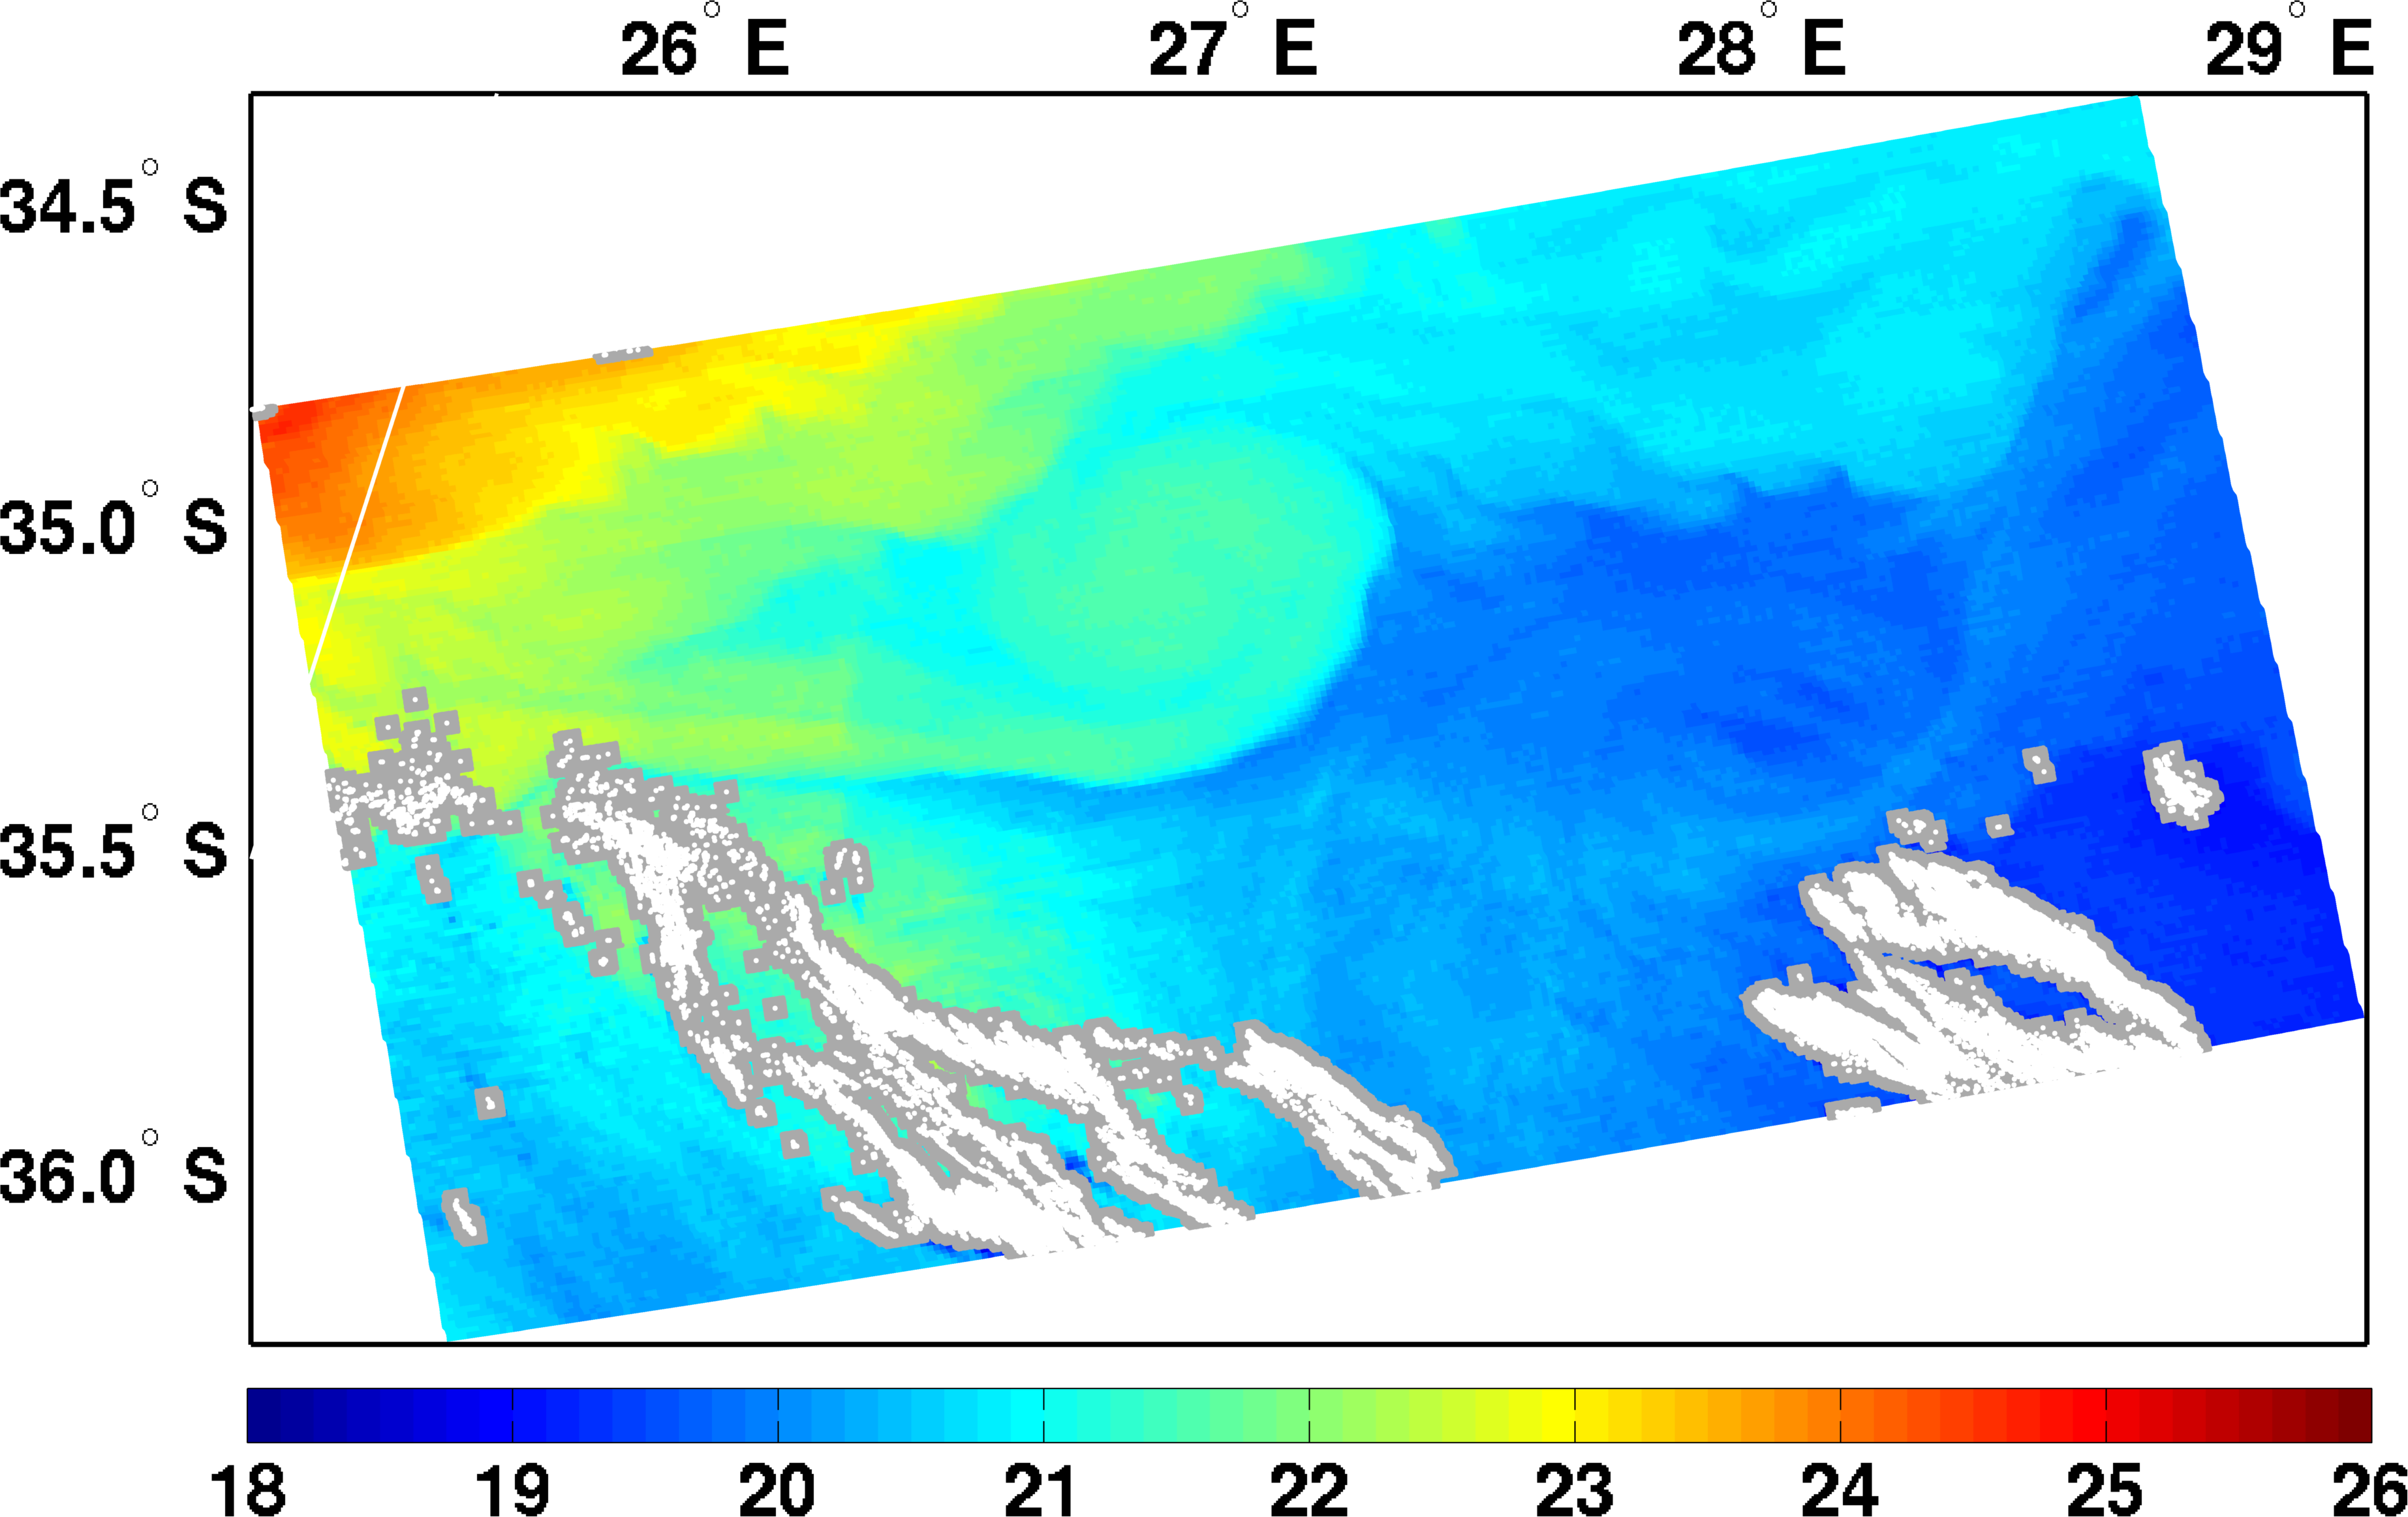
\includegraphics[width=1\linewidth]{fig3_9a}}
	\end{minipage}
	\hfill
	\begin{minipage}{.47\textwidth}
	    \subcaptionbox{\label{fig:3.9b}}
		{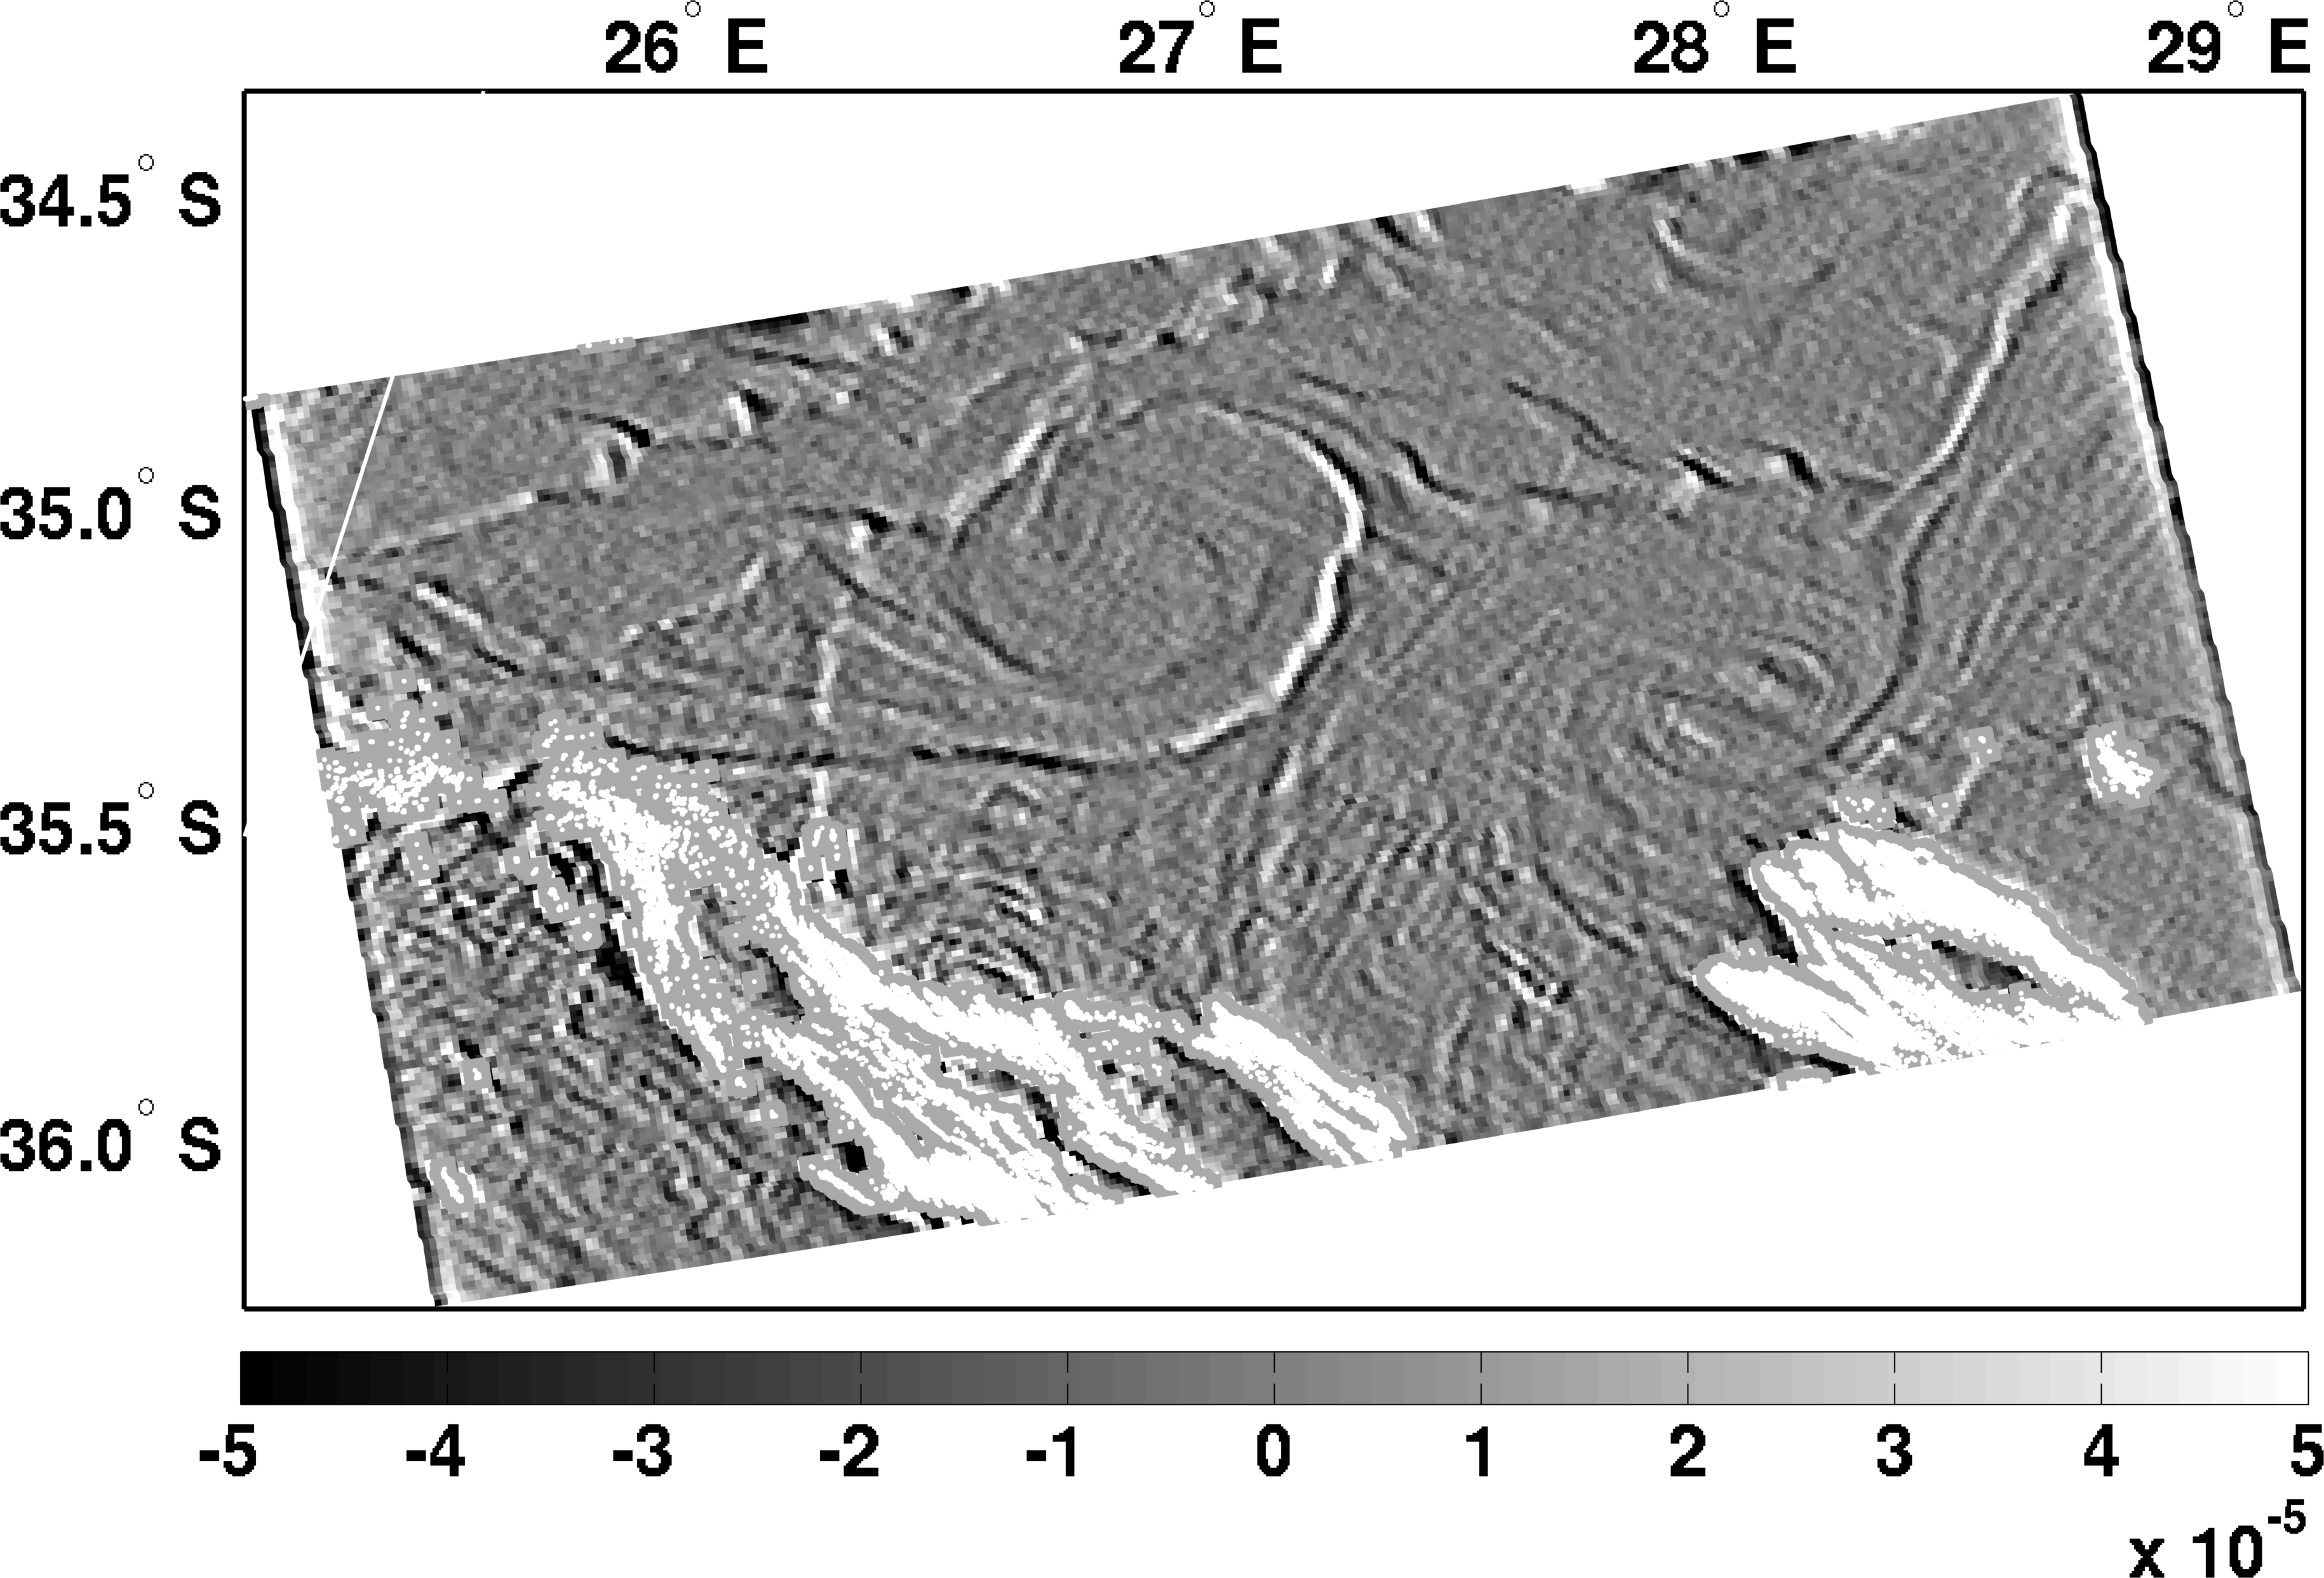
\includegraphics[width=1\linewidth]{fig3_9b}}
	\end{minipage}
	\\
	\begin{minipage}{.47\textwidth}
	    \subcaptionbox{\label{fig:3.9c}}
		{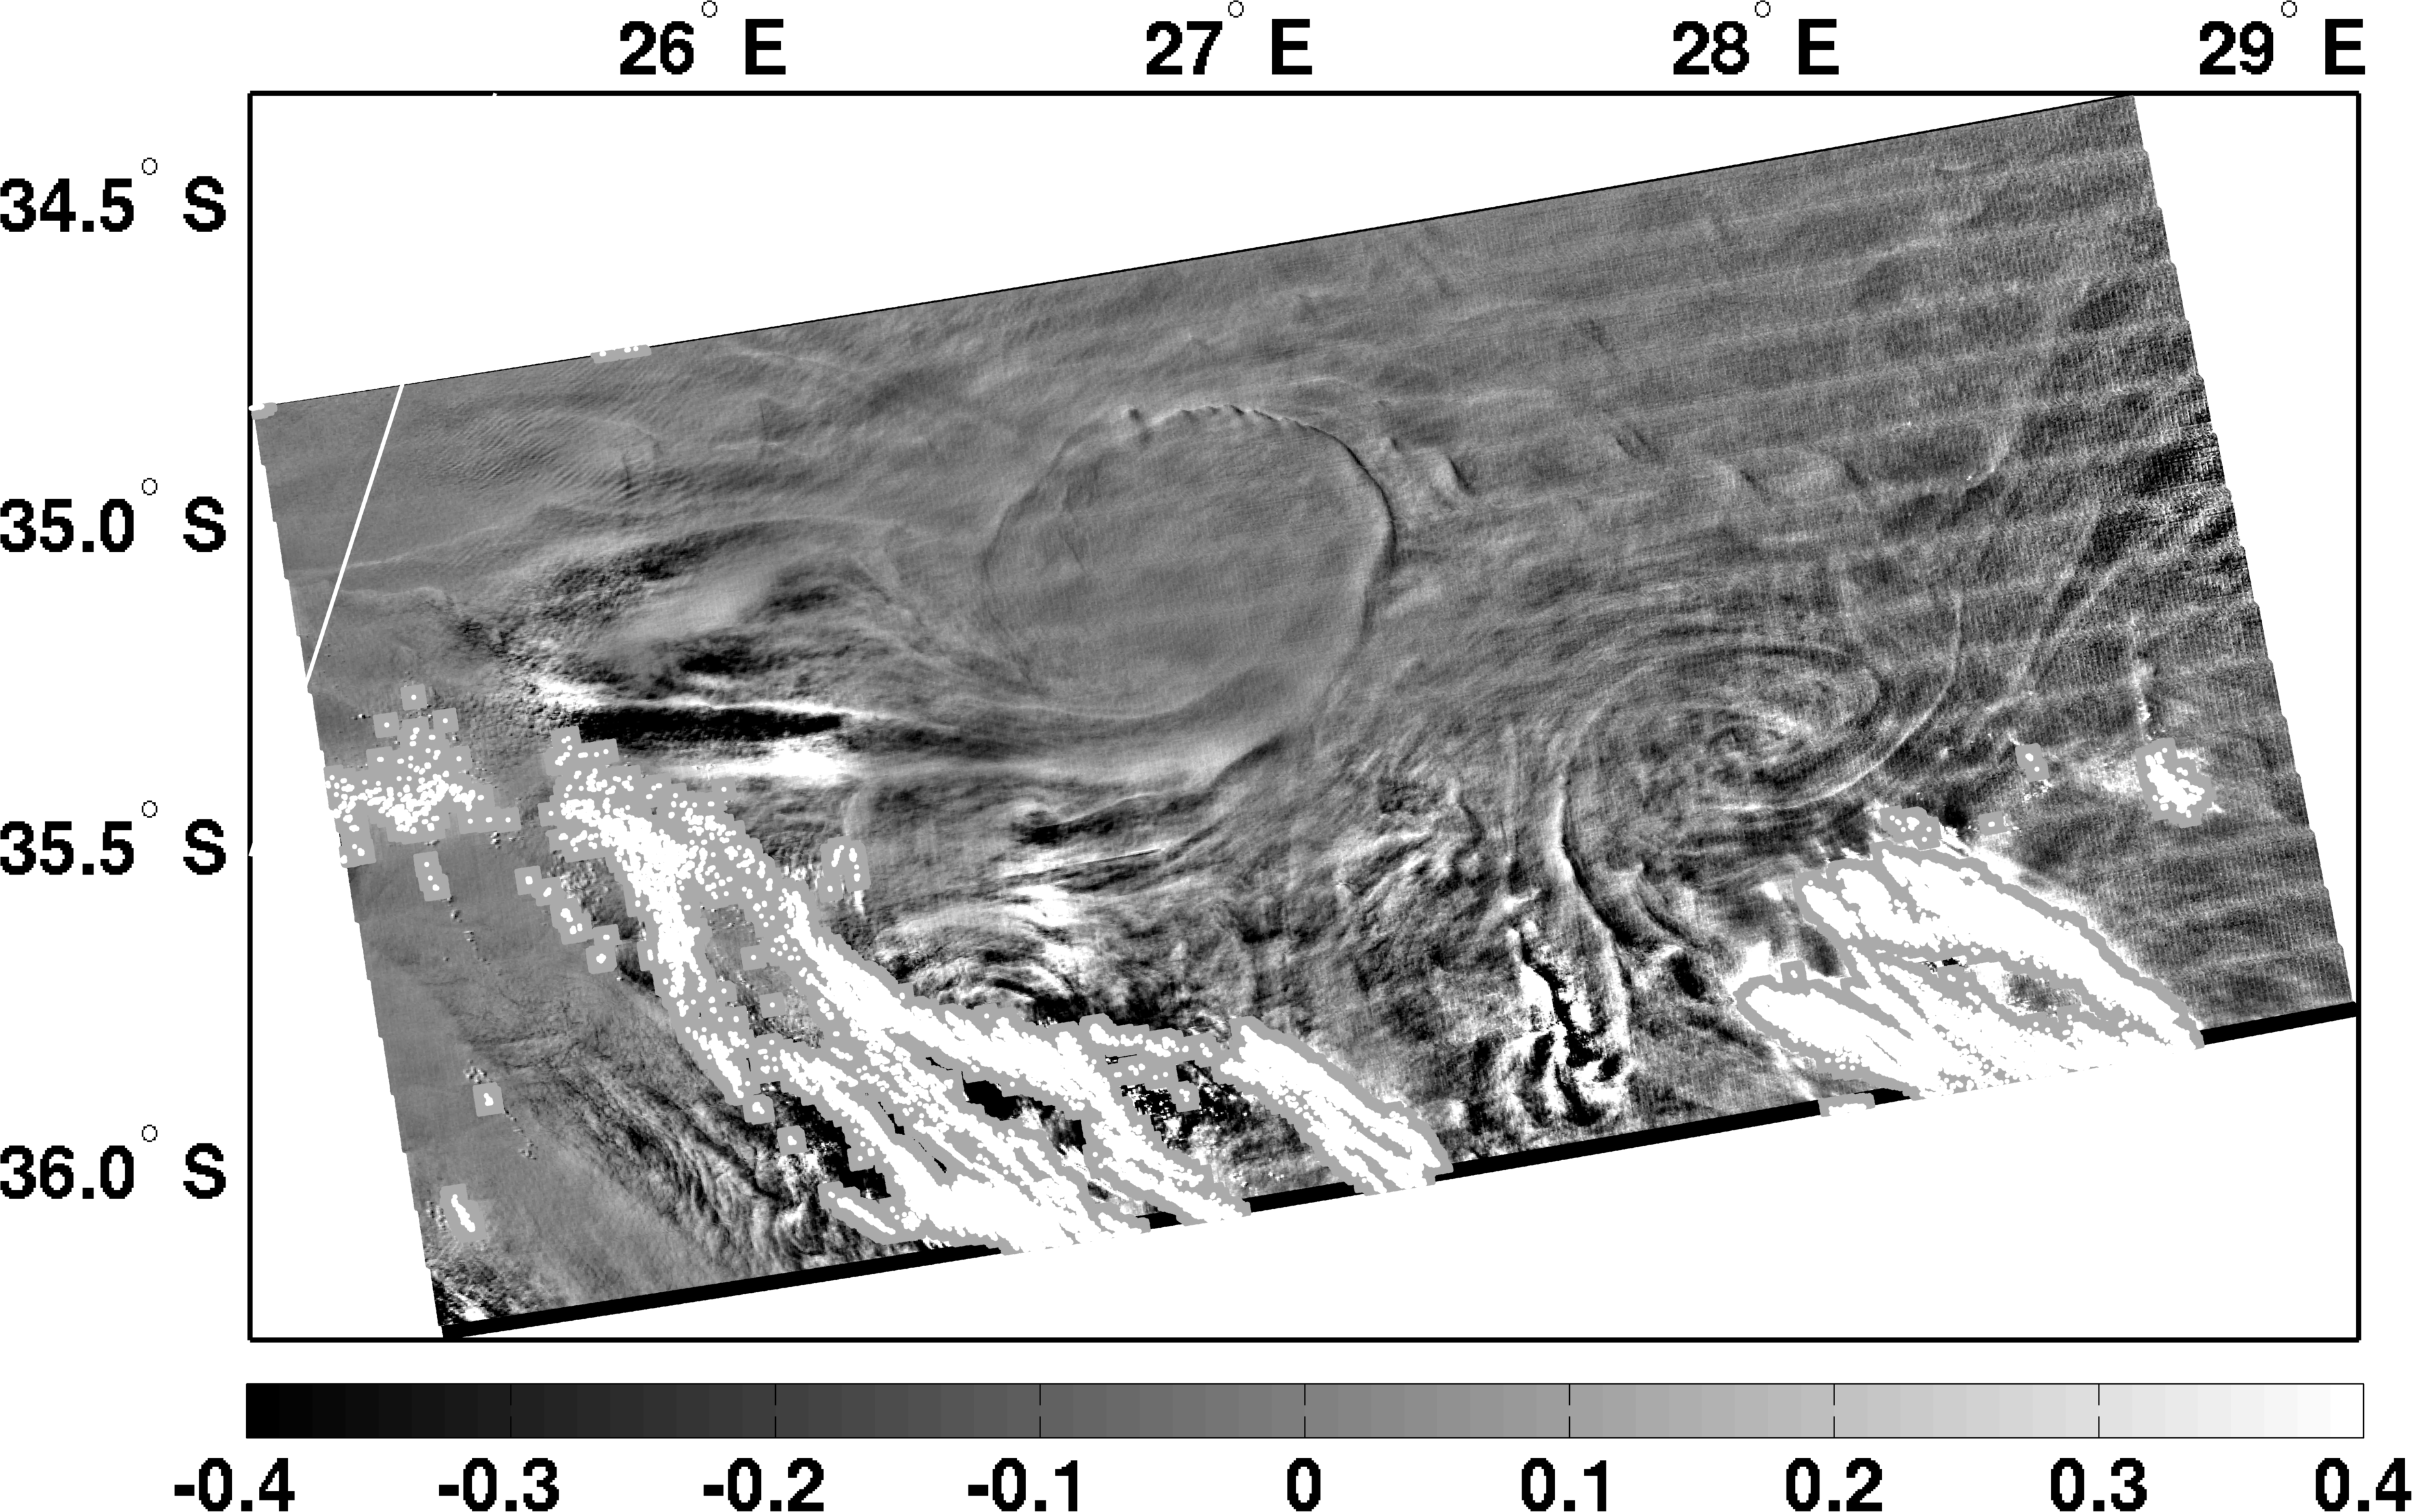
\includegraphics[width=1\linewidth]{fig3_9c}}
	\end{minipage}
	\hfill
	\begin{minipage}{.47\textwidth}
	    \subcaptionbox{\label{fig:3.9d}}
		{\includegraphics[width=1\linewidth]{fig3_9d}}
	\end{minipage}
    \\
    \floattitle{Поле ТПО MODIS (а), а также в поле дивергенции поверхностного течения (б), отчётливо видна пара вихрей диаметром 120км, образующих грибовидную структуру. Соответствующие поля СКН (в) и контрасты УЭПР РСА в линейных единицах (г), изображают ту же пару вихрей. Рисунки отражают поражающие возможности синергетического метода. Яркие области на рисунке (б) соответствуют конвергенции течения, а тёмные -- дивергенции (детальнее см. подпись к Рисунку~\ref{fig:3.6b})}
    \caption{Фрагменты поля контрастов СКН и дивергенции поверхностного течения}
    \label{fig:3.9}
\end{figure}



\section{Интерпретация данных наблюдений на основе модельных представлений} \label{sec:3.3}



\subsection{Результаты интерпретации данных} \label{sec:3.3.1}


Поле поверхностного течения, состоящее из суммы КГТ (см. Рисунок~\ref{fig:3.6a}), Экмановского дрейфа и ВАЦ и полученное по данным ТПО MODIS (см. Рисунок~\ref{fig:3.3b}) и полям ветра ENVISAT ASAR (см. Рисунок~\ref{fig:3.3a}), используется в качестве входных параметров модели формирования РЛ-изображения RIM, для моделирования РСА УЭПР и СКН сигнатур, как изложено в \citep{Kudryavtsev2005,Johannessen2005}, а также для расчёта трансформации эволюции спектров волн. Основные соотношения модели приведены в Приложении~\ref{AppendixA}.

На Рисунке~\ref{fig:3.10} приводятся сечения через контрасты спектра брэгговских волновых чисел, нормированных на фоновый спектр, рассчитанные по модели RIM. Видны различия контрастов спектра брэгговских волновых чисел, рассчитанных для сечения вдоль поля поверхностного течения, приведённого на Рисунке~\ref{fig:3.6}, при различных направлениях ветра. Из Рисунка~\ref{fig:3.10} видно, что для бокового ветра вариации контрастов значительно выше, а для направлений против и по ветру -- они минимальны.



\begin{figure}[H]
    
\includegraphics[width=\linewidth]{fig3_10}
    \floattitle{(слева) Сечение через контрасты спектра брэгговских волновых чисел, нормированных на фоновый спектр, рассчитанные по модели RIM для бокового ветра (сплошная синяя линия) и направления визирования против ветра (красная линия с крестиками). (справа) Контрасты спектра брэгговских волновых чисел для различных направлений ветра. Отчётливо видно, что для бокового ветра вариации контрастов значительно выше, а для направлений против и по ветру -- они минимальны}
    \caption{Различия контрастов спектра брэгговских волновых чисел, рассчитанных для сечения вдоль поля поверхностного течения, приведённого на Рисунке~\ref{fig:3.6}, при различных направлениях ветра }
    \label{fig:3.10}
\end{figure}


Смоделированные поверхностные проявления грибовидного вихря в терминах СКН, обрушений волн и контрастов УЭПР приводятся на Рисунке~\ref{fig:3.11} для угла падения 30${}^\circ$ и угла между вектором скорости ветра и направлением дальности 20${}^\circ$. Как и ожидалось, визуально геометрия этих двумерных полей очень схожи со структурой поля конвергенции поверхностного течения. Если присмотреться, можно заметить, что увеличение контрастов всех трёх приведённых полей происходит в области конвергенции течения (яркие области в верхнем левом углу изображения), в то время, как подавление возникает в зонах дивергенции (тёмные области). Этот результат численного моделирования соответствует упрощённому решению, определяемому уравнениями \eqref{eq:1.5}, \eqref{eq:1.7}, \eqref{eq:1.8} и \eqref{eq:1.9}. Стоит напомнить, что проявления особенностей мезомасштабных течений в УЭПР возникает в результате обрушений волн, обеспечивающих усиление/ослабление механических возмущений на поверхности в областях конвергенции/дивергенции. Это приводит к усилению/подавлению волн Брэгга и, тем самым, модуляции обратного рассеяния РЛ-сигнала.

Сравнивая симулированные поля контрастов УЭПР и СКН с наблюдаемыми на Рисунке~\ref{fig:3.9}, можно заметить, что модельные контрасты согласуются с наблюдаемыми значениями. Поскольку RIM была тщательно протестирована на имеющихся данных (см. \citep{Kudryavtsev2005}), этот факт предполагает, что восстановленные поля дивергенции поверхностного течения могут рассматриваться как близкие к ``реальным''. Также стоит отметить, что моделирование контрастов УЭПР для той же пары вихрей, без учёта влияния обрушений волн на УЭПР и модуляцию Брэгговских волн (``стандартная'' релаксационная модель) даёт контрасты УЭПР по величине на 4 порядка меньше, нежели приведённые на Рисунке~\ref{fig:3.11}.

Примеры результата расчётов СКН и обрушений волн с использованием уравнений \eqref{A.16} и \eqref{A.17} по модели RIM приводятся на Рисунке~\ref{fig:3.11}.

\begin{figure}[H]
   	\centering
	\begin{minipage}{.47\textwidth}
	    \subcaptionbox{\label{fig:3.11a}}
		{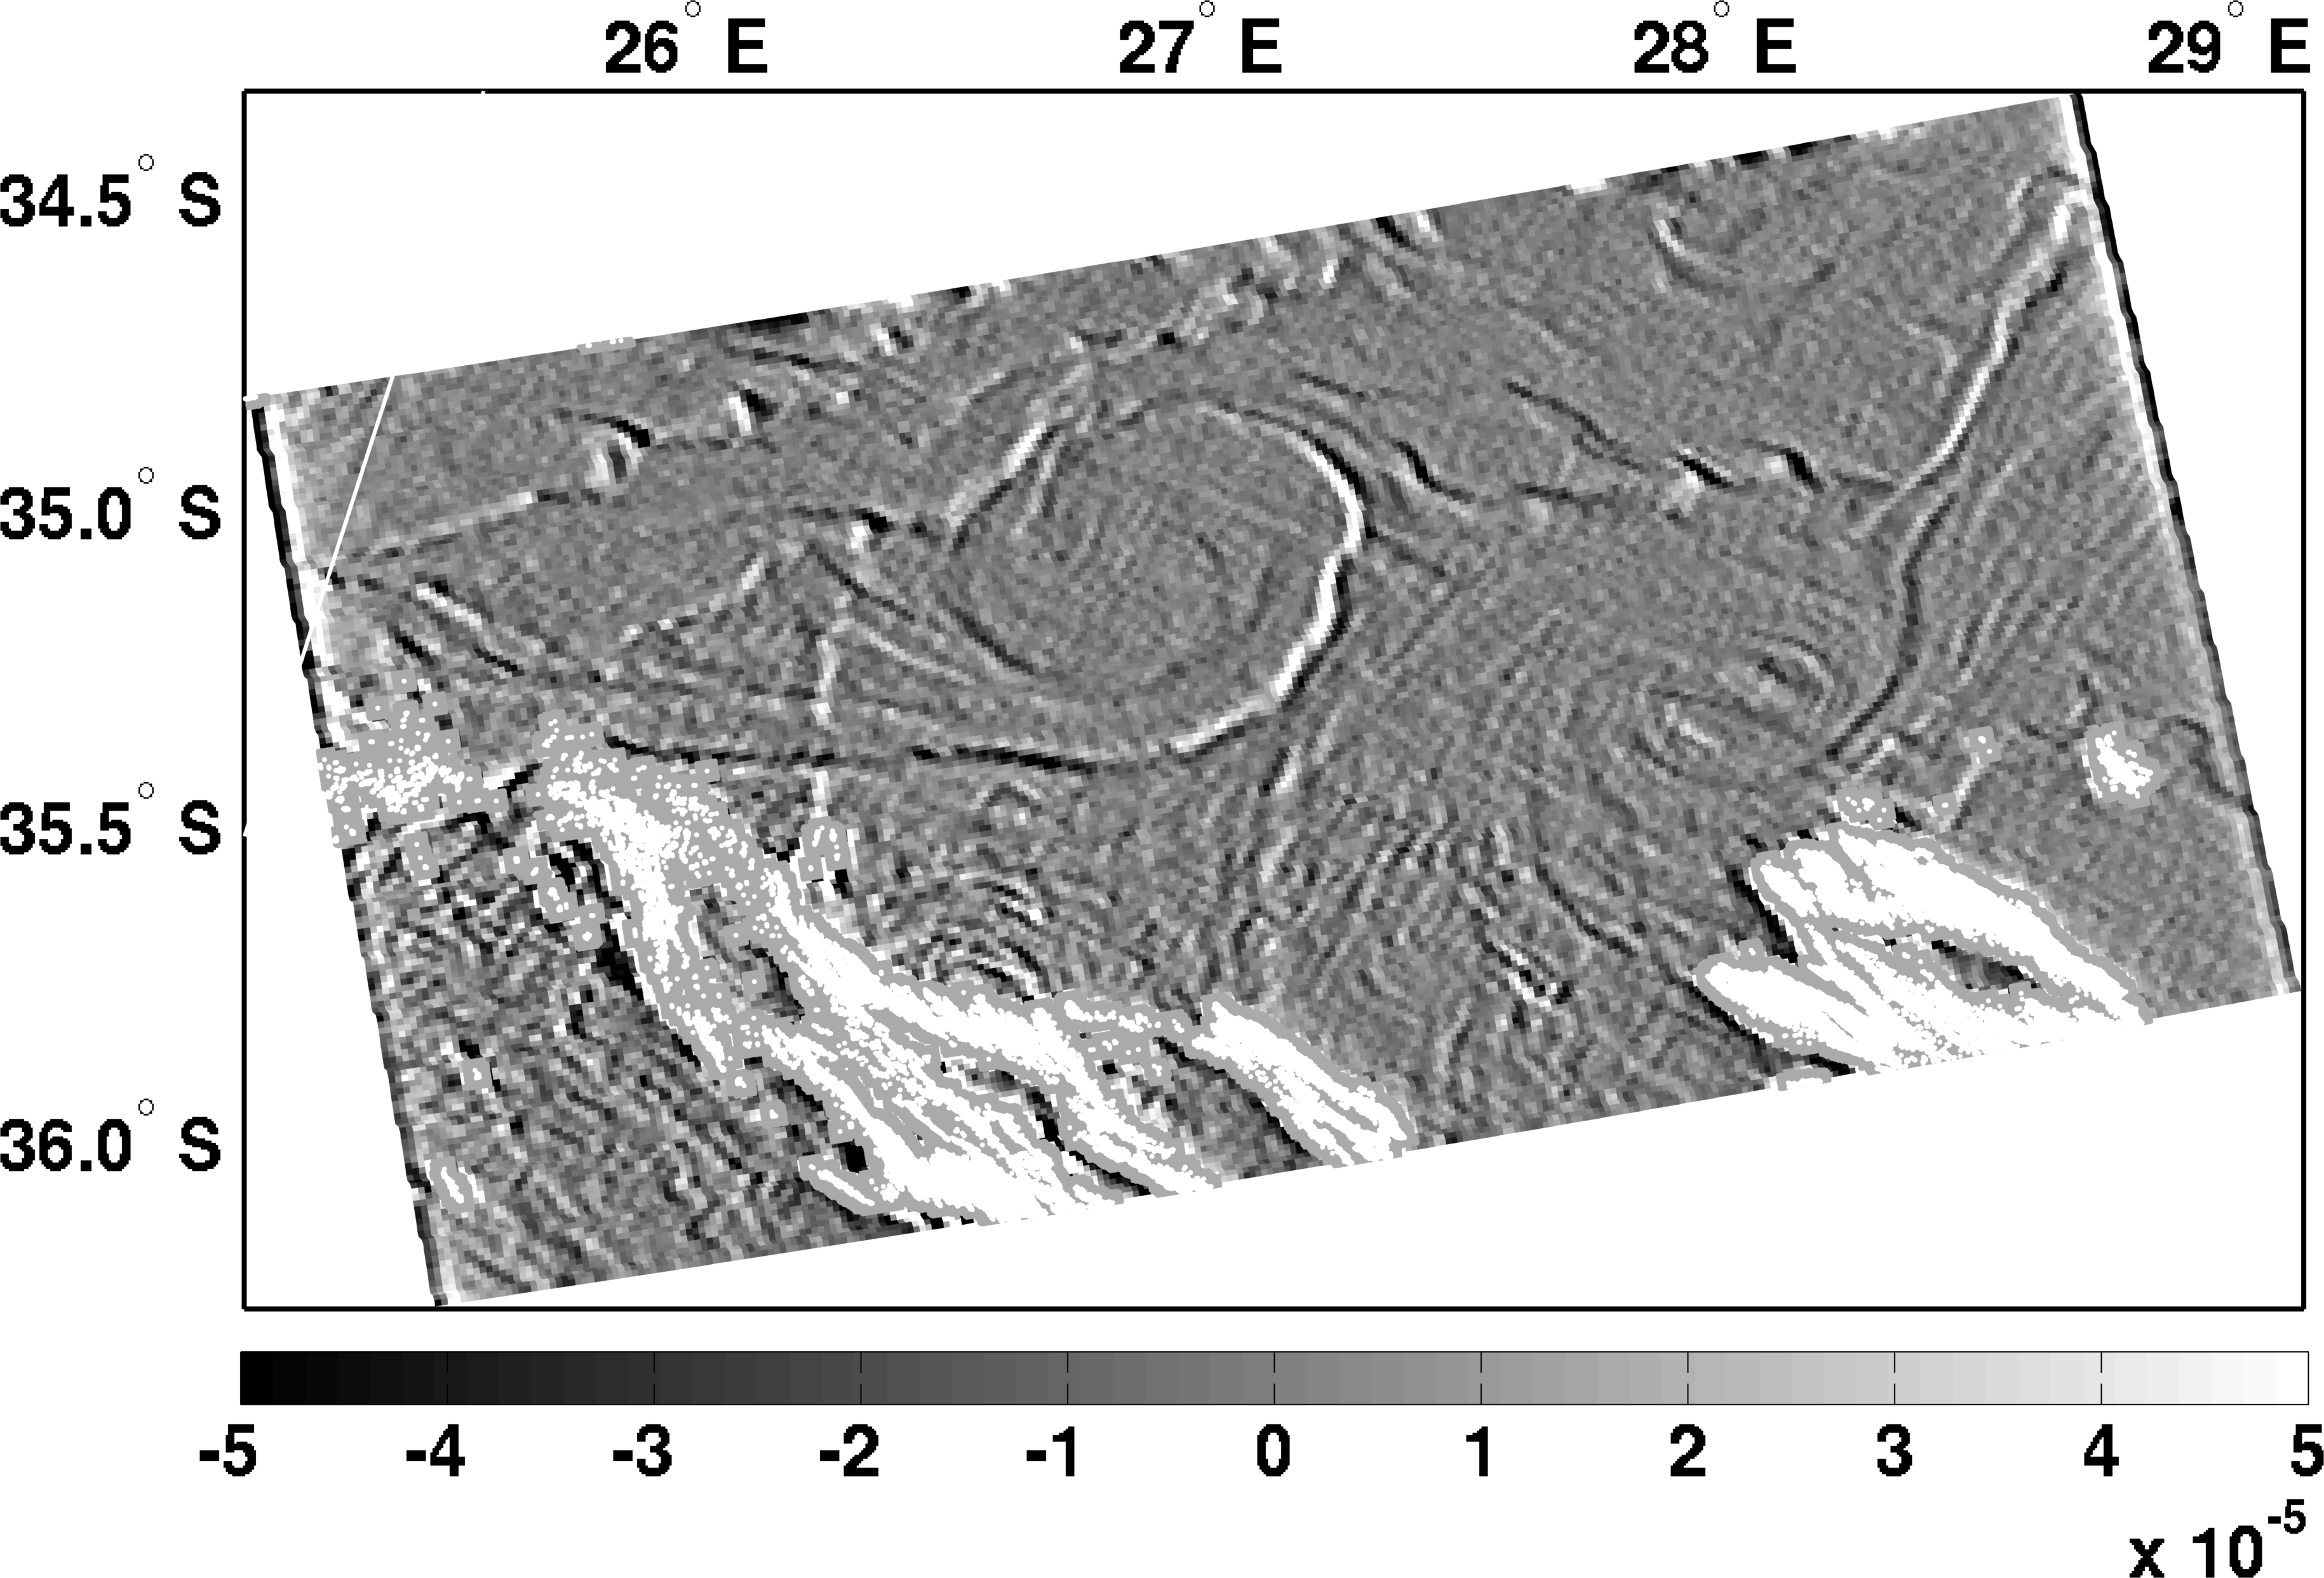
\includegraphics[width=1\linewidth]{fig3_11a}}
	\end{minipage}
	\hfill
	\begin{minipage}{.47\textwidth}
	    \subcaptionbox{\label{fig:3.11b}}
		{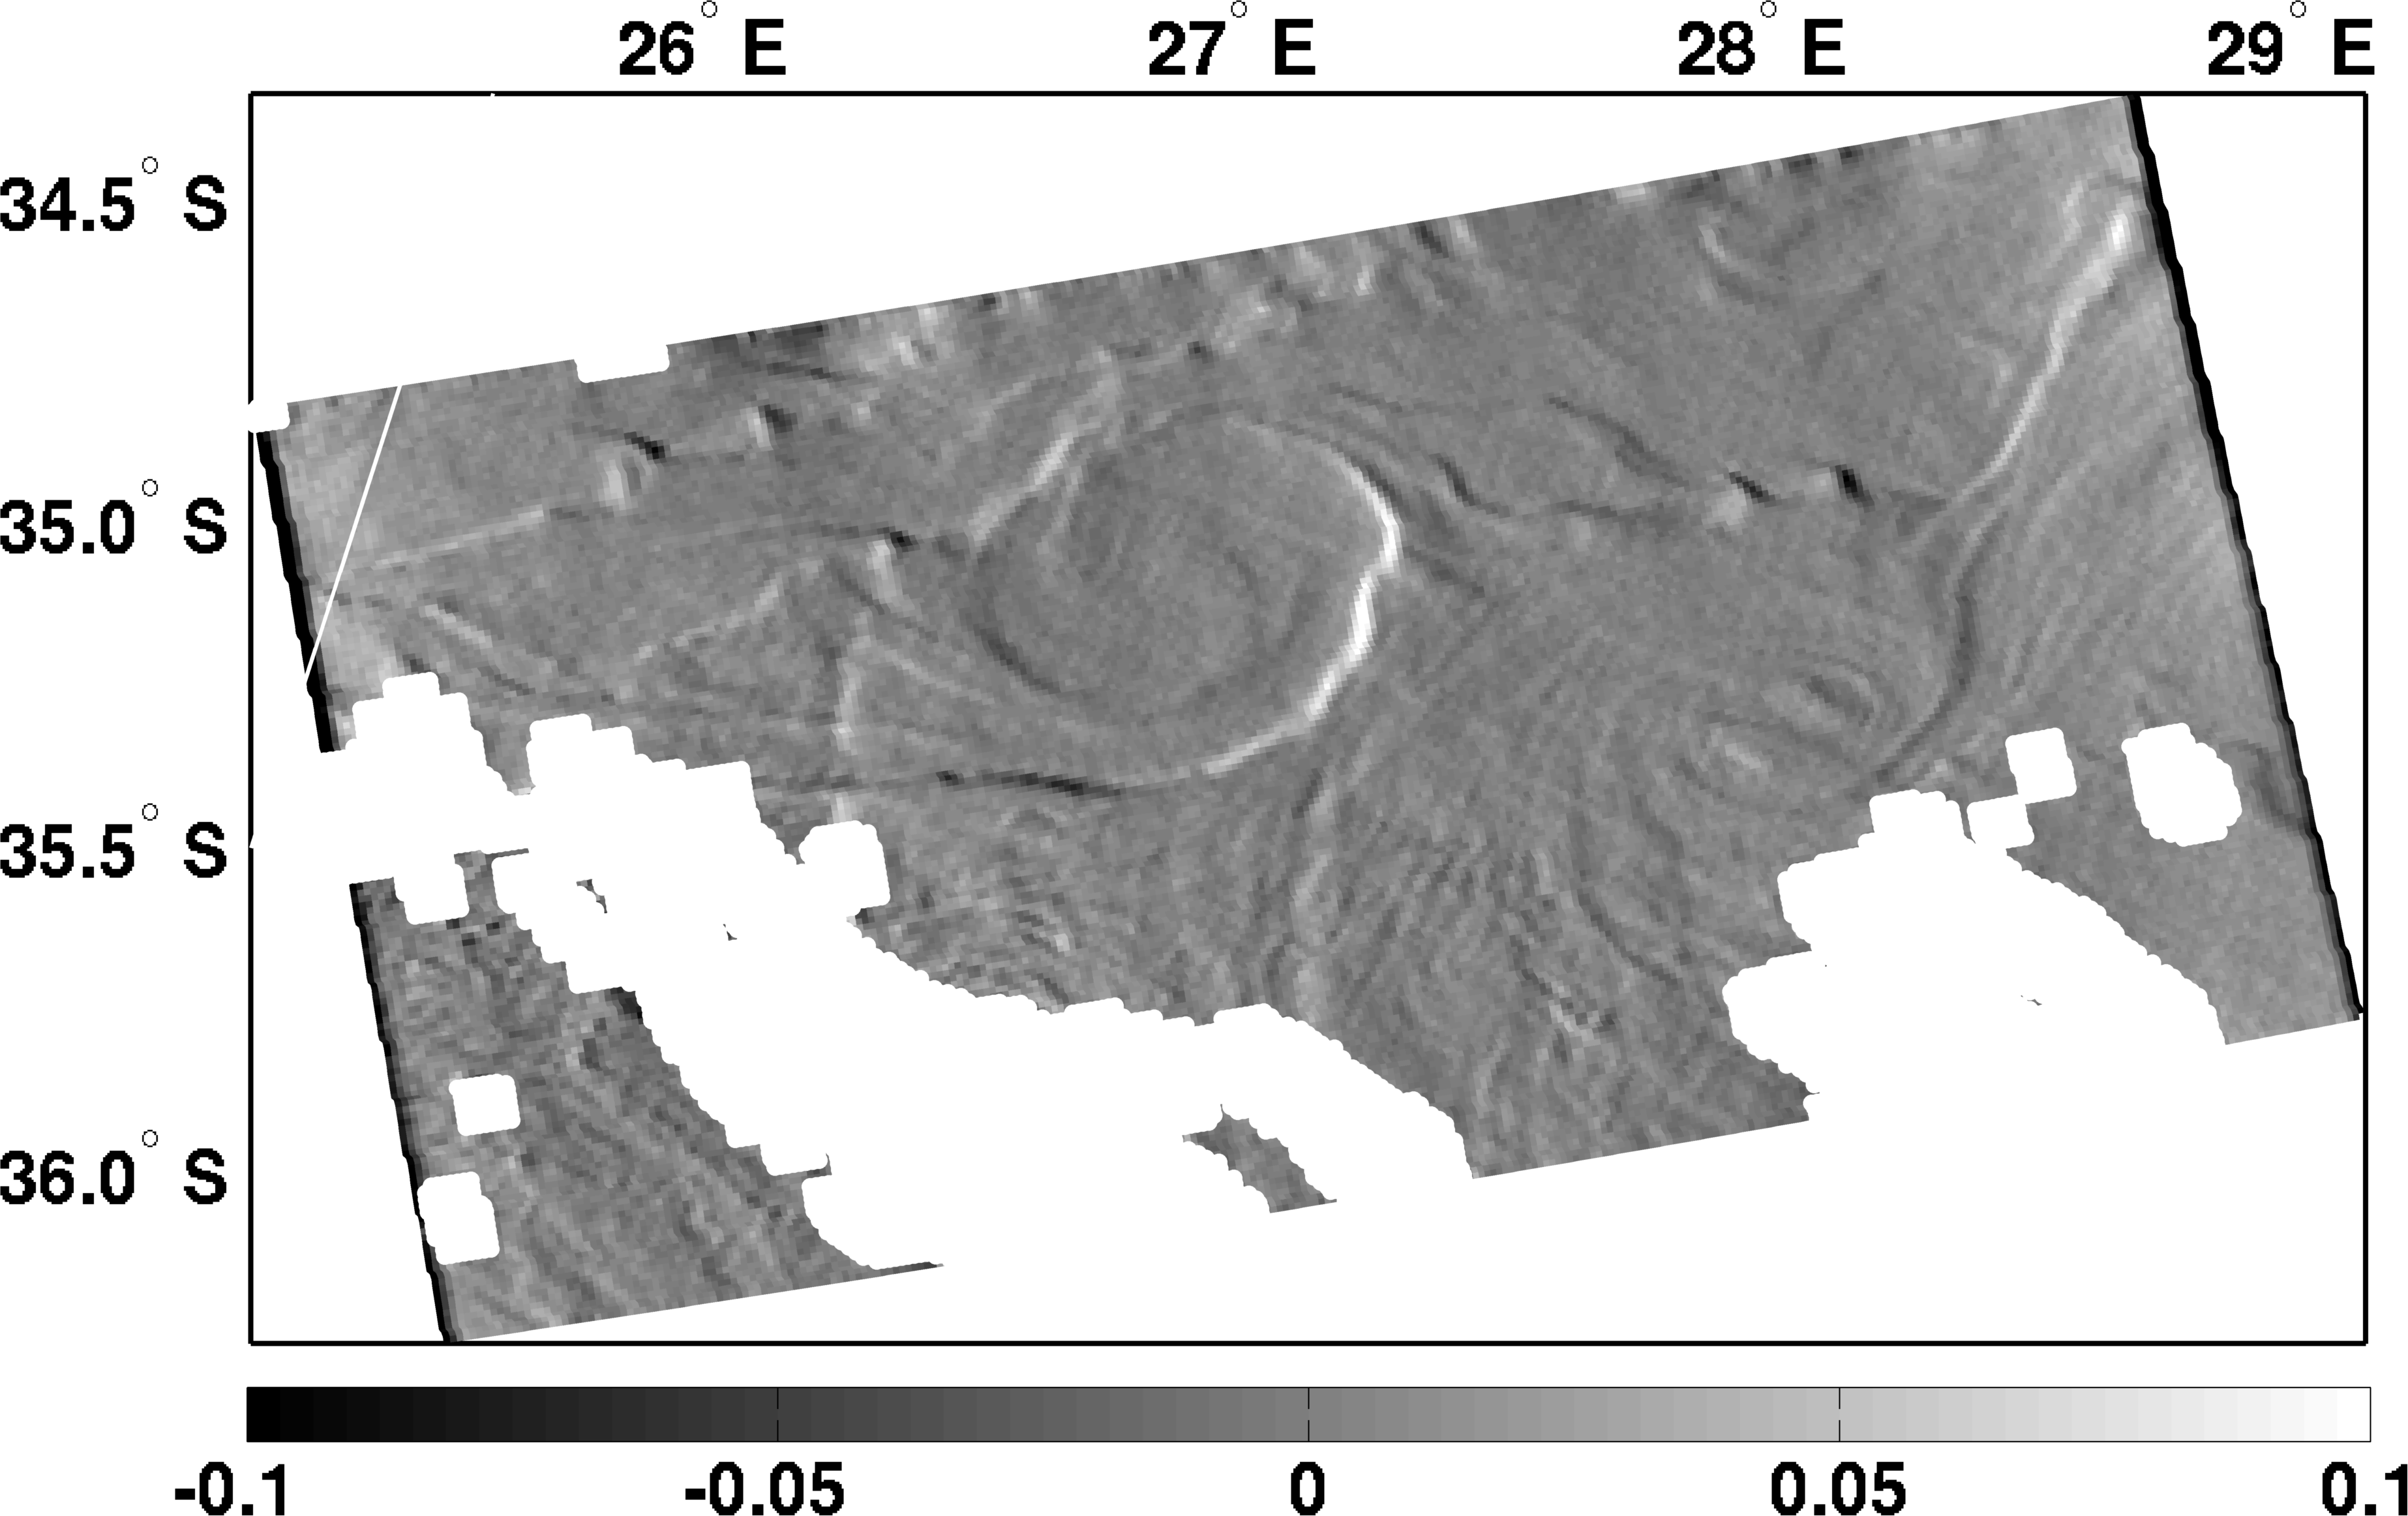
\includegraphics[width=1\linewidth]{fig3_11b}}
	\end{minipage}
	\\
	\begin{minipage}{.47\textwidth}
	    \subcaptionbox{\label{fig:3.11c}}
		{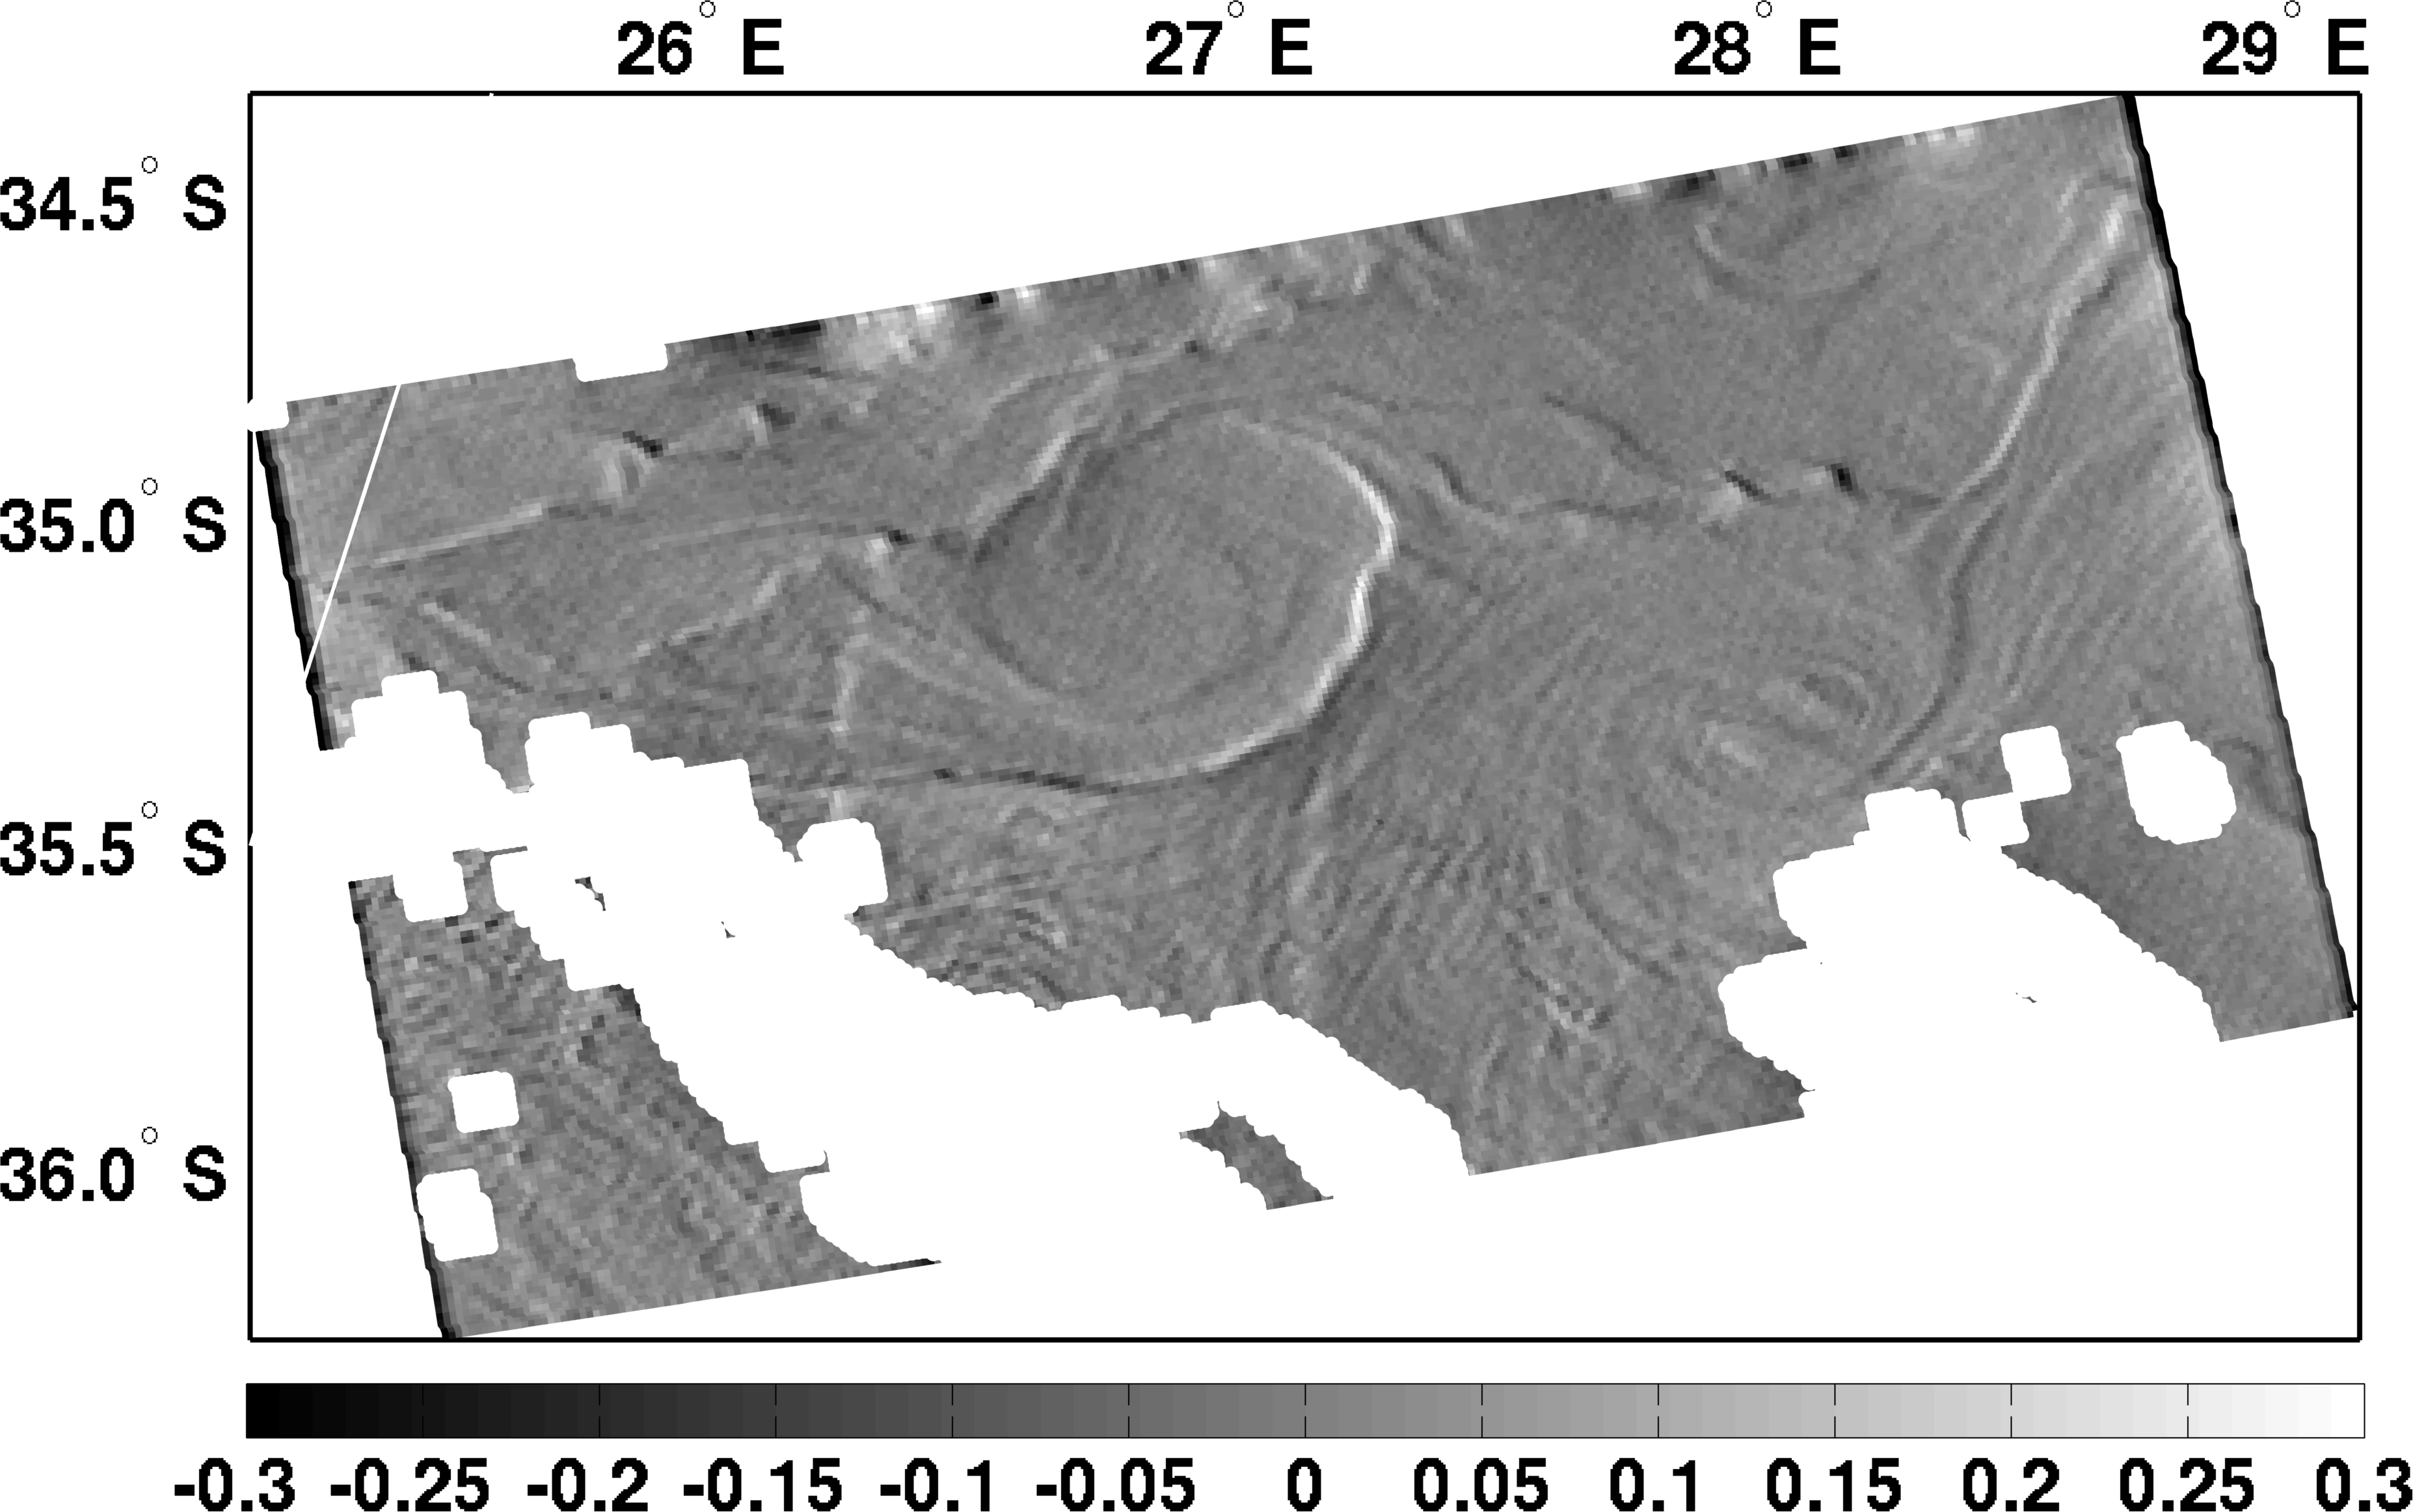
\includegraphics[width=1\linewidth]{fig3_11c}}
	\end{minipage}
	\hfill
	\begin{minipage}{.47\textwidth}
	    \subcaptionbox{\label{fig:3.11d}}
		{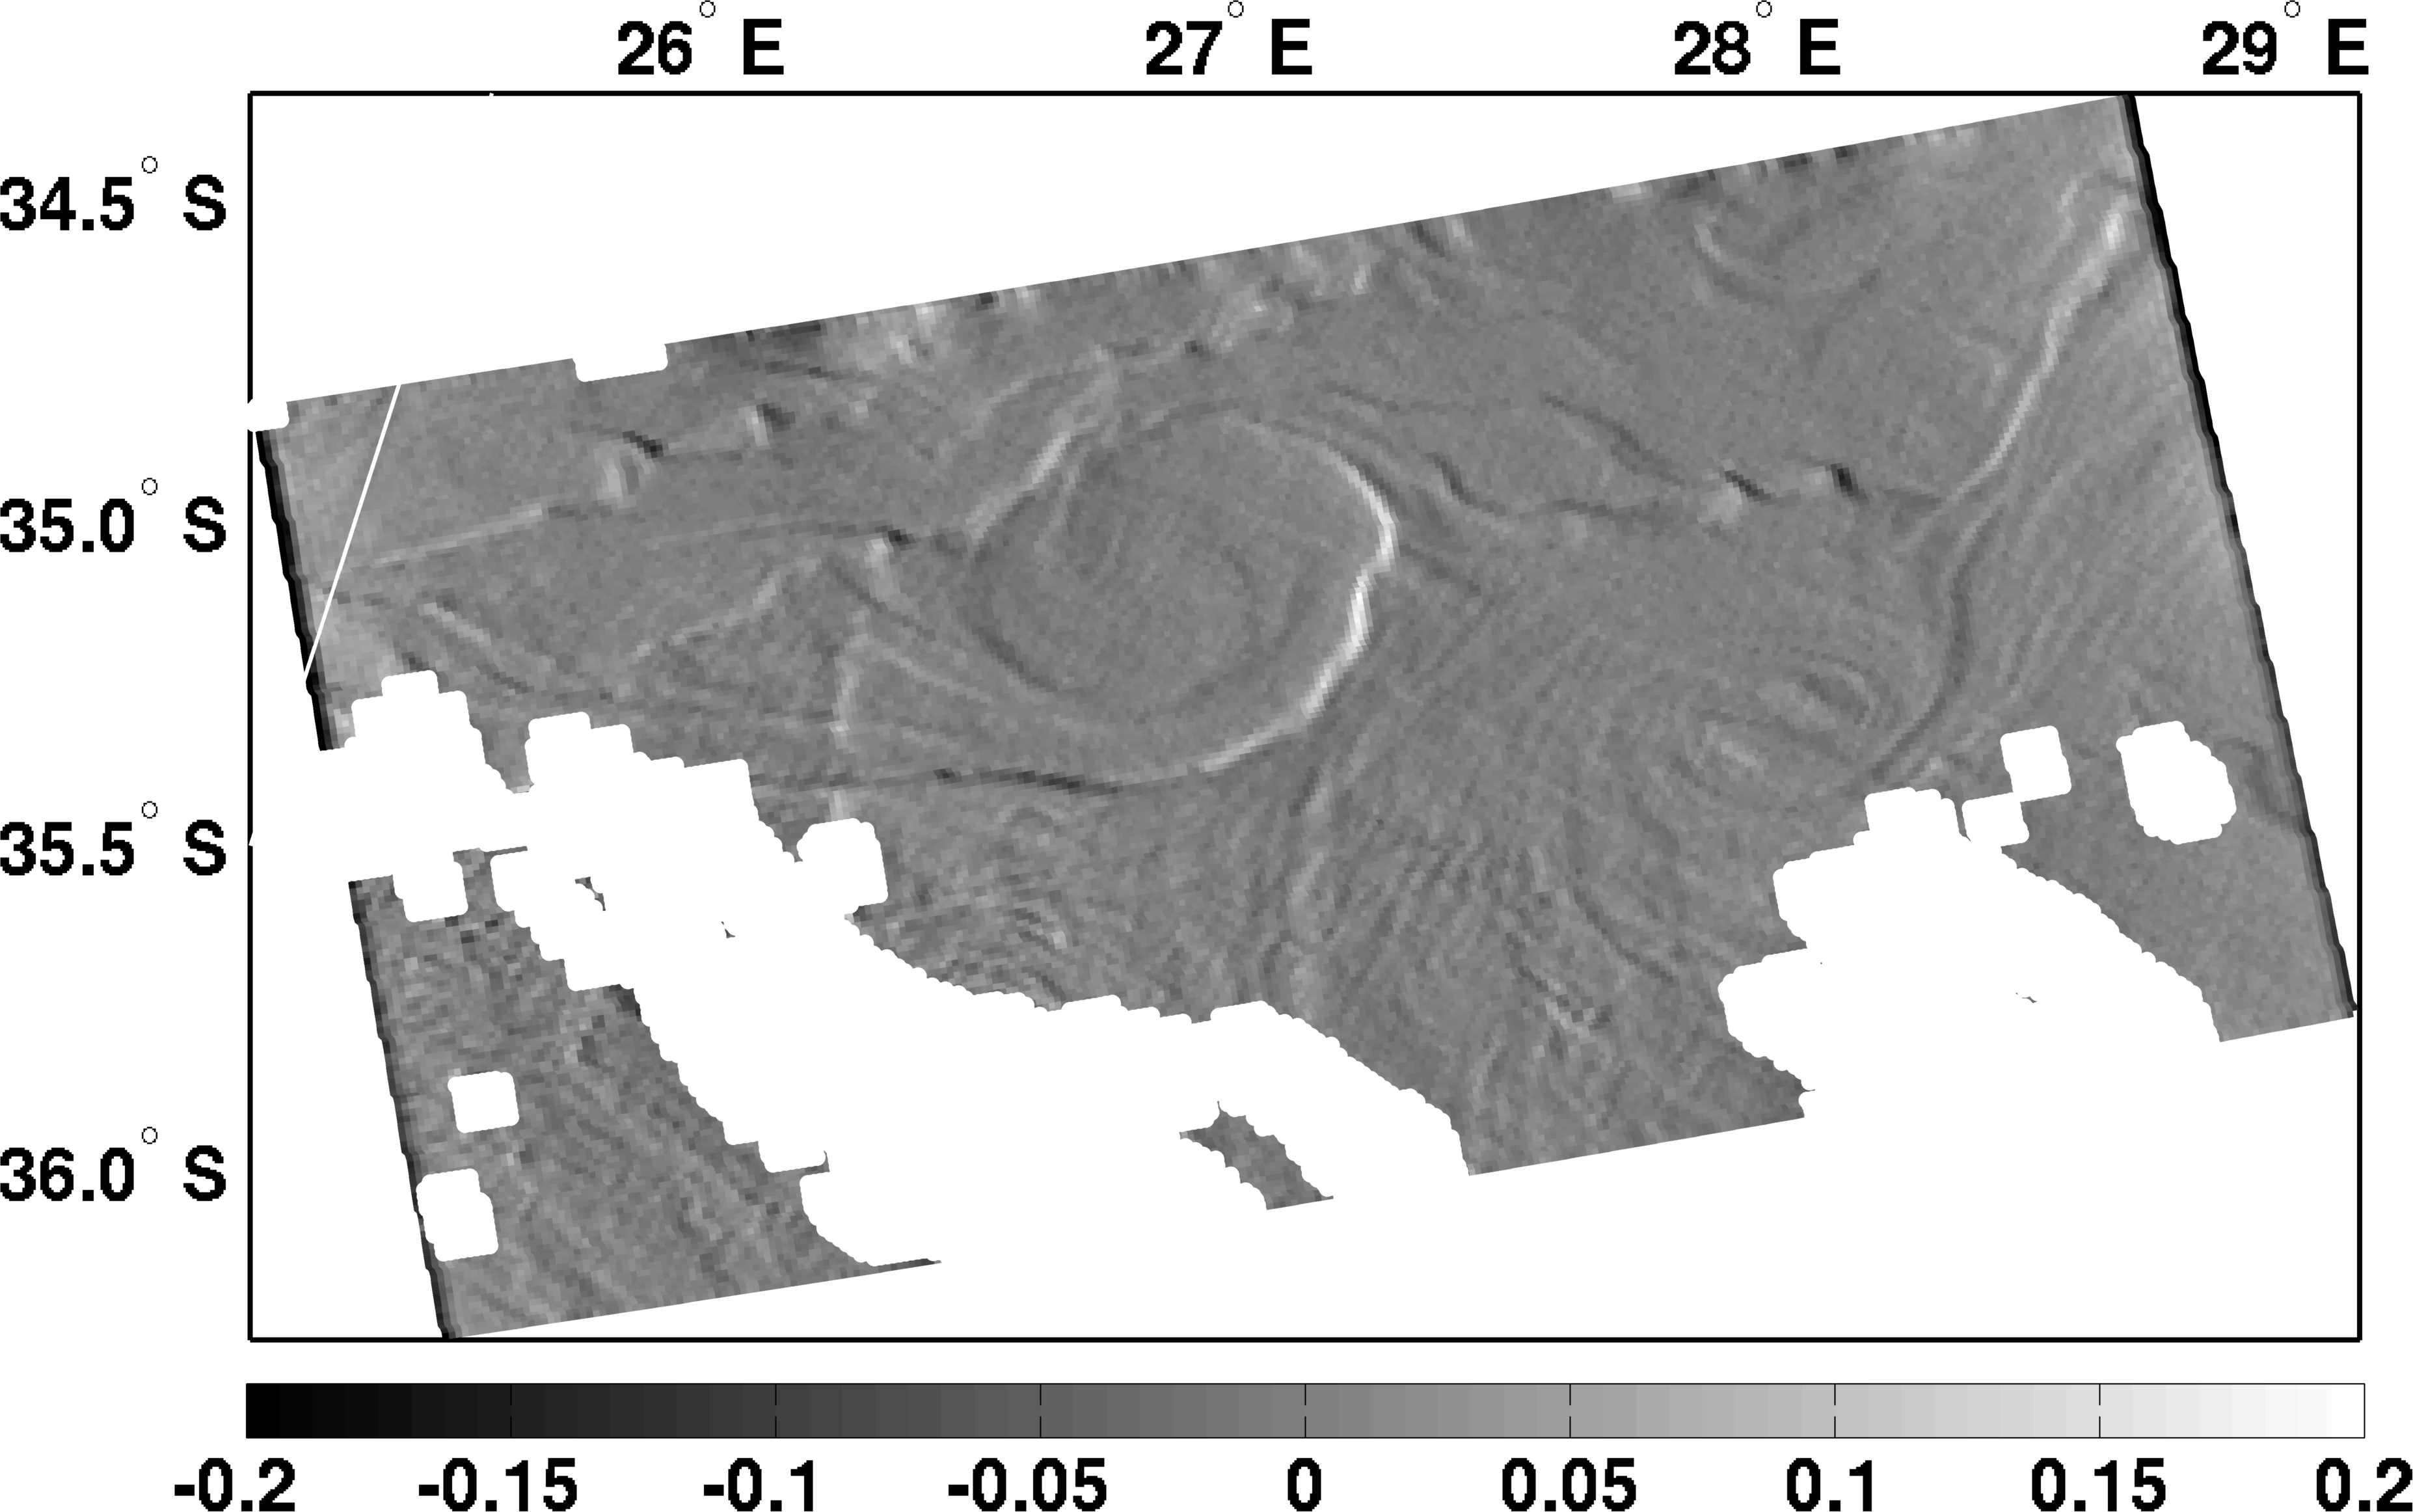
\includegraphics[width=1\linewidth]{fig3_11d}}
	\end{minipage}
    \\
    \floattitle{(а) Дивергенция поля поверхностного течения, полученное по полю ТПО (Рисунок~3\ref{fig:3.9a}). Яркие области на рисунке (а) соответствуют конвергенции течения, а тёмные -- дивергенции (детальнее см. подпись к Рисунку~\ref{fig:3.6b}). Другие рисунки -- симуляции RIM модели поверхностных проявлений грибовидной структуры, представленной в виде контрастов СКН (б), обрушения волн (в), и контрастов УЭПР (г)}
    \caption{Фрагменты восстановленного по ТПО поля дивергенции поверхностного течения и смоделированных характеристик: контрастов СКН, обрушений волн, и контрастов УЭПР}
    \label{fig:3.11}
\end{figure}


Сравнив результаты моделирования RIM, приведённые на Рисунке~\ref{fig:3.11}, с упрощёнными выражениями в уравнениях \eqref{eq:1.5}, \eqref{eq:1.7}, \eqref{eq:1.8} и \eqref{eq:1.9}, у нас появляется возможность найти константу пропорциональности для дальнейшего использования упрощённых решений в практических целях. Мы пришли к следующим соотношениям:



\begin{equation} \label{eq:3.11)} \begin{array}{l} {\frac{\tilde{s}^{2} }{s^{2} } =-\frac{c_{s} }{u_{*}^{} (k_{c} K)^{1/2} } \nabla \cdot {\it u}} \\ {\frac{\tilde{q}_{} }{q_{0} } =-c_{q} \ln \left(\frac{u_{*} k_{b} }{g^{1/2} K^{1/2} } \right)\frac{g}{u_{*}^{2} k_{b} } \omega _{b}^{-1} \nabla \cdot {\it u}} \end{array} \end{equation} 



\noindent где $c_{s} =$ 180 и $c_{q} =$ 470 при $k_{c} =(g/\gamma )^{1/2} $ и $k_{b} =k_{R} /10$ ($\gamma $ - поверхностное натяжение, $k_{R} $ - волновое число радара).

В конечном счёте, анализ РСА и СКН сигнатур суб- и мезомасштабной динамики верхнего слоя Океана отражает отчётливое текстурное сходство с полями конвергенции/дивергенции, хотя незначительные различия в контрастах паттернов всё же наблюдаются. Предположительно, причиной этому могут служить:

\begin{enumerate}
\item  несовершенное восстановление поверхностного течения и поля дивергенции по данным ТПО MODIS;

\item  неточности в поле локального ветра, ветровом дрейфе, Экмановском течении и оценках инерциальных течений;

\item  пространственно-временная эволюция мезомасштабных особенностей за пятичасовой интервал между съёмками ASAR и MODIS.
\end{enumerate}

Тем не менее, общее соответствие очень обнадёживает и прекрасно демонстрирует возможности для получения количественных оценок динамики верхнего слоя Океана по мультисемнсорным поверхностным проявлениям мезомасштабных особенностей.



\newpage


\section{Выводы по главе} \label{sec:3.4}


На примере внутренних волн (ВВ) продемонстрировано, что блик является отличным ``инструментом'' для исследования динамики Океана. Известно что ВВ являются простейшим типом течений и идеальным объектом для тестирования любого метода. Так, в работе \citep{1986} показано, что усиление обрушений волн (в несколько раз по отношению к фоновым значениям) возникало при заглублении термоклина, и почти исчезало при поднятии термоклина, т.е. усиление/подавление обрушений ветровых волн происходило в зонах конвергенции/дивергенции течений индуцированных ВВ на морской поверхности.

В данной главе показано, что поверхностные проявления ВВ также хорошо видны и в модуляциях уклонов морской поверхности. Это связано с усилением среднеквадратичного (СКН) в зонах конвергенции течения ВВ, в то время как подавление наблюдается в зонах дивергенции. Эта связь между аномалиями СКН и дивергенцией поверхностного течения ВВ идентична модуляциям обрушений ветровых волн, вызванных ВВ, наблюдаемых Дуловым и др. в 1986 \citep{1986} в этом же районе исследования.

В отличии от ВВ, вопрос о возможности идентификации мезомасштабных течений остается открытым. До сих пор численное понимание механизмов формирования РСА изображений шероховатости морской поверхности под воздействием полей дивергенции и конвергенции поверхностного течения было недостаточным.  В данной работе предлагается и применяется новый синергетический подход, основанный на совместном использовании оптических, включая инфракрасные каналы, и радиолокационных изображений для исследования поверхностных проявлений процессов в Океане.

Предложен и применён новый синергетический подход для анализа данных РСА и оптических спектрометров, включая инфракрасные каналы. В рамках предложенного подхода используются исходные комбинации полей ТПО, полученных по инфракрасным оптическим данным, данные о шероховатости морской поверхности, -- по изображениям солнечного блика и РСА. На основании полученных полей делается вывод о реализуемости спутниковой диагностики Океана.

Очевидно, что применённый синергетический подход ясно демонстрирует прекрасное соответствие аномалий СКН, реконструированных по изображению солнечного блика (сформированных полным спектром волн, от капиллярных до энергонесущих), с аномалиями шероховатости, восстановленных по РСА изображению. Далее обнаружено, что оба поля находятся в пространственном соответствии с фронтальными областями, представляющими градиенты ТПО. Поскольку типичная фронтальная область состоит из вдоль-фронтальной струи течения с интенсивной перекрестно-фронтальной динамикой и вертикальными движениями, мы ожидали получить именно эти результаты, на основании \citep{Kudryavtsev2005,Johannessen2005}.

Основываясь на предположении, что циркуляция верхнего слоя Океана квази двумерно, поле поверхностного квазигеострофического течения (КГТ) восстанавливается по снимку данных ТПО, следуя теории поверхностной квазигеострофической (ПКГ) динамики. 

Поскольку результирующее поле КГТ является бездивергентным, его прямое взаимодействие с ветровыми волнами приводит к слабому проявлению на поверхности особенностей мезомасштабного течения, как уже было показано в \citep{Kudryavtsev2005,Johannessen2005}. Поэтому, скорее всего, механизм проявления несколько другой. 

Взаимодействие вызванных ветром в верхнем слое потоков с полем КГТ (путём Экмановского адвективного механизма, и диабатического механизма перемешивания, как предложено в \citep{Klein1990,Garrett1981}  приводит к генерации достаточно сильного агеострофического течения, которое, в свою очередь, приводит к большим конвергенционным и дивергенционным поверхностным потокам, проявления которых мы и наблюдаем. В соответствии с предлагаемым предположением, интенсивная перекрестно-фронтальная динамика возникает как близ резких горизонтальных градиентов поля завихренности КГТ, так и в районе сильных вертикальных градиентов поля скорости КГТ.

В соответствии с вышеизложенным, можно рассматривать наблюдаемое поразительное соответствие между аномалиями шероховатости и градиентами ТПО в качестве ``экспериментального подтверждения'' того факта, что влияние дивергенции поверхностного течения на короткие ветровые волны есть основной механизм, приводящий к поверхностным проявлениям мезомасштабных особенностей течения в виде аномалий ``шероховатости'' морской поверхности. 

Помимо этого, стоит отметить, что корреляция между аномалиями шероховатости морской поверхности и модельной дивергенцией поверхностного течения наводит на мысль о надёжности модельного фреймворка для восстановления мезомасштабных поверхностных течений.

Поле поверхностного течения, восстановленное по данным ТПО MODIS и ветру ASAR, также использовались в качестве входных параметров модели формирования РЛ-изображения RIM, для симулирования РСА УЭПР и СКН сигнатур. Реконструированное поле чётко отражает, что наблюдаемые аномалии на изображении РСА, вместе с аномалиями поля СКН, восстановленного по данным MODIS, представляют поверхностные проявления зон конвергенции и дивергенции океанического течения вдоль меандрирующих фронтов и вихрей.

В результате реализации подхода восстанавливаются следующие поля:

\begin{itemize}
	\itemsep0em
	\item Квазигеострофического течения
	\item поля РСА-ветра
	\item полные поля течений -- квазигеострофика + ветровой дрейф + агеострофическая циркуляция
	\item поля дивергенции течений
	\item поля шероховатости (в частности СКН)
\end{itemize}

Подытоживая, можно утверждать, что предложенный синергетический подход, объединяющий ТПО, яркость солнечного блика и данные РСА, дополненный и другими источниками данных более низкого разрешения (например, альтиметров и скаттерометров), предоставляет согласующееся численное решение положения и интенсивности зон конвергенции/дивергенции (апвеллинга/даунвеллинга) поверхностного течения. А это, в свою очередь, важный и многообещающий шаг в сторону прогресса численной интерпретации и понимания динамики верхнего слоя Океана по двумерным изображениям его поверхностных проявлений.

\clearpage